\documentclass{sig-alternate}

%\usepackage[numbers, sort, compress]{natbib}
\usepackage{graphicx}
\usepackage{amsmath}
\usepackage{amssymb}
\usepackage{color}
\usepackage{ifpdf}
%\usepackage{mdwlist}

%\usepackage{dcolumn}
\usepackage{float}
\usepackage[utf8]{inputenc}
\usepackage{multirow}
\usepackage{rotating}
\usepackage{subfigure}



%\usepackage[numbers, sort, compress]{natbib}
%\usepackage{latex8}
%\usepackage{float}
%\usepackage{times}    
\usepackage{url}
\usepackage{booktabs}
\usepackage{listings}   
\usepackage{paralist}    
\usepackage{wrapfig}    
%\usepackage[footnotesize,it]{caption}
\usepackage{multirow}
\usepackage{ifpdf}
%\usepackage{srcltx}
%\usepackage{subfigure}
\usepackage{xspace}
\usepackage{keyval}  
\usepackage{color}
\usepackage{comment}

\definecolor{listinggray}{gray}{0.95}
\definecolor{darkgray}{gray}{0.7}
\definecolor{commentgreen}{rgb}{0, 0.4, 0}
\definecolor{darkblue}{rgb}{0, 0, 0.4}
\definecolor{middleblue}{rgb}{0, 0, 0.7}
\definecolor{darkred}{rgb}{0.4, 0, 0}
\definecolor{brown}{rgb}{0.5, 0.5, 0}

\usepackage[normalem]{ulem}
\makeatletter
\def\cyanuwave{\bgroup \markoverwith{\lower3.5\p@\hbox{\sixly \textcolor{cyan}{\char58}}}\ULon}
\def\reduwave{\bgroup \markoverwith{\lower3.5\p@\hbox{\sixly \textcolor{red}{\char58}}}\ULon}
\def\blueuwave{\bgroup \markoverwith{\lower3.5\p@\hbox{\sixly \textcolor{blue}{\char58}}}\ULon}
\font\sixly=lasy6 % does not re-load if already loaded, so no memory problem.
\makeatother

\newif\ifdraft
\drafttrue
\ifdraft
\usepackage{xcolor}
\newcommand{\onote}[1]{ {\textcolor{cyan} { (***Ole: #1) }}}
\newcommand{\terminology}[1]{ {\textcolor{red} {(Terminology used: \textbf{#1}) }}}
\newcommand{\owave}[1]{ {\cyanuwave{#1}}}
\newcommand{\jwave}[1]{ {\reduwave{#1}}}
\newcommand{\alwave}[1]{ {\blueuwave{#1}}}
\newcommand{\jhanote}[1]{ {\textcolor{red} { ***shantenu: #1 }}}
\newcommand{\alnote}[1]{ {\textcolor{green} { ***andreL: #1 }}}
\newcommand{\amnote}[1]{ {\textcolor{blue} { ***andreM: #1 }}}
\newcommand{\smnote}[1]{ {\textcolor{brown} { ***sharath: #1 }}}
\newcommand{\pmnote}[1]{ {\textcolor{brown} { ***Pradeep: #1 }}}
\newcommand{\msnote}[1]{ {\textcolor{cyan} { ***mark: #1 }}}
\newcommand{\mrnote}[1]{ {\textcolor{purple} { ***melissa: #1 }}}
\definecolor{orange}{rgb}{1,.5,0}
\newcommand{\aznote}[1]{ {\textcolor{orange} { ***ashley: #1 }}}
\definecolor{dandelion}{cmyk}{0,0.29,0.84,0}
\newcommand{\mtnote}[1]{ {\textcolor{dandelion} { ***matteo: #1 }}}
\newcommand{\note}[1]{ {\textcolor{magenta} { ***Note: #1 }}}
\else
\newcommand{\onote}[1]{}
\newcommand{\terminology}[1]{}
\newcommand{\owave}[1]{#1}
\newcommand{\jwave}[1]{#1}
\newcommand{\alnote}[1]{}
\newcommand{\amnote}[1]{}
\newcommand{\aznote}[1]{}
\newcommand{\athotanote}[1]{}
\newcommand{\smnote}[1]{}
\newcommand{\pmnote}[1]{}
\newcommand{\jhanote}[1]{}
\newcommand{\msnote}[1]{}
\newcommand{\mtnote}[1]{}
\newcommand{\note}[1]{}
\newcommand{\mrnote}[1]{}
\fi

\newcommand{\cloud}{cloud\xspace}
\newcommand{\clouds}{clouds\xspace}
\newcommand{\pilot}{Pilot\xspace}
\newcommand{\pilots}{Pilots\xspace}
\newcommand{\pilotjob}{Pilot-Job\xspace}
\newcommand{\pilotjobs}{Pilot-Jobs\xspace}
\newcommand{\pilotcompute}{Pilot-Compute\xspace}
\newcommand{\pilotcomputes}{Pilot-Computes\xspace}
\newcommand{\pilotdata}{Pilot-Data\xspace}
\newcommand{\pilotdataservice}{Pilot-Data Service\xspace}
\newcommand{\pilotcomputeservice}{Pilot-Compute Service\xspace}
\newcommand{\computedataservice}{Compute-Data Service\xspace}
\newcommand{\pilotmapreduce}{PilotMapReduce\xspace}
\newcommand{\mrmg}{MR-Manager\xspace}
\newcommand{\pstar}{P*\xspace}
\newcommand{\pd}{PD\xspace}
\newcommand{\pj}{PJ\xspace}
\newcommand{\pjs}{PJs\xspace}
\newcommand{\pds}{Pilot Data Service\xspace}
\newcommand{\computeunit}{Compute-Unit\xspace}
\newcommand{\computeunits}{Compute-Units\xspace}
\newcommand{\dataunit}{Data-Unit\xspace}
\newcommand{\dataunits}{Data-Units\xspace}
\newcommand{\du}{DU\xspace}
\newcommand{\dus}{DUs\xspace}
\newcommand{\cu}{CU\xspace}
\newcommand{\cus}{CUs\xspace}
\newcommand{\su}{SU\xspace}
\newcommand{\sus}{SUs\xspace}
\newcommand{\schedulableunit}{Schedulable Unit\xspace}
\newcommand{\schedulableunits}{Schedulable Units\xspace}
\newcommand{\cc}{c\&c\xspace}
\newcommand{\CC}{C\&C\xspace}
\newcommand{\up}{\vspace*{-1em}}
\newcommand{\upp}{\vspace*{-0.5em}}
\newcommand{\numrep}{8 }
\newcommand{\samplenum}{4 }
\newcommand{\tmax}{$T_{max}$ }
\newcommand{\tc}{$T_{C}$ }
\newcommand{\tcnsp}{$T_{C}$}
\newcommand{\bj}{BigJob\xspace}
\newcommand{\MW}{Master-Worker\xspace}
\newcommand{\panda}{PanDA\xspace}
\newcommand{\apples}{AppLeS\xspace}

\newcommand{\I}[1]{\textit{#1}\xspace}
\newcommand{\B}[1]{\textbf{#1}\xspace}
\newcommand{\T}[1]{\texttt{#1}\xspace}
\newcommand{\C}[1]{\textsc{#1}\xspace}

\lstdefinestyle{myListing}{
  frame=single,   
  backgroundcolor=\color{listinggray},  
  %float=t,
  language=C,       
  basicstyle=\ttfamily \footnotesize,
  breakautoindent=true,
  breaklines=true
  tabsize=2,
  captionpos=b,  
  aboveskip=0em,
  belowskip=-2em,
  %numbers=left, 
  %numberstyle=\tiny
}      

\lstdefinestyle{myPythonListing}{
  frame=single,   
  backgroundcolor=\color{listinggray},  
  %float=t,
  language=Python,       
  basicstyle=\ttfamily \footnotesize,
  breakautoindent=true,
  breaklines=true
  tabsize=2,
  captionpos=b,  
  %numbers=left, 
  %numberstyle=\tiny
}



%  \setlength{\parskip}{0.05ex} % 1ex plus 0.5ex minus 0.2ex}
%  \setlength{\parsep}{0pt}
%  %\setlength{\headsep}{0pt}
%  \setlength{\topskip}{0pt}
%  \setlength{\topmargin}{0pt}
%  %\setlength{\topsep}{0pt}
%  \setlength{\partopsep}{0pt}

% This is now the recommended way for checking for PDFLaTeX:


\ifpdf
\DeclareGraphicsExtensions{.pdf, .jpg, .tif}
\else
\DeclareGraphicsExtensions{.eps, .jpg, .ps}
\fi

\tolerance=1000
\hyphenpenalty=10


\usepackage{listings}
\usepackage{paralist}
\usepackage{multirow}
\usepackage{flushend}
\usepackage{lscape}

\lstnewenvironment{code}[1][]%
{
  \noindent
  %\minipage{0.98 \linewidth}
  \minipage{1.0 \linewidth}
    \vspace{0.5\baselineskip}
    \lstset{
        language=Python,
    %    numbers=left,
    %    numbersep=4pt,
        frame=single,
        captionpos=b,
        stringstyle=\ttfamily,
        basicstyle=\scriptsize\ttfamily,
        showstringspaces=false,#1}
}
{\endminipage}


\usepackage{draftwatermark}
%\usepackage[firstpage]{draftwatermark}
\SetWatermarkLightness{0.8}
\SetWatermarkText{Draft}
\SetWatermarkVerCenter{13cm}
\SetWatermarkHorCenter{10cm}
\SetWatermarkScale{1}


\begin{document}
% \conferenceinfo{HPDC'13}{2013, New York, USA}
% \conferenceinfo{ECMLS'11,} {June 8, 2011, San Jose, California, USA.}
\CopyrightYear{2015}
% \crdata{978-1-4503-0702-4/11/06}
% \clubpenalty=10000
% \widowpenalty = 10000

\title{A Comprehensive Perspective on the Pilot-Abstraction}

%\jhanote{either abstraction is singular and therefore ``the'', or we use the
%plural form}}

\numberofauthors{3}

\author{
  \alignauthor
  Matteo Turilli \\
    \affaddr{RADICAL Laboratory, ECE}\\
    \affaddr{Rutgers University}\\
    % \email{}
  % 2nd. author
  \alignauthor
  Mark Santcroos\\
    \affaddr{RADICAL Laboratory, ECE}\\
    \affaddr{Rutgers University}\\
    % \email{}
  % 3rd. author
  \alignauthor
  Shantenu Jha\titlenote{Corresponding author}\\
    \affaddr{RADICAL Laboratory, ECE}\\
    \affaddr{Rutgers University}\\
    % \email{}
  % use '\and' if you need 'another row' of author names
  % \and
  % % 4th. author
  % \alignauthor Lawrence P. Leipuner\\
  %   \affaddr{Brookhaven Laboratories}\\
  %   \affaddr{Brookhaven National Lab}\\
  %   \affaddr{P.O. Box 5000}\\
  %   \email{lleipuner@researchlabs.org}
  % % 5th. author
  % \alignauthor Sean Fogarty\\
  %   \affaddr{NASA Ames Research Center}\\
  %   \affaddr{Moffett Field}\\
  %   \affaddr{California 94035}\\
  %   \email{fogartys@amesres.org}
  % % 6th. author
  % \alignauthor Charles Palmer\\
  %   \affaddr{Palmer Research Laboratories}\\
  %   \affaddr{8600 Datapoint Drive}\\
  %   \affaddr{San Antonio, Texas 78229}\\
  %   \email{cpalmer@prl.com}
}

\date{}
\maketitle

\begin{abstract}

  This paper provides a comprehensive analysis of the evolution, functional
  properties and implementations of the pilot abstraction, the most common
  incarnation of which are the many \pilotjob software systems that have been
  gaining rapid adoption among various scientific communities. For example,
  \pilotjobs systems are used to provide more than 700 million CPU hours a year
  to the Open Science Grid (OSG) communities and to process up to 5 million jobs
  a week for the ATLAS experiment. Notwithstanding the growing impact of
  \pilotjobs on scientific research, there is no agreement upon their
  definition, no clear understanding of the underlying abstraction and paradigm,
  no shared best practices or interoperability among their implementations. This
  lack of foundational understanding and of design convergence is hindering the
  full exploitation of the \pilotjobs potential dispersing the available
  resources across a fragmented development landscape.  This paper offers the
  conceptual tools to promote shared understanding of the \pilot paradigm while
  critically reviewing the state of the art of \pilotjobs implementations. Five
  main contributions are provided: (i) an analysis of the motivations and
  evolution of the \pilotjob abstraction; (ii) an outline of the minimal set of
  distinguishing functionalities; (iii) the definition of a core vocabulary to
  reason consistently about \pilotjobs; (iv) the description of core and
  auxiliary properties of \pilotjobs systems; and (v) a critical review of the
  current state of the art of their implementations. These contributions are
  brought together to illustrate the defining characteristics of the \pilotjob
  paradigm, its generality, and the main opportunities and challenges posed by
  its support of distributed computing.

  % There is no agreed upon definition of \pilotjobs; however a functional
  % attribute of \pilotjobs that is generally agreed upon is they are
  % tools/services that support multi-level and/or application-level scheduling
  % by providing a scheduling overlay on top of the system-provided schedulers.
  % Nearly everything else is either specific to an implementation, open to
  % interpretation or not agreed upon. For example, are \pilotjobs part of the
  % application space, or part of the services provided by an infrastructure? We
  % will see that close-formed answers to questions such as whether \pilotjobs
  % are system-level or application-level capabilities are likely to be elusive.
  % Hence, this paper does not make an attempt to provide close-formed answers,
  % but aims to provide appropriate context, insight and analysis of a large
  % number of \pilotjobs, and thereby bring about a hitherto missing consistence
  % in the community's appreciation of \pilotjobs.  Specifically this paper aims
  % to provide a comprehensive perspective of \pilotjobs. A primary motivation
  % for this work stems from our experience when looking for an interoperable,
  % extensible and general-purpose \pilotjob; in the process, we realized that
  % such a capability did not exist. The situation was however even more
  % unsatisfactory: in fact there was no agreed upon definition or conceptual
  % framework of \pilotjobs.  To substantiate these points of view, we begin by
  % discussing some existing \pilotjobs and the different aspects of these
  % \pilotjobs, such as the applications scenarios that they have been used and
  % how they have been used. The limited but sufficient sampling highlights the
  % variation, and also provides both a motivation and the basis for developing
  % an implementation agnostic terminology and vocabulary to understand
  % \pilotjobs; Section \S3 attempts to survey the landscape/eco-system of
  % \pilotjobs.  With an agreed common framework/vocabulary to discuss and
  % describe \pilotjobs, we proceed to analyze the most commonly utilized
  % \pilotjobs and in the process provide a comprehensive survey of \pilotjobs,
  % insight into their implementations, the infrastructure that they work on,
  % the applications and application execution modes they support, and a frank
  % assessment of their strengths and limitations.  An inconvenient but
  % important question -- both technically and from a sustainability perspective
  % that must be asked: why are there so many similar seeming, but partial and
  % slightly differing implementations of \pilotjobs, yet with very limited
  % interoperability amongst them?  Examining the reasons for this
  % state-of-affairs provides a simple yet illustrative case-study to understand
  % the state of the art and science of tools, services and middleware
  % development.  Beyond the motivation to understand the current landscape of
  % \pilotjobs from both a technical and a historical perspective, we believe a
  % survey of \pilotjobs is a useful and timely undertaking as it provides
  % interesting insight into understanding issues of software sustainability.
  %
  % believe that a survey of \pilotjobs provides and appreciation for
  % the richness of the \pilotjobs landscape.  is
  % not to discuss the \pstar conceptual framework, but That led to
  % the \pstar model.
\end{abstract}

\section{Introduction}
\label{sec:intro}

% \jhanote{Building tools and components that have well-defined and
%   well-characterized behavior, including performance. This leads to descriptive
%   models of pilot-jobs, which while pervasive in distributed computing, are
%   conspicuous by their absence in high-performance and data-intensive computing.
%   By providing a firm theoretical underpinning  pilot-jobs [3], one can
%   provide a more “programmable” and flexible yet common pilot-job for different
%   types of distributed infrastructure, and also extend the concept of pilot-jobs
%   to high-performance and data-intensive computing [4]}

The seamless uptake of distributed computing infrastructures by scientific
applications has been limited by the lack of pervasive and simple-to-use
abstractions at the development, deployment, and execution level. \pilotjob is
arguably one of the most widely-used distributed computing abstractions, as
suggested by the proliferation of \pilotjob systems used in production
cyberinfrastructure.

A variety of \pilotjob systems have emerged: Condor-G/ Glide-in~\cite{condor-g},
Swift~\cite{Wilde2011}, DIANE~\cite{Moscicki:908910},
DIRAC~\cite{1742-6596-219-6-062049}, \panda~\cite{1742-6596-219-6-062041},
ToPoS~\cite{topos}, Nimrod/G~\cite{10.1109/HPC.2000.846563},
Falkon~\cite{1362680} and
MyCluster~\cite{1652061,mycluster-clade,mycluster-cluster} to name a few. These
systems are for the most part functionally equivalent as they support the
decoupling of workload submission from resource assignment. Nonetheless, their
implementations often serve specific use cases, target specific resources, and
lack in interoperability.

% The situation is reminiscent of the proliferation of functionally similar yet
% incompatible workflow systems, where in spite of significant {\it a
% posteriori} effort on workflow system extensibility and interoperability,
% these objectives remain difficult if not unfeasible.

% \pilotjobs excel in terms of the number and types of applications that use
% them, as well as the number of production distributed cyberinfrastructures
% that support them. \msnote{ref?}

% \mtnote{Should we use just `pilot'}\jhanote{I think you have proposed a
% graceful transition: from pilotjobs to pilotsystems? If so, should we stick
% with pilotjobs here?}

The fundamental reason for the proliferation of \pilotjob systems is that they
provide a simple solution to the rigid and static resource management
historically found in high-performance and distributed computing (HPDC).  There
are two ways in which \pilotjobs break free of the rigid resource utilization
model: (i) through a process often referred to as
late-binding~\cite{moscicki2011,glatard2010,delgado2014}, \pilotjobs make the
selection of heterogeneous and dynamic resources easier and effective; and (ii)
\pilotjobs decouple the workload specification from the task management.  The
former results in the ability to utilize resources ``dynamically'', the latter
simplifies the placement of workloads on those resources.

% management of improving the efficiency of task assignment while shielding
% applications from having to manage tasks across such resources.

%   \onote{I think the most important reasons why Pilot Jobs being so
%     popular (and re-invented over and over again) is that they allow
%     the execution of small (i.e., singe / few-core) tasks efficiently
%     on HPC infrastrucutre by massively reducing queueing time. HPC
%     sites (from schedulers to policies) have always been (and still
%     are) discrimatory against this type of workload in favor of the
%     large, tightly-coupled ones. Pilot-Jobs try to counteract. While
%     this is certainly not the main story that we want to tell, this
%     should IMHO still be mentioned. } \jhanote{This is definitely one
%     of the main reasons, but as Melissa pointed out it during RADICAL
%     call, it is by no means the only reason. Need to get the different
%     reasons down here.. then find a nice balance and description}

 %(thus providing {\it post-facto} justification of its needs)

% \mtnote{Should we have a paragraph explaining the core contribution offered by
% this paper?} \jhanote{yes} \mtnote{Should I write a first draft of it?}

Though mostly as a pragmatic solution to the need of improving throughput
performance of distributed applications, \pilotjobs have been almost exclusively
developed within preexisting systems and middleware dedicated to specific
scientific requirements. As a consequence, the development of \pilotjobs have
not been grounded on a robust understanding of underpinning abstractions, or on
a well-understood set of dedicated design principles. The functionalities and
properties of \pilotjobs have been understood mostly in relation to the needs of
the containing software systems or of the user cases justifying their
development.

This approach is not problematic in itself and has led to effective
implementations that serve many million jobs a year on diverse computing
platforms~\cite{maeno2014,katz2012}. However, the lack of an explicit
appreciation of the computing paradigm underlying \pilotjobs has undermined the
full development of dedicated designs and implementations. This limitation is
well illustrated not only by the effort duplication but also by an overall
immaturity of the available systems in terms of functionalities, flexibility,
portability, interoperability, and, most often, robustness.

This survey is motivated by the fact that, in spite of the demonstrated
potential and proliferation of \pilotjob systems, there remains significant lack
of clarity and understanding about the \pilotjob abstraction. We believe this
results in unfulfilled and lost potential as well as significant overhead and
repetition of effort.

This paper offers a critical analysis of the current state of the art providing
the conceptual tooling required to appreciate the properties of the \pilot
paradigm, i.e. the abstraction and the methodology underlying \pilotjobs
systems. The remainder of this paper is divided into four sections.
\S\ref{sec:history} offers a critical review of the functional underpinnings of
the \pilot abstraction and how it has been evolving into \pilotjob systems and
systems with pilot-like characteristics.

In~\S\ref{sec:understanding}, the minimal set of capabilities and properties
characterizing the design of a \pilotjob system are derived. A vocabulary is
then defined to be consistently used across different designs and
\pilotjob system implementations.

In~\S\ref{sec:analysis}, the focus shifts from analyzing the design of a
\pilotjob system to critically reviewing the characteristics of a representative
set of its implementations. Core and auxiliary implementation properties are
introduced and then used alongside the functionalities and terminology defined
in~\S\ref{sec:understanding} to compare \pilotjob systems implementations.

Finally,~\S\ref{sec:discussion} closes the paper by outlining the \pilot
paradigm, arguing for its generality, and elaborating on how it impacts and
relates to both other middleware and the application layer. The outcome of the
critical review of the current implementation state of the art is used to give
insights about the future directions and challenges faced by the \pilot
paradigm.

\jhanote{these last two are not reasons for the success of pilot-jobs. they
  arise as a consequence of the success} The \pilotjob abstraction is also a
promising route to address specific requirements of distributed scientific
applications, such as coupled-execution and application-level
scheduling~\cite{ko-efficient,DBLP:conf/hpdc/KimHMAJ10}. Another concern often
addressed by \pilotjobs is fault tolerance which commonly refers to the ability
of the \pilotjob system to verify the execution environment before executing
jobs.

\mtnote{We need to verify if all this is described in 4.2. For example, what
  \pilot systems offer fault-tolerance? Runs on heterogeneous resources?
  Dynamic?} \jhanote{I'll be rewriting the Introduction, so please consider
  introduction locked.}


% -----------------------------------------------------------------------------
% SECTION 2
%
%\section{Functional Underpinnings and Evolution of Pilot Abstraction}
\section{Evolution of Pilot Abstraction and Systems}
\label{sec:history}

% -----------------------------------------------------------------------------
% Version 0.1
% -----------------------------------------------------------------------------

% \subsection{A Functional Approach to Pilot-Jobs}
% Many scientific communities began running into the same issues:

% As distributed systems grew in capacity and capability, they also grew
% in complexity and heterogeneity. For example, many machines
% implemented their own batch queuing systems, and oftentimes these
% systems varied from machine to machine.\msnote{The part after the
% comma is kind of implicit by the part before} The wide use of
% heterogenous resources, resulted in the need for workload management
% across these resources.  In order to harness the power of these
% heterogeneous resources to run jobs, one particular solution proposed
% is that of
% \pilotjobs

% , which have historically been used as a means of solving these
% issues. This gave rise to the the need for job submission management
% via batch queuing systems and middleware access also grew. We briefly
% discuss some specific uses of \pilotjobs below.

% \pilotjobs are most commonly used for the execution of many tasks
% through the use of a container job. They are often measured by their
% throughput, that is, the number of tasks that they can complete per
% second (tps)\msnote{I dont think we use tps further in the paper}, or
% alternatively, by the total number of tasks executed. As such,
% \pilotjobs are used to achieve high-throughput, for example, when
% using genome sequencing techniques \msnote{Arguably genome
% applications are not the most illustrative example of high throughput
% tasks getting benefit out of pilot-jobs} or ensemble-based
% applications. \pilotjobs have also been used for parameter sweeps,
% chained tasks, and loosely-coupled but distinct tasks. %note to self:
% cite these with papers

% Multi-scale simulations have also benefited from the use of
% \pilotjobs. A framework for load balancing via dynamic resource
% allocation for coupled multi-physics (MPI-based) simulations using
% \pilotjobs was demonstrated in Ref.~\cite{ko-efficient}. This was
% achieved by dynamically assigning more processors to jobs with longer
% runtimes, so that these jobs could accomplish their workload in the
% same amount of wall-clock time as those with shorter runtimes. This
% led to an overall reduction of jobs that were waiting to communicate
% via MPI, and an overall reduction of the total simulation runtime.

% \pilotjobs can be used for  simulations with varying numbers of tasks
%  to complete, for example, molecular dynamics simulations requiring
%  task restart. These types of simulations may start with a fixed
%  number of tasks but spawn more tasks in order to continue simulating.
%  \pilotjobs can be utilized for these types of dynamic simulations,
%  because new tasks can be fed to the \pilot at any time within a given
%  runtime. Without \pilotjobs, these simulations would have to be
%  resubmitted to the batch queue and wait for their time to become
%  active again~\cite{luckow2009adaptive}.

% \pilotjobs have also been used to avoid queue wait times for many jobs
% \msnote{I think we just said this above in the high-throughput case}
% as well as harness and utilize different resources (with different
% batch queueing systems) to do \textit{scale-across} simulations. As a
% fault tolerant mechanism, many \pilotjob systems monitor failed jobs
% and have the ability to restart them within the given time frame of
% the \pilotjob's total
% runtime~\cite{1742-6596-219-6-062049,condor-g,nilsson2011atlas}.

% In order to appreciate \pilotjobs, we outline the evolution of
% \pilot-like capabilities ultimately leading to the creation of the
% first actual \pilotjob. We present a brief chronological order of
% \pilotjob-like systems, beginning with simple Master-Worker-based
% applications through advanced workload management systems.

% \subsubsection*{The Evolution of \pilotjobs}\label{sssec:evolution}

% \pilotjobs provide the ability to distribute workload across multiple
% systems and offer an easy way to schedule many jobs at one time. This
% in turn improves the utilization of resources\msnote{why?}, reduces
% the net wait time of a collection of tasks, and also prevents
% saturation of resource batch queuing systems from high-throughput
% simulations where many jobs need to be run at one time\msnote{I dont
% understand the last claim}. While early \pilot-systems solely provided
% this placeholder job mechanism, many of these system evolved to more
% complex workload management systems. As applications began to utilize
% distributed cyberinfrastructure, the workloads grew from small sets of
% short running jobs to many jobs with either short or potentially long
% runtimes. There was a need for more complex management of these
% workloads and additional capabilities for user-level control of the
% tasks that would be executed within the placeholder job. This drove
% the creation of the modern idea of \pilots \msnote{Kind of an ambigous
% statement, like all statements that include the word "modern" :-)}

% \pilotjob systems differ in their focus and architecture. Our
% preliminary survey of existing \pilotjobs helped to identify three
% major layers that these systems exhibit: (i) core \pilotjob
% functionality - this provides the minimally complete set of
% capabilities for a simple \pilotjob, (ii) advanced \pilotjob
% functionality - a system that offers all of (i) plus a more
% sophisticated resource management mechanism, and (iii) higher-level
% \pilot-based frameworks - frameworks utilize \pilots for a specific
% use case, e.\,g.\ workflows or data analytics.

% \onote{These are not necessarily 'layers'. The more I think about it,
% the whole idea of 'layers' doesn't make so much sense if we want to
% distinguish between core and advanced systems / frameworks. I think
% discussing these 'functionality' along \textbf{orthogonal components}
% (that doesn't necessarily build upon each other) would make more
% sense. My (and ALs) comment w.r.t Figure 1 is related to this.}
% \msnote{I'm tempted to at this stage in the paper use a very high
% level figure to simply support the explanation of the pilotjob
% concept.}

% As one can intuit from the above descriptions, existing \pilotjob
% systems maybe overlap and overflow into these different layers, and
% each layer builds upon the previous one. Therefore, we use these
% classification layers only as a means to explain the basic progression
% of a \pilotjob system from simple scheduling reservation mechanisms to
% more complete job management systems. A more semantically-rich
% terminology and classification scheme will be presented in Sections
% \ref{sec:vocab} and \ref{sec:analysis}.\msnote{I think the whole layering
% discussion can go.}


% Figure~\ref{fig:figures_classification} categorized \pilotjob systems
% into three layers: (i) core \pilotjob systems that solely provide a
% simple \pilot capability, (ii) advanced \pilotjob systems that offer
% sophisticated resource management capabilities based on \pilots, and
% (iii) higher level \pilot-based frameworks that utilize \pilots for a
% specific use case, e.\,g.\ workflows or data analytics. One of the
% important aspects of these layers is that they often overlap or have
% evolved from one another. Therefore, it is hard to classify

% \begin{figure}[t]
%	\centering
%		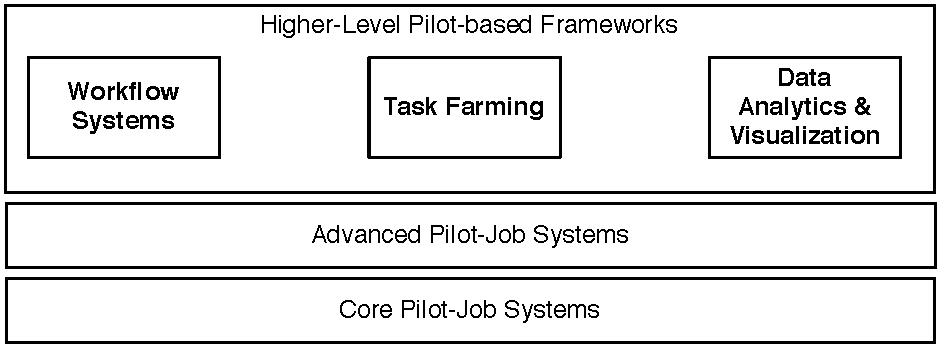
\includegraphics[width=0.45\textwidth]{figures/classification}
%	\caption{Pilot-Job Classification: Different PJ systems focus
%         on different parts of the distributed computing stack: (i)
%          PJ systems that solely provide the \pilot capability, (ii)
%          systems that offer resource management capabilities based on
%          \pilots and (iii) applications, tools and services that
%          utilize \pilots for resource management. \jhanote{we should
%            make the three levels of the diagram consistent with the
%            three categories, ``core PJ'' , ``advanced PJ'' and
%            ``higher-level PJs'' . Also earlier comment about adding
%            ``higher-level pilot-based frameworks'' to ``higher-level
%            frameworks that can use pilot-jobs''.}}  \alnote{mention
%          that these layers are not cleanly separated, add
%          capabilities (outside)/properties (internal) of
%          each layer, what is the overlap between the layers (how they
%          interrelated?, what is the overlap?)?}
%          \onote{IMHO this figure doesn't really help to explain things
%          and is also wrong (see AL's comment above). I think we should
%          get rid of it.  } \msnote{+1}
%	\label{fig:figures_classification}
%\end{figure}

% In this section, we give a brief overview of different \pilotjob
% systems. As grid computing advanced in its size and capabilities, the
% need for job scheduling and time-sharing became more prevalent. Batch
% queuing systems were installed to solve this problem, wherein a login
% node accepted all job submissions and then the queuing system divided
% the work to the worker nodes. The requirements of distributed
% applications, such as efficient load balancing and resource
% utilization across multiple resources, drove the need for user-level
% control of tasks and ease of use of job descriptions for data driven
% applications~\cite{ko-efficient}~\cite{DBLP:conf/hpdc/KimHMAJ10}, but
% the concept of a \pilot was not the first type of application-level
% scheduling introduced.

% -----------------------------------------------------------------------------
% Version 0.2
% -----------------------------------------------------------------------------

% , it was an early mentioning of large scale parallel computing. In
% determining the necessary processing power for weather forecasting, he
% estimated that 64000 human \textit{computers} would be required for solving
% the equations. These computers would all be assigned a part of the globe by a
% central \textit{senior clerk}. The computers would perform their calculations
% and the results would be collected by the clerk. This was in effect a
% Master-Worker pattern.

% \jhanote{Mark: I propose the following: One common use for the M-W scheme is
% to serve as the coordination substrate for PJs. I know its a bit nebulous,
% but it connects the two concepts directly, which is the goal here.}
% \msnote{Interesting contrast. Do we see M/W as a communication pattern to
% implement PJs or do PJs enable the M/W pattern to applicatons?}
% \mtnote{Please see~\S\ref{sec:compsandfuncs}, 10th paragraph: "As see in..."}

% As established in the introduction, \pilotjobs have proven to be an effective
% tool for task-level parallelism. \mtnote{Do we introduce task-level
% parallelism explicitly?} (Note that the current term \textit{\pilotjob} is
% not as old as the concept itself, and the word \pilot for this concept was
% likely introduced around 2004 in the context of the LHC data challenge.
% \alnote{the concept or the name? figure 2 goes back way further than 2004} It's
% first written appearance is in a 2005 LHCb report\cite{lhcb2005}).
% \msnote{find a nice place for this line} One common use for the \pilotjob
% paradigm is to enable the Master-Worker (M-W) scheme \mtnote{We use pattern
% istead of schema in the next paragraph.} and its associated frameworks for
% applications~\cite{Shao:2000:masterslave}.

% When Lewis Fry Richardson in 1922 devised his \textit{Forecast Factory}
% (Figure~\ref{fig:figures_forecast-factory}), it was an early mentioning of
% large scale parallel computing. In determining the necessary processing power
% for weather forecasting, he estimated that 64000 human \textit{computers}
% would be required for solving the equations. These computers would all be
% assigned a part of the globe by a central \textit{senior clerk}. The
% computers would perform their calculations and the results would be collected
% by the clerk. This was in effect a Master-Worker pattern.

% Figure~\ref{fig:timeline} shows the introduction of the discussed systems and
% terms. When available, the date of first mention in a publication or
% otherwise the release date of software implementation is used.

% In the context of present distributed systems, the M-W scheme was initially
% used for farming tasks from a master to a various number of workers, and
% could easily be adapted to run in a platform-independent way across
% potentially heterogeneous resources~\cite{masterworker, Goux00anenabling}.
% M-W based frameworks could respond to dynamically changing resources by
% adapting the number of workers to match the resource
% availability.\mtnote{Should this paragraph be expanded so to include some
% description/example of the referenced distributed systems and capabilities?}

% As distributed computing infrastructures became more popular and available,
% user demand drove the need for efficient shared allocation of heterogeneous
% resources. Leveraging the batch processing concept, first used in the time of
% punchcards [ref], job schedulers were created to accommodate these needs,
% often called ``batch queuing systems''. The adoption of batch queuing meant
% users were expected to submit their tasks to the job scheduler (queue) of
% each cluster and grid system.
% \msnote{From here its an obvious (side)-step to meta scheduling?}

% Often, the type of scheduler on a one machine was different than that of
% another machine. Clearly, there was a need for managing these heterogeneous,
% dynamic grid environments, especially in terms of dynamic scheduling.

% \ldots

% This pattern was implemented with manageable overheads and could easily be
% adapted to run in a platform-independent way across potentially heterogeneous
% resources~\cite{masterworker, Goux00anenabling}. M-W based frameworks could
% respond to dynamically changing resources by adapting the number of workers to
% match the resource availability.\mtnote{To be aggregated in the new version}

% \ldots

% \msnote{\cite{Gehring:1996:mars} looks just as relevant and predates apples:
% "... Note: AppLeS more active than MARS now MARS uses accumulated statistical
% data on previous execution runs of the same application to derive an improved
% task-to-process mapping"}.

% Commented out GHS for now.
%
% The rise of application-level scheduling, as in AppLeS, opened new
% possibilities to Grid environments. The concept of application-level
% scheduling was extended to include long-term performance prediction in
% heterogeneous Grid environments via the Grid Harvest Service (GHS)
% system~\cite{ghs}. GHS provides a prediction model that was derived by
% probability analysis and simulation and useful for large-scale applications
% in shared environments. Its prediction models and task scheduling algorithms
% are utilized in the placement of tasks across Grid resources. GHS supports
% three classes of task scheduling: (i) single task, (ii) parallel processing,
% and (iii) meta-task. The performance evaluation and modeling in conjunction
% with task-specific management (such as placement, scheduling, and execution)
% allows the utilization of many heterogeneous resources in an efficient manner.

% complexities of task management and coordination to the application layer.
% In order to isolate the application itself from the scheduling of resource
% placeholders,

% , due to its design it required changes to the application itself. For
% obvious reasons this is not always a desired situation and there was a need
% to have user-level control of scheduling without altering the original
% application. This brought about the idea of placeholder scheduling.


%  in that it was an abstraction layer above the various batch
% queuing systems available on different resources. It held a \textit{place} in
% the regular batch queue, and when it became active, it could pull tasks to
% execute.

%Core \pilotjob systems focus on the basic \pilot capabilities, i.\,e.\ the
%provisioning of the placeholder job capability. Various Master-Worker systems
%that provide such a mechanism (e.\,g.\
%Nimrod-G~\cite{10.1109/HPC.2000.846563}). Condor-G/Glide-In is the most
%well-known \pilotjob system.  \msnote{Im tempted to not make claims like this,
%especially not without backing up.}

%Further examples for lightweight \pilotjob systems are: ToPoS~\cite{topos},
%MyCluster~\cite{Walker:2007:PAC:1285840.1285848}, MySGE~\cite{mysge},
%GridBot~\cite{Silberstein:2009:GEB:1654059.1654071} and LGI~\cite{lgi}.

%Nimrod-G~\cite{10.1109/HPC.2000.846563}, DIANE~\cite{diane-thesis} and Work
%Queue~\cite{workqueue-pyhpc2011} are examples of Master-Worker systems that
%utilize a placeholder agent that dispatches and manages tasks. For example,
%Nimrod-G utilizes a Job Wrapper that is responsible for pulling a task and its
%associated data and then manages the execution of this task. While modern
%\pilotjobs often acquire resources opportunistically and then distribute tasks
%to resources they were able to acquire, Nimrod-G utilizes a central,
%cost-based scheduler.\msnote{Is this really a distinction, arent most of the
%systems centrally controlled?}

% Applications can be built on top of BOINC for their own scientific endeavors.
% \mrnote{As just an end reader, it is really unclear how this relates to
% anything. Is this supposed to follow from the previous para?}
% \aznote{Yes -- perhaps combine this + last para?  maybe even next para
% too...}

% A Glide-in is submitted using the Condor-G grid universe \msnote{Is this a
% distinctive feature? Arent the universes just labels anyway?}. On the remote
% resource a set of Condor daemons is started, which then registers the
% available job slots with the central Condor pool. The resources added are
% available only for the user who added the resource to the pool, thus giving
% complete control over the resources for managing jobs without any queue
% waiting time. Glide-in installs and executes necessary Condor daemons and
% configuration on the remote resource, such that the resource reports to and
% joins the local Condor pool. Various systems that built on the \pilot
% capabilities of Condor-G/GlideIn have been developed, e.\,g.\

% Glide-in is limited in that the daemons must be running on a given resource,
% meaning that this process must be approved by resource owners or system
% administrators.

% Venus-C~\cite{venusc-generic-worker} provides a \pilotjob-like capability on
% Microsoft Azure clouds called a Generic Worker. The Generic Worker creates a
% layer of abstraction above the inner workings of the cloud.  The idea behind
% the Generic Worker is to allow scientists to do their science without
% requiring knowledge of backend HPC systems by offering e-Science as a
% service. Venus-C has not been shown to work with grids, because its main
% objective is to motivate scientists to use cloud infrastructures.  While the
% notion of moving to the cloud for data-driven science is an important one,
% many existing cyberinfrastructures still have powerful grid computers that
% can also be leveraged to assist with the data-driven computations.

% In addition to the \pilotjob systems developed around the LHC experiment,
% several other systems emerged. Commented out gwpilot. Not really
% published/downloadable, and no obvious new functionality.
% GWPilot~\cite{gwpilot} is a \pilot system that is developed as a component
% for the GridWay meta-scheduler. GWPilot emphasizes its easy deployment,
% multi-user support and the support of standards, such as DRMAA, OGSA-BES and
% JSDL.
% \jhanote{will need references to these obscure acronyms!}
% \jhanote{Furthermore, must check that the reference to GWPilot is kosher. No
% bacon allowed.}
% \mrnote{It seems a little awkward that we say several others have emerged,
% then we say gwpilot is one. but then we go into talking in next para about
% scientific workflows + pjs. Several makes it sound like we have a bunch more
% to discuss}
% \msnote{In what way are these systems intrinsically pilot based? I think for
% example with Pegasus, it can make use of pilots, but uses it as just yet
% another "job submission backend". In this way, any system that creates "task"
% could be adopted to submit to a pilot-based backend}

% Many higher-level tools and frameworks, such as workflow, visualization or
% data analytics systems, utilize \pilotjob systems to manage their
% computational workload. In general, two approaches exist: (i) the framework
% vertically integrates with a custom \pilotjob implementation (e.\,g.\
% Swift/Coaster) or (ii) it re-uses a general purpose PJ system (e.\,g\
% Pegasus/Condor-G). In case (i), the PJ system is also often exposed as
% stand-alone, multi-purpose \pilotjob systems.

% In contrast to GlideinWMS, Corral-Glide-Ins are run using the credential of
% the user and not a VO credential. Workflow task clustering with
% Pegasus~\cite{Singh:2008:WTC:1341811.1341822}.

% For this purpose, Swift formalizes the way that applications can define
% data-dependencies. Using so called mappers, these dependencies can be easily
% extended to files or groups of files. The runtime environment handles the
% allocation of resources and the spawning of the compute tasks. Both data- and
% execution management capabilities are provided via abstract interfaces.

% Using the Coaster service, one executes a Coaster Master on a head node, and
% the Coaster workers run on compute nodes to execute jobs. In the case of
% cloud computing, Coasters offers a zero-install feature in which it deploys
% itself and installs itself from the head node and onto the virtual machines
% without needing any prior installation on the machine.
% \msnote{Where does the virtual machine suddenly come from?} Coaster relies on
% a master/worker coordination model. communication is implemented using
% GSI-secured TCP sockets. Swift supports various scheduling mechanisms on top
% of Coaster, e.\,g.\ a FIFO and a load-aware scheduler.
% \jhanote{I think the previous paragraph can be highly reduced. The next
% paragraph should be modified to highlight that {\bf specialized} pilots have
% also emerged, namely falkon to support many short running jobs on HPC
% systems. This is an important point to make and speaks to the success of the
% pilot concept}

% Falkon refers to pilots as the so called provisioner, which are created using
% the Globus GRAM service. The provisioner spawns a set of executor processes
% on the allocated resources, which are then responsible for managing the
% execution of task. Tasks are submitted via a so called dispatcher service.
% Falkon also utilizes a master-work coordination model, i.\,e.\ the executors
% periodically query the dispatcher for new tasks.

% Web services are used for communication\msnote{between?}.

% WISDOM~\cite{Ahn:2008:ITR:1444448.1445115,wisdom} is an application-centric
% environment for supporting drug discovery. The architecture utilizes an agent
% run as a Grid job to pull tasks from a central metadata service referred to
% as AMGA.
% \jhanote{this paragraph/pilot can go. I don't see the new functional feature
% or increased complexiy that WISDOM introduces}

% A LRMS incorporating a pilot scheme:
% OAR~\cite{oar} is a batch scheduler system for clusters and other
% computing infrastructures. Besides its more traditional batch scheduler
% features, it also has the functionality of \textit{container jobs}. These type
% of jobs allow the execution of jobs within other jobs, effectively making it a
% sub-scheduling mechanism, and thereby making it a batch scheduler with
% \pilotjob capabilities.

% Maybe add netsolve later:
% NetSolve~\cite{Casanova:1995:NNS:898848}

% -----------------------------------------------------------------------------
% Version 0.3
% -----------------------------------------------------------------------------

% The origin and motivations for devising the \pilot abstraction, developing its
% many implementations and realize a full-fledge \pilot paradigm can be traced
% back to five main notions:

To understand the technical origins and motivations of the \pilot abstraction,
there are at least five features that need elucidation: task-level distribution
and parallelism, \MW pattern, multi-tenancy, multi-level scheduling, and
resource placeholding. Even if these features are not unique to the \pilot
abstraction, the \pilot abstraction brings them together towards an integrated
and collective capability. This section offers an overview of these five
features and an analysis of their relationship they hold with the \pilot
abstraction. A chronological perspective is taken so to contextualize the
inception and evolution of the \pilot abstraction into its multiple and diverse
implementation systems.

% the variation in their scope, semantics, and implementation is one of the
% defining reasons for the multiplicity of this abstraction implementations.

\jhanote{I don't think the \MW pattern is a functional area..A candidate for
removal from detailed discussion in 2.1?}\mtnote{I would prefer to remove
`functional' than \MW discussion from 2.1 as that serves as a base for the
somewhat less extended discussion in 3. Would that work?} \mtnote{I am not sure
what it means for an abstraction to `initiate' a feature so I removed that
predicate.} \mtnote{I shortened the paragraph to make clearer the relationship
between the five features and the \pilot abstraction.}

\mtnote{Possibly add a paragraph summarizing the salient evolutionary steps of
  \pilot systems as described in Subsection 2.2.}

% ------------------------------------------------------------------------------
% 2.1
\subsection{Functional Underpinnings of the Pilot Abstraction}
\label{sec:histabstr}

To the best of the authors' knowledge, the term `pilot' was first coined in
2004 in the context of the Large Hadron Collider (LHC) Computing Grid (LCG) Data
Challenge\footnote{Based on private communication.}, and then introduced in
writing as `pilot-agent' in a 2005 LHCb report\cite{lhcb2005}. Despite its
relatively recent explicit naming, the \pilot abstraction addresses a problem
already well-known at the beginning of the twentieth century: {\bf task-level}
distribution and parallelism on multiple resources.

Lewis Fry Richardson devised in 1922 a Forecast Factory
(Figure~\ref{fig:figures_forecast-factory}) to solve systems of differential
equations for weather forecasting. This factory required 64,000 `human
computers' supervised by a senior clerk. The clerk would distribute portions of
the differential equations to the computers so that they could forecast the
weather of specific regions of the globe. The computers would perform their
calculations and then send the results back to the clerk. The Forecast Factory
was not only an early conceptualization of what is today called
``high-performance'' task-level parallelism, but also of the coordination
pattern for distributed and parallel computation called ``\MW''.

\begin{figure}[t]
  \centering
    
\includegraphics[width=.45\textwidth]{figures/forecast-factory.jpg}
  \caption{\textit{Forecast Factory} as envisioned by Lewis Fry Richardson.
    Drawing by Fran{\c c}ois Schuiten.}
  \label{fig:figures_forecast-factory}
\end{figure}

The clerk of the Forecast Factory is the `master' while the human computers are
her `workers'. Requests and responses go back and forth between the master and
all its workers. Each worker has no information about the overall computation
nor about the states of any other worker. The master is the only one possessing
a global view both of the overall problem to compute and of its progress towards
a solution. As such, the {\bf \MW} is a coordination pattern allowing for the
structured distribution of tasks so to orchestrate their parallel execution.
This directly translates into a better time to completion of the overall
computation when compared to a coordination pattern in which each equation is
sequentially solved by a single worker.

Modern silicon-based high-performance machines brought at least three key
differences when compared to the carbon-based Forecast Factory devised by
Richardson. Most of modern high-performance machines are meant to be used by
multiple users, i.e. they support multi-tenancy. Furthermore, diverse
high-performance machines were made available to the scientific community, each
with both distinctive and homogeneous properties in terms of architecture,
capacity, capabilities, and interfaces. Furthermore, high-performance machines
supported different types of applications, depending on the applications'
communication and coordination models.

{\bf Multi-tenancy} has defined the way in which high-performance computing
resources are exposed to their users. Job schedulers, often called ``batch
queuing systems''~\cite{czajkowski1998} and first used in the time of punch
cards~\cite{katz1966,silberschatz1998}, adopt the batch processing concept to
promote efficient and fair resource sharing. Job schedulers implement a
usability model where users submit computational tasks called ``jobs'' to a
queue. The execution of these job is delayed waiting for the required amount of
resources to be available. The amount of delay mostly depends on the size and
duration of the submitted job, resource availability, and policies (e.g. fair
usage).

Supercomputers are often characterized by several types of heterogeneity and
diversity. Users are faced with different job description languages, job
submission commands, and job configuration options. Furthermore, the number of
queues exposed to the users and their properties like walltime, duration, and
compute-node sharing policies vary from resource to resource. Finally, each
high-performance machine may be designed and configured to support only specific
types of application.

The resource provisioning of multi-tenant and heterogeneous high-performance
machines is limited, irregular, and largely
unpredictable~\cite{downey1997,wolski2003,li2004,tsafrir2007}. By definition,
the resources accessible and available at any given time can be less than those
demanded by all the active users. Furthermore, the resource usage patterns are
not stable over time and alternating phases of resource availability and
starvation are common~\cite{Furlani2013,Lu2013}. This landscape led not only to
a continuous optimization of the management of each resource but also to the
development of alternative strategies to expose and serve resources to the
users.

% \jhanote{I do not think the two are equivalent. At least not in common usage.
%   i.e., you can definitely do meta scheduling without multilevel scheduling.
%   Please argue otherwise, else I will remove meta scheduling.}

{\bf Multi-level scheduling} is one of the strategies devised to improve resource
access across multiple high-performance machines. The idea is to hide the
scheduling point of each high-performance machine behind a single scheduler. The
users or the applications submit their tasks to the a scheduler that negotiates
and orchestrates the distribution of the tasks via the scheduler of each
available high-performance machine. While this approach promises an increase in
both scale and usability of applications, it also introduces diverse types of
complexity across resources, middleware, and applications.

% \jhanote{need to be more specific than grid computing} \mtnote{Any insight in
%   what kind of specificity you are thinking about? Grid and cloud computing
%   are at the same level of generality so I will have to specify also the
%   latter.}

Several approaches have been devised to manage the complexities associated with
multi-level scheduling. Some approaches, for example those developed under the
umbrellas of grid computing~\cite{raicu2007,singh2005,ramakrishnan2006} or cloud
computing~\cite{foster2008,juve2008,villegas2012,song2009}, targeted the
resource layer, others the application layer as, for example, with workflow
frameworks. All these approaches offered and still offer some degree of success
for specific applications and use cases but a general solution based on
well-defined and robust abstractions has still to be devised and implemented.

One of the persistent issues besetting resource management across multiple
high-performance machines is the increase of the implementation complexity
imposed on the application layer. Even with solutions like grid computing aiming
at effectively and, to some extent, transparently integrating diverse resources,
most of the requirements involving the coordination of task execution still
resides with the application layer~\cite{legrand2003,krauter2002,darema2005}.
This translates into single-point solutions, extensive redesign and
redevelopment of existing applications when they need to be adapted to new use
cases or new resources, and lack of portability and interoperability.

Consider for example a simple distributed application implementing the \MW
pattern. With a single high-performance machine, the application requires the
capability of concurrently submitting tasks to the queue of the high-performance
machine scheduler, and retrieve and aggregate their outputs. When multiple
high-performance machines are available, the application requires directly
managing submissions to several queues or the capability to leverage a
third-party scheduler and its specific execution model. In both scenarios, the
application requires a large amount of development and capabilities that are not
specific to the given scientific problem but pertain instead to the coordination
and management of its computation.

The notion of resource placeholder was devised as a pragmatic solution to better
manage the complexity of executing distributed applications. A resource
placeholder decouples the acquisition of remote compute resource from their use
to execute the tasks of a distributed application. Resources are acquired by
scheduling a job onto the remote high-performance machine. Once executed, the
job runs an agent capable of retrieving and executing application tasks.


{\bf Resource placeholders} bring together multi-level scheduling to enable
parallel execution of the tasks of distributed applications. Multi-level
scheduling is achieved by scheduling the agent and then by enabling direct
scheduling of application tasks to that agent. The \MW pattern is often an
effective choice to manage the coordination of tasks execution on the available
agent(s).  Multi-level scheduling can be extended to multiple resources by
instantiating resource placeholders on diverse high-performance machines and
then using a dedicated scheduler to schedule tasks across all the placeholders.

It should be noted that resource placeholders also mitigate the side-effects
introduced by a multi-tenant scheduling of resource placeholders. A placeholder
still spends a variable amount of time waiting to be executed by the batch
system of the remote high-performance machine, but, once executed, the user --
or the master process of the distributed application -- may hold total control
over its resources. In this way, tasks are directly scheduled on the placeholder
without competing with other users for the high-performance machine scheduler.

% \msnote{I would like to either replace 'supercomputer' with i.e. 'cluster', or
%   make it explicit in the beginning of 2.1 that we talk about multiple types
%   of systems}
% \mtnote{Here I used supercomputer in its general meaning as computing device
%   with a lot of computational capacity. I added a footnote, any better?}
% \jhanote{I think we should use neither. the generally acceptable albeit
%   equally fuzzy term is high-performance machine or high-performance
%   computing.}

% ------------------------------------------------------------------------------
% 2.2
\subsection{Evolution of Pilot System Implementations}
\label{sec:histimpl}

The \pilot abstraction has a rich set of properties~\cite{pstar-2012} that have
been progressively implemented into multiple \pilotjob systems.
Figure~\ref{fig:timeline} shows the introduction of \pilotjob systems over time
while Figure~\ref{fig:pilotjob_clustering} shows their clustering along the axes
of workload management and pilot functionalities. Starting from a set of core
functionalities focused on acquiring remote resources and utilizing them
independently from the resource management, \pilotjob systems progressively
evolved to include advanced capabilities like workload and data management.


% As seen in Ref.~\cite{pstar-2012}, the \pilot abstraction has a rich set of
% properties and its implementations offer a vast array of capabilities
% including multiple scheduling algorithms, data and compute placeholders, and
% late or early binding. Nonetheless, the capability of acquiring remote
% resources and directly utilizing them, independently from the supercomputer
% resource management, is a necessary property of the \pilot abstraction. As
% such, resource placeholders and their
% scheduling~\cite{Pinchak02practicalheterogeneous} should be seen as early
% \pilot system implementations.

% The progressive definition and implementation of the \pilot abstraction can
% be seen as the process of evolving both the understanding and implementation
% complexity of the notion of resource placeholder.

\begin{figure}[t]
% Put real dates in the comment here.
% Boinc: X
% BigJob: 200X
% etc.
  \centering
    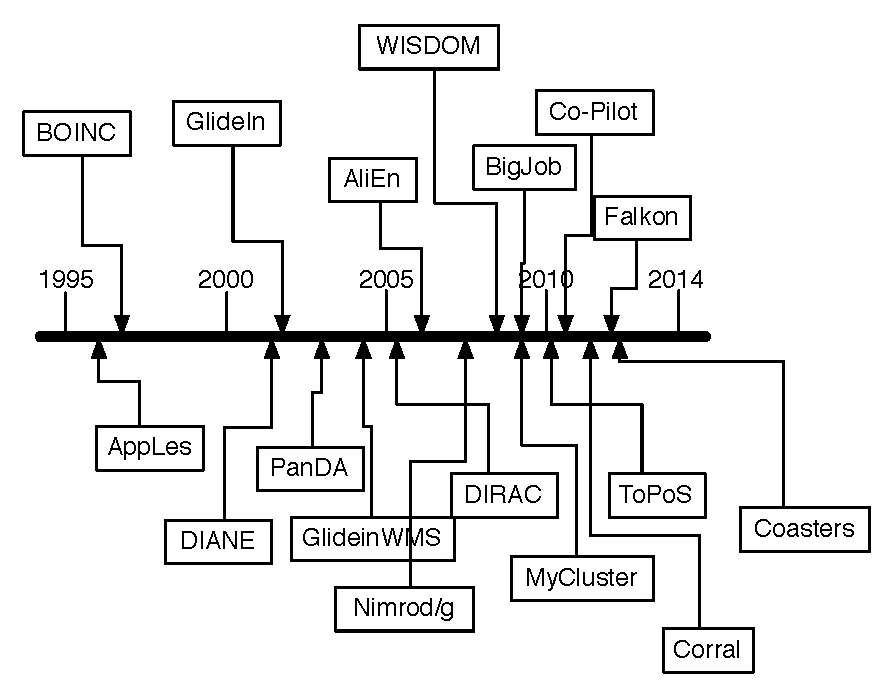
\includegraphics[width=0.45\textwidth]{figures/timeline}
    \caption{Introduction of systems over time. When available, the date of
    first mention in a publication or otherwise the release date of software
    implementation is used. \mtnote{Missing from from both Section 3 and 4:
    WISDOM, ToPoS, Corral. Missing from Section 3 but present in Section 4:
    MyCluster.}}
    \label{fig:timeline}
\end{figure}

\begin{figure}[t]
  \centering
    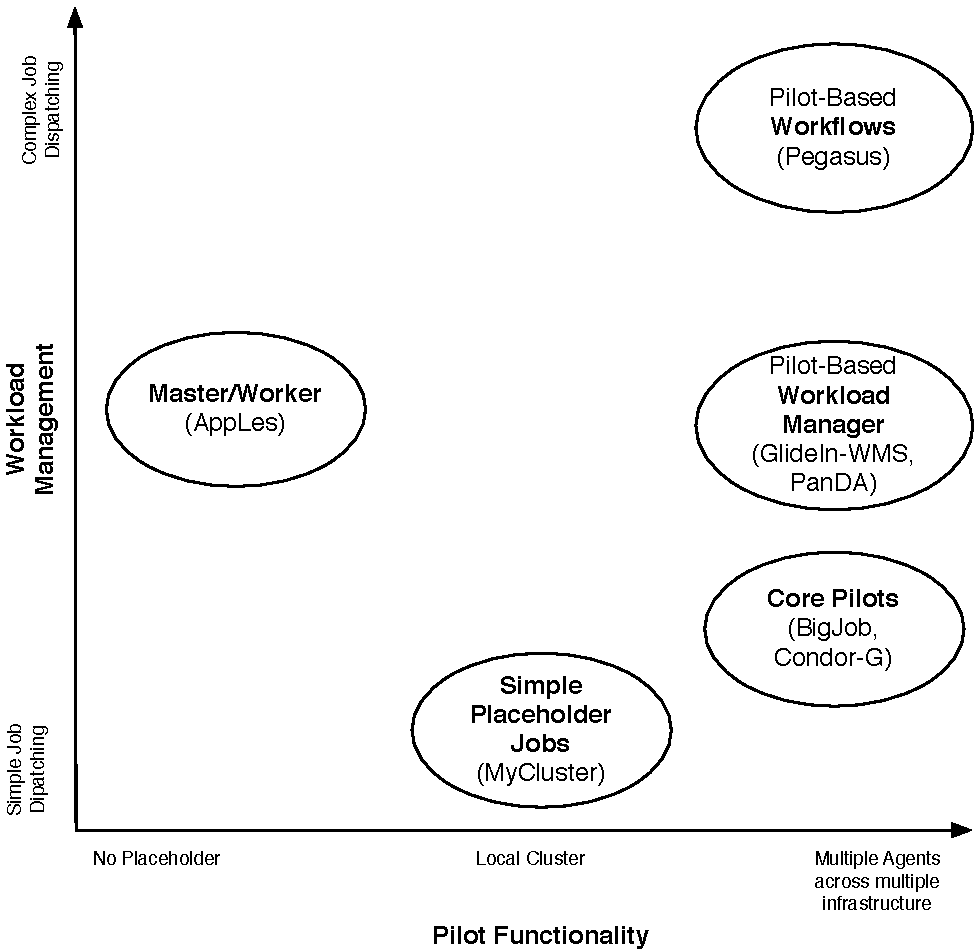
\includegraphics[width=.45\textwidth]{figures/pilotjob-clustering.pdf}
  \caption{Pilot-Job Clustering}
  \label{fig:pilotjob_clustering}
\end{figure}

AppLeS~\cite{Berman:1996:apples} is a framework for application-level scheduling
and offers an example of an early implementation of resource placeholder. AppLeS
provides an agent that can be embedded into an application thus enabling the
application to acquire resources and to schedule tasks onto these. Besides \MW,
AppLeS also provides application templates, e.\,g.\ for parameter sweep and
moldable parallel applications~\cite{Berman:2003:ACG:766629.766632}.

AppLeS offered user-level control of scheduling but did not isolate the
application layer from the management and coordination of task execution. Any
change in the coordination mechanisms directly translated into a change of the
application code. The next evolutionary step was to create a dedicated
abstraction layer between those of the application and of the various batch
queuing systems available at different remote systems.

Around the same time as AppLeS was introduced, volunteer computing projects
started using the \MW coordination pattern to achieve high-throughput
calculations for a wide range of scientific problems. The workers of these
systems could be downloaded and installed on the users workstation.
With an installation base distributed across the globe, workers pulled and
executed computation tasks when CPU cycles were available.

The volunteer workers were essentially heterogeneous and dynamic as opposed to
the homogeneous and static AppLeS workers. The idea of farming out tasks in a
dynamic distributed environment including personal computers promised to lower
the complexity of distributed applications design and implementation. Each
volunteer worker can be seen as an opportunistic resource placeholder and, as
such, an implementation of the core functionality of the \pilot abstraction.

The first public volunteer computing projects were The Great Internet Mersenne
Prime Search effort\cite{woltman:2004:gimps}, shortly followed by
distributed.net~\cite{Lawton:2000:distributednet} in 1997 to compete in the
RC5-56 secret-key challenge, and the SETI@Home project, which set out to
analyze radio telescope data. The generic BOINC distributed master-worker
framework grew out of SETI@Home, becoming the {\it de facto} standard framework
for voluntary computing~\cite{Anderson:2004:BSP:1032646.1033223}.

It should be noted that process of resource acquisition is different in AppLes
and voluntary computing. The former has prior knowledge of the available
resources while the latter has none. \jhanote{In the previous sentence, I think
adding ``prior'' in lieu of ``complete'' would be most effective.
OK?}\mtnote{Done.} As a consequence, AppLes can request and orchestrate a set of
resources, allocate tasks in advance to specific workers (i.e. resources
placeholders), and implement load balancing among resources. In voluntary
computing tasks are pulled by the clients when they become active and, as such,
specific resource availability is unknown in advance. This potential drawback is
mitigated by the redundancy offered by the large scale that voluntary computing
can reach thanks to its simpler model of worker distribution and installation.

% The opportunistic use of geographically distributed resources championed by
% voluntary computing offers several advantages. The resource landscape
% available for scientific research is fragmented across multiple institutions,
% managed with different policies and protocols, and heterogeneous both in
% quantity and quality. Once aggregated, the sum of otherwise limited resources
% can support very large distributed computations and a great amount of
% multi-tenancy. Note that given the required capabilities, this model of
% resource provisioning can still support the execution of parallel applications
% on the few resources that offer low-latency network interconnect.\msnote{This
% paragraph is a good candidate for removal?}

\jhanote{is ``batch'' redundant?} \mtnote{Probably
(based on: http://research.cs.wisc.edu/htcondor/doc/condor-practice.pdf). I
changed system to framework as system is used differently in the following
sentence.} Condor is a high-throughput distributed computing framework that uses
diverse and possibly geographically distributed resources~\cite{thain2005}.
Originally, Condor was created for systems within one administrative domain but
Flocking~\cite{Epema:1996:flocking} made it possible to group multiple Condor
resource pools in an aggregative manner. However, resource management required
system level software configurations that had to be made by the administrator of
each individual resource of each Condor resource pool.

% \jhanote{resource management could not be done on application level'' does not
%   make sense to me.  Are we referring to aggregation?}\mtnote{Better?}

This limitation was overcame by integrating a resource placeholder mechanism
within the Condor system. Condor-G/GlideIn~\cite{condor-g} allowed users to add
remote grid resources to Condor resource pools. In this way, users could
uniformly execute jobs on resource pools composed by diverse resources. Thanks
to its use of resource placeholders, GlideIn was one of the systems
pioneering the \pilot abstraction implementation, enabling some \pilot
capabilities also for third parties systems like Bosco~\cite{bosco}.

\jhanote{So we are sure flocking came before glide-in?} \mtnote{Mark?}
% \jhanote{Also there is a bit of care needed: we're implying glide-in is a
% resource placeholder -- which is part of a pilot, and not necessarily a full
% pilot.} \mtnote{We do not use \pilotjob system so I do not think we are implying
% that glideIn is a `full pilot' (even if I am not so sure what exactly a full
% pilot is). I slightly edited the sentence, any better?}

% \jhanote{as this is historical evolution, some parts need to be in the past
% tense. Care will be needed to get the tense right.} \mtnote{Better?}

The success of Condor-G/GlideIn shows the relevance of the pilot abstraction to
enable scientific computation at scale and on heterogeneous resources. The
implementation of GlideIn also highlighted at least two limitations: user/system
layer isolation, and application development model. While GlideIn allows for the
user to manage resource placeholders directly, daemons must still be running on
the remote resources. This means that GlideIn cannot be deployed without
involving the resource owners and system administrators. Implemented as a
service, GlideIn supports integration with distributed application frameworks
but does not programmatically support the development of distributed
applications by means of dedicated APIs and libraries.

The BigJob \pilotjob system~\cite{luckow2010} was designed to address these
limitations, to broaden the type of applications supported by the pilot-based
execution model, and to extend the \pilot abstraction beyond the boundaries of
compute tasks.  BigJob offers application-level programmability to provide the
end-user with more flexibility and control over the design of distributed
application and the isolation of the management of their execution. BigJob is
flexible and extensible and uses the Simple API for Grid Applications (SAGA)
interoperability library~\cite{saga-x,goodale2006,luckow2010} to work on a
variety of infrastructures.  Additionally, BigJob has also been extended to work
with data and, analogous to compute pilots, to abstract away direct user
communication between different storage systems.

% was recently re-implemented as a production-level tool named
% ``RADICAL-Pilot''~\cite{radical_pilot_paper}. rep- resents one of the latest
% evolutionary stages of the Pilot ab- straction. from an initial phase in which

% \msnote{The latter brings it back to the stage of apples, thats probably not
%   what we want to say ...}  \mtnote{Apologies, I am not sure I understand this
%   comment.}

BigJob was recently re-implemented as a production-level tool named
`RADICAL-Pilot''~\cite{review_rp-paper-2015}. BigJob/RADICAL-Pilot represent an
evolution of the \pilot abstraction: initially pilots were implemented as ad hoc
place holder machinery for a specific application but evolved to be integrated
with the middleware of remote resources. BigJob/RADICAL-Pilot implements the
\pilot abstraction as an interoperable compute and data management system that
can be programmatically integrated into end-user applications and thus provides
both features.

Another ongoing evolutionary trend has been to implement the \pilot abstractions
into pilot-based workload managers, thus moving away from providing simple
pilot capabilities in application space. These higher-level systems which are
often centrally hosted, move critical functionality from the client to the
server (i.e. a service model). These systems usually deploy pilot factories
that automatically start new pilots on demand and integrate security mechanisms
to support multiple users simultaneously.

Several of these have been developed in the context of the LHC experiment at
CERN, which is associated with a major increase in the uptake and availability
of pilots, e.\,g.\ DIANE~\cite{Moscicki:908910}, GlideInWMS,
DIRAC~\cite{1742-6596-219-6-062049}, \panda~\cite{1742-6596-331-7-072069},
AliEn~\cite{1742-6596-119-6-062012} and Co-Pilot~\cite{copilot-tr}. Each of
these \pilotjob systems serves a particular user community and experiment.
Interestingly, these systems are functionally very similar, work on almost the
same underlying infrastructure, and serve applications with very similar (if not
identical) characteristics.

% \jhanote{Need consistency between PanDA (two paras from now) and PanDa}

\mtnote{I would consider to cut the following 5 paragraphs. They are largely a
  repetition of what we have in 4.2 and historically they offer details that
  have been already summarized (or can be summarized) in the preceding,
  encompassing paragraph.}  \jhanote{I think this is a fair suggestion. But we
  need to ensure that those that are not discussed in 4.2 are in the paragraph
  ``for all other pilot systems'' --- so as to avoid possibly being dinged by a
  reviewer from that system..}\jhanote{I also note that GWPilot isn't referenced
  anywhere/anymore. We should be sure to put GWPilot into that paragraph}


GlideinWMS~\cite{1742-6596-119-6-062044} is a higher-level workload management
system that is based on the pilot capabilities of Condor GlideIn. The system
can, based on the current and expected number of jobs in the pool, automatically
increase or decrease the number of active Glide-ins (i.e. pilots) available to
the pool. GlideinWMS is a multi-user \pilotjob system commonly deployed as a
hosted service. GlideinWMS attempts to hide the pilot capabilities rather than
exposing them to the user. GlideinWMS is currently deployed in production on the
Open Science Grid (OSG)~\cite{url_osg} and is the recommended mode for new users
wanting to access OSG resources.

\panda (Production and Distributed Analysis)~\cite{1742-6596-331-7-072069} is
the workload management system of the ATLAS experiment, used to run managed
production and user analysis jobs on the grid. The ATLAS Computing Facility
operates the pilot submission systems. This is done using the \panda `AutoPilot'
scheduler component which submits pilot jobs via Condor-G. \panda also provides
the ability to manage data associated the jobs managed by the \panda workload
manager.

In addition to processing, AliEn~\cite{1742-6596-119-6-062012} also provides the
ability to tightly integrate storage and compute resources and is also able to
manage file replicas. While all data can be accessed from anywhere, the
scheduler is aware of data localities and attempts to schedule compute close to
the data. AliEn deploys a pull-based model~\cite{Saiz:2003:alien} assuming that
the resource pool is dynamic, and that a pull model doesn't require the broker
to keep detailed track of all resources, which leads to a more simple
implementation. \jhanote{what is the broker here?} \mtnote{Mark?}

DIRAC~\cite{1742-6596-219-6-062049} used by the LHCb experiment~\cite{lhcb} is
another comprehensive pilot-based workload management system.
It supports the management of data, which can be placed in different
kinds of storage elements (e.\,g.\ based on SRM).

Another interesting \pilotjob system that is used in the LHC context is
Co-Pilot~\cite{copilot-tr}. Co-Pilot serves as an integration point among
different grid \pilotjob systems (such as AliEn and \panda), clouds, and
volunteer computing resources. Co-Pilot provides components for building a
framework for seamless and transparent integration of these resources into
existing grid and batch computing infrastructures exploited by the High Energy
Physics community.

\mtnote{End of the suggested paragraph removal.}

The \pilot abstraction has also been integrated into scientific workflow
systems. \pilotjob systems have proven an effective tool for managing the
workloads executed in the various stages of a workflow. For the Pegasus
project\cite{deelman2015}, the Corral
system~\cite{Rynge:2011:EUG:2116259.2116599} was developed to support the
optimize the placements of pilots with respect to their workload for the
Pegasus workflow system. Corral serves as a front-end to Condor GlideIn. In
contrast to GlideinWMS, Corral provides more explicit control over the placement
and start of pilots to the end-user. Corral was later extended to also serve as
a possible front end to GlideinWMS.

Swift~\cite{Wilde2011} is a scripting language designed for expressing abstract
workflows and computations. The language also provides capabilities for
executing external application as well as the implicit management of data flows
between application tasks. Swift uses a \pilot implementation called
``Coaster''~\cite{coasters}, developed to address workload management
requirements by supporting various types of infrastructure, including clouds and
grids.

Swift has also been used in conjunction with Falkon~\cite{1362680}. Falkon was
engineered for executing many small tasks on HPC systems and shows high
performance compared to the native queuing systems. Falkon is a paradigmatic
example of how the \pilot abstraction can be implemented to support very
specific workload.

The proliferation of \pilotjob systems underlines not only a progressive
appreciation for the \pilot abstraction but also the emergence of a \pilot
paradigm to support the execution of distributed and increasingly of parallel
applications. The brief description of the many \pilotjob system implementations
introduced in this section helps to identify some distinctions in terms of
design, usage and operation modes. Figure~\ref{fig:pilotjob_clustering} is a
graphical representation of this rough clustering.

The evolution of the \pilot paradigm has been organic and uncoordinated leading
to an inconsistent terminology related to the \pilot abstraction, its
implementations and usage. A coherent understanding of the \pilot components and
functionalities is still missing leading to a blurred definition of \pilot
abstraction and how it should be distinguished from other abstractions and
middleware and application software.

The evolution of \pilots attests to their usefulness across a wide range of
deployment environments and application scenarios, but the divergence in
specific functionality and inconsistent terminology calls for a standard
vocabulary to assist in understanding the varied approaches and their
commonalities and differences. This is primary motivation of
Section~\ref{sec:understanding}.



%------------------------------------------------------------------------------
% SECTION 3
%------------------------------------------------------------------------------

\newcommand{\vocab}[1]{\textbf{#1}\xspace}
\newcommand{\prop}[1]{\textit{#1}\xspace}
\newcommand{\impterm}[1]{\texttt{#1}\xspace}

\section{Understanding the Landscape: Developing a Vocabulary}
\label{sec:understanding}

The overview presented in \S\ref{sec:history} shows a degree of heterogeneity
both in the functionalities and the vocabulary adopted by different \pilotjob
systems. Implementation details sometimes hide the functional commonalities and
differences among \pilotjob systems. Features and capabilities tend to be named
inconsistently, often with the same terms referring to multiple concepts or the
same concept named in different ways.

This section offers a description of the logical components and functionalities
shared by every \pilotjob system. The goal is to offer a paradigmatic
description of a \pilotjob system and a well-defined vocabulary to reason about
such a description and, eventually, about its multiple implementations.

% \jhanote{would ``description'' be better than ``analysis'' in the first
%   sentence?}

%------------------------------------------------------------------------------
% 3.1
\subsection{Logical Components and Functionalities}
\label{sec:compsandfuncs}

All \pilotjob systems introduced in~\S\ref{sec:history} are engineered to allow
for the execution of multiple types of workloads on machines with diverse
middleware, e.g. grid, cloud, or HPC. This is achieved in different ways,
depending on use cases, design and implementation choices, but also on the
constraints imposed by the middleware and policies of the targeted machines. The
common denominators among \pilotjob systems are defined along three dimensions:
purpose, logical components, and functionalities.

The purpose shared by every \pilotjob system is to improve workload execution when
compared to executing the same workload directly on one or more
resources. Performance of workload execution is usually measured by throughput
and execution time to completion, but other metrics could also be
considered: energy efficiency, data transfer minimization, scale of the workload
executed, or a mix of them. Metrics that are not performance related include
reliability, ease of application deployment and generality of workload.  In
order to achieve the required metrics under given constraints, each \pilotjob
system exhibits characteristics that are both common or specific to one or more
implementations. Discerning these characteristics requires isolating the minimal
set of logical components that characterize every \pilotjob system.

At some level, all \pilotjob systems employ three separate but coordinated
logical components: a \vocab{Pilot Manager}, a \vocab{Workload Manager}, and a
\vocab{Task Manager}. The Pilot Manager handles the description, instantiation,
and use of one or more resource placeholders (i.e. `pilots`) on single or
multiple machines. The Workload Manager handles the scheduling of one or more
workloads on the available resource placeholders. The Task Manager takes care of
executing the tasks of each workload by means of the resources held by the
placeholders.

The implementation details of these three logical components vary significantly
across \pilotjob systems (see~\S\ref{sec:analysis}). 
% One or more logical components may be responsible for specific
% functionalities, both on application as well as machine level;
For example, two or more logical components may be implemented by a single
software module or additional functionalities may be integrated into the three
managers. Nevertheless, the \pilot, Workload, and Task Managers can always be
distinguished across different \pilotjob systems.

% \jhanote{Should we use ``execution of tasks'' in opening sentence. We talk about
%   executing tasks before and after, and not necessarily workloads.  Issue of
%   consistency and granularity and not of correctness.} \mtnote{I reread from the
%   beginning and I think we use workload and task consistently: ``All \pilotjob
%   systems introduced in~\S\ref{sec:history} are engineered to allow for the
%   execution of multiple types of workloads'', ``The purpose shared by every
%   \pilotjob system is to improve workload execution'', ``The Workload Manager
%   handles the scheduling of one or more workloads'', ``The Task Manager takes
%   care of executing the tasks of each workload''}

Each \pilotjob system supports a minimal set of functionalities that allow for
the execution of workloads: \vocab{Pilot Provisioning}, \vocab{Task
  Dispatching}, and \vocab{Task Execution}. \pilotjob systems need to schedule
resource placeholders on the target machines, schedule tasks on the available
placeholders, and then use these placeholders to execute the tasks of the given
workload. More functionalities might be needed to implement a production-grade
\pilotjob system: authentication, authorization, accounting, data management,
fault-tolerance, or load-balancing. While these functionalities may be critical
implementation details, they depend on the specific characteristics of the given
use cases, workloads, or targeted resources. As such, these functionalities
should not be considered necessary characteristics of a \pilotjob system.

Among the core functionalities that characterize every \pilotjob system, Pilot
Provisioning is essential because it allows for the creation of resource
placeholders. As seen in \S\ref{sec:history}, this type of placeholder enables
tasks to utilize resources without directly depending on the capabilities
exposed by the target machines. Resource placeholders are scheduled onto target
machines by means of dedicated capabilities, but once scheduled and then
executed, these placeholders make their resources directly available for the
execution of the tasks of a workload.

% \jhanote{possibly use ``resources'' in lieu of remote machines?} \mtnote{Would
%   that overload the term with two separate meanings: resource as what is held
%   and resource as DCR?}\jhanote{I removed ``remote'', retained machine.  I want
%   to avoid implying placeholders have to be distributed from the point of
%   submission.} \mtnote{Great.}

% \jhanote{We may want to introduce the vocabulary of resource/DCR/DCI that we
%   developed for the proposals here, and make it consistent throughout the
%   paper. In this para for example we use the term DCI resource, which is
%   inconsistent with developed vocabulary} \mtnote{If we want the definitions
%   here, then we should probably move all of them before this subsection. Do
%   you want me to do it? Meanwhile, I rephrased the whole subsection avoiding
%   DCI altogether and added the definition of DCR to the next subsection.}

% MS: I would move this comment to section 5 I think, as multi-tenant pilot
% systems do have to make these trade-offs, and it would be good to point that
% out. (not doing it now because of MT lock in 5) Furthermore, resource
% placeholders are logical partitions of resources that do not need to leverage
% trade-offs among competing user requirements as needed instead with large
% pools of resources adopting multi-tenancy.

The provisioning of resource placeholders depends on the capabilities exposed by
the middleware of the targeted machine and on the implementation of each \pilot
system. Typically, for middleware adopting queues, batch systems, and
schedulers, provisioning a placeholder involves it being submitted as a job.
For such middleware, a `job' is a type of logical container that includes
configuration and execution parameters alongside information on the application
to be executed on the machine's compute nodes. Conversely, for
infrastructures that do not adopt a job-based middleware, a resource placeholder
would be executed by means of other types of logical container as, for example,
a virtual machine or a Docker Engine~\cite{bernstein2014,felter2014}.

\mtnote{Too many execut*. Should we use `code' instead of `executable'? Any
  better option than `code' to replace `executable'?} \jhanote{used application, but
  task might be better? code is acceptable too.}

Once resource placeholders are bound to the resources of a machine, tasks need
to be dispatched to those placeholders for execution. Task dispatching does not
depend on the functionalities of the targeted machine's middleware so it can be
implemented as part of the \pilotjob system. In this way, the control over the
execution of a workload is shifted from the machine's middleware to the \pilot
system. This shift is a defining characteristic of the \pilot paradigm, as it
decouples the execution of a workload from the need to submit its tasks via the
machine's scheduler.  For example, the execution of tasks of a workload will not
individually depend upon the specifics of the targeted machine's state or
availability, but rather on those of the placeholder.
% For example, the tasks of a workload will not individually
% have to wait on the targeted machine's queues, but rather on the availability of
% the placeholder before being executed.
More elaborate execution patterns involving task and data interdependence can
thus be implemented independent of the target machine's middleware
capabilities. Ultimately, this is how \pilotjob systems allow for the direct
control of workload execution and the optimization, for example, of execution
throughput.

% \jhanote{Matteo: please confirm you are OK with the suggested change.} \mtnote{I
%   like the generality of the new version. Would this improve readability: ``For
%   example, the execution of tasks of a workload will not individually depend
%   upon the specifics of the targeted machine's state or availability, but rather
%   on those of the placeholder.''?}

% \jhanote{I'd like to use a more general term than ``machine's scheduler'' when
%   talking about the defining characteristic. It weakens the punch of an
%   impactful and important sentence.}  \mtnote{Any idea about what term would
%   you like to use?}  \jhanote{Also in the subsequent sentence, ``The tasks of
%   a workload..''. I've introduced a for example to help give a specific
%   instance of the general paradigm.} \mtnote{OK.}

Communication and coordination are two distinguishing characteristics of
distributed systems and \pilotjob systems are no exception. The three logical
components -- Workload Manager, Pilot Manager, and the Task Manager -- need to
communicate in order to coordinate the execution of the given workload on the
instantiated resource placeholders.  Nonetheless, \pilotjob systems are not
defined by any specific communication pattern and coordination approach. The
logical components of a \pilotjob system may communicate using any suitable
pattern (e.g. one-to-one, many-to-one, one-to-many~\ref{comm_patterns} with a
push or pull model), or coordinate adopting any suitable mechanism (e.g. time
synchronization, static or dynamic coordinator election, local or global
information sharing, or \MW). The same applies to network architectures and
protocols: different network architectures and protocols may be used to achieve
effective communication and coordination.
% \jhanote{is this a reference to coordination or communication? unclear}
% \mtnote{`communication and coordination' so I would say to both.}

As seen in~\S\ref{sec:history}, \MW is a very common coordination pattern among
\pilotjob systems. When the master is identified with the Workload Manager, and
the worker with the Task Manager, the functionalities related to task
description, scheduling, and monitoring will generally be implemented within the
Workload Manager, while the functionalities needed to execute each task will be
implemented within the Task Manager. Alternative coordination strategies, for
example, where a Task Manager directly coordinates the task scheduling, might
require a functionally simpler Workload Manager but a comparatively more
feature-rich Task Manager. The former would require capabilities for submitting
tasks, while the latter capabilities to coordinate with its neighbor executors
leveraging, for example, a dedicated overlay network. While these systems would adopt
different coordination strategies, they could be both be considered \pilotjob
systems.

Data management can play an important role within a \pilotjob system. For
example, functionalities can be provided to support the local or remote data
staging required to execute the tasks of a workload, or data might be managed
according to the specific capabilities offered by the targeted machine's
middleware. How these requirements are implemented do not
define a core functionality of the \pilot system.
%For example,
%\pilotjob systems can be devised in which tasks do not require any data
% management because they: (i) do not necessitate input files; (ii) do not produce
% output files; (iii) data is already locally available; or (iv) data management
% is outsourced to third-party systems.
Being able to read and write files to a local filesystem should then be
considered the minimal capability related to data required by a \pilotjob
system. More advanced and specific data capabilities like, for example, data
replication, (concurrent) data transfers, data abstractions other than files and
directories, or data placeholders should be considered special-purpose
capabilities, not characteristic of every \pilotjob system.  \jhanote{Please
  check my edit/deletion. I did not think the statement and listing of ``tasks
  not requiring data management helped in anyway''} \mtnote{That
  (over)specification was due to the endless debate about the idea that data
  management is not a necessary functionality of \pilot systems. If we think
  that we drive the point clearly enough then I would eliminate the statement
  and listing. On the other hand, if we think this could be a point of
  `conceptual friction' for the readers, I would keep the point
  over-specified.}\jhanote{OK, lets keep this open for the moment and decide in
  the next iteration}

In the following sub-section, a minimal set of terms related to the logical
components and capabilities described so far is defined.

%------------------------------------------------------------------------------
% 3.2
\subsection{Terms and Definitions}
\label{sec:termsdefs}

% \jhanote{Is the second sentence OK?} \mtnote{Superfluous? I commented it out but
% happy to bring it back modified if you think it is needed.}
% It is the case that \pilotjob systems are commonly referred to as
% `\pilotjob systems', a clear indication of the primary role played by the
% concepts of `pilot' and `job' in this type of system.

The terms `pilot' and `job' are arguably among the most relevant when referring
to \pilotjob systems. The definition of both concepts is context-dependent and
several other terms need to be clarified in order to offer a coherent
terminology. Both `job' and `pilot' need to be understood in the context of
machines and middleware used by \pilotjob systems. These machines offer compute,
storage, and network resources and \pilots allow for the users to utilize those
resources to execute the tasks of one or more workloads.

\begin{description}

\item[Task.] A container for operations to be performed on a computing
platform, alongside a description of the properties of those operations, and
indications on how they should be executed. Implementations of a task may
include wrappers, scripts, or applications.

\item[Workload.] A set of tasks, possibly related by a set of arbitrarily
complex relations.

\item[Resource.] Finite, typed, and physical quantity utilized when executing
the tasks of a workload. Compute cores, data storage space, or network
bandwidth between a source and a destination are all examples of resources
commonly utilized when executing workloads.

\item[Distributed Computing Resource (DCR).] A set of machines characterized by
  a tuple: \{a set of possibly heterogeneous resources, a middleware software,
  and an administrative domain\}. \mtnote{I used `set of machines' because from
    now on we use DCR instead of machine and I think we need to link explicitly
    the two.  Would you agree?}\jhanote{would it then not be Distributed
    Computing Resources?}

\end{description}

A cluster is a typical example of DCR: it offers compute and data resources; it
exposes an access middleware, for example, the Torque batch system, the Globus
grid middleware, of the OpenStack platform; and it is deployed by and consistent with the policies of an
administrative domain like, for example, XSEDE or a certain University.

As seen in~\S\ref{sec:history}, most of the DCRs used by \pilotjob systems
utilize `queues', `batch systems', and `schedulers'. In such DCRs, jobs are
scheduled and then executed by a batch system.

\begin{description}

\item[Job.] Functionally defined as a `task' from the perspective of the DCR,
but in the case of a \pilotjob system indicative of the type of container
required to acquire resources on a specific infrastructure.

\end{description}

When considering \pilotjob systems, jobs and tasks are functionally analogous
but qualitatively different. Functionally, both jobs and tasks are containers --
i.e. metadata wrappers around one or more executables often called `kernel',
`application', or `script' \mtnote{If we are going to use `code' instead of
  `executable' in the previous subsection, I would add `code'
  here.}. Qualitatively, the term `task' is used when reasoning about workloads,
while `job' is used in relation to a specific type of DCR middleware where such
a container is submitted. Accordingly, tasks are considered as the functional
units of a workload, while jobs as a way to schedule one or more tasks on a DCR
with a specific middleware.  It should be noted that, given their functional
equivalence, the two terms can be adopted interchangeably when considered
outside the context of \pilotjob systems. Indeed, workloads are encoded into
jobs when they have to be directly executed on DCRs that support or require that
type of container.

% \jhanote{minor nitpic: are we assuming 1 task per job? I don't think we
%   should..} \mtnote{I do not think we are assuming a 1:1 relation as we use
%   `tasks'. Should we make it explicit?}\jhanote{Yes, if only to say there is no
%   relationship} \mtnote{Better?}

% \jhanote{maybe workload in lieu of container in the previous
%   sentence?}\mtnote{The idea is that job is dependent from a middleware,
%   specifically a HPC-based one. For example, we do not submit a `job' to a cloud
%   middleware. I replaced `executed' by `submitted'.  Any better?}

% \jhanote{We start with jobs and tasks, but it gets a bit tricky to navigate this
%   past paragraph, because workloads, tasks and jobs are discussed. Would it be
%   better if the mapping in this paragraph was between tasks and jobs only? or
%   just workloads and jobs?} \mtnote{I do not think I would be able to remove
%   workload from the previous paragraph as it is used to distinguish
%   qualitatively jobs from tasks. Maybe the distinction is not
%   convincing?}\jhanote{it reads ok now. simplifying made it smoother}

As described in~\S\ref{sec:compsandfuncs}, a resource placeholder needs to be
submitted to a DCR wrapped in the type of container supported by the middleware
of that specific DCR. For this reason, the capabilities exposed by the job
submission system of the target DCR determine the submission process of resource
placeholders and its specifics.  For example, when wrapped within a `job',
placeholders are provisioned by submitting a job to the DCR queuing system, and
become available only once the job has been scheduled, and only for the duration
of the job lifetime.

% \jhanote{changed DCI to DCR. OK?}\jhanote{not sure what ``out of the queue''
%   means? maybe say, ``.. become available when the job is active, and is
%   available...''} \mtnote{Better? I used `once... has become' to indicate that
%   the job sits within the queue for a certain amount of time.}


% For example, for a DCR exposing a HPC or grid
% middleware~\cite{HPC_grid_middleware}, a resource placeholder needs to be
% wrapped within a `job'. For other type of middleware, the same resource
% placeholder will need to be wrapped within a different type of container as,
% for example, a VM or a Docker Engine.

A \pilot is a resource placeholder. As a resource placeholder, a pilot holds
portion of a DCR's resources for a user or a group of users, depending on
implementation details. A \pilotjob system is software capable of creating
pilots so as to gain exclusive control over a set of resources on one or more
DCRs and then to execute the tasks of one or more workloads on those pilots.


% \jhanote{also I would not use the word exclusive} \mtnote{Why?}\jhanote{In our
%   definition of Resource earlier in this section, we define it as a finite
%   physical quantity utilized. As we do not claim that the resource is logical we
%   should not claim that the resource is exclusively available}\mtnote{Thank you.
%   I think exclusive applies because once the quantity of resource is held by the
%   pilot, it can be used only by the pilot. For example, it is not shared with
%   the DCR scheduler as other jobs of the DCR cannot use those
%   resources.}\jhanote{I will let it go, but the point about ``resource'' not
%   being a logical entity remains important. If it is not logical, it is not
%   possible to say that another job is not using that resource or that resource
%   is not doubly provisioned.}


\begin{description}

\item[Pilot.] A container (e.g., a `job') that functions as a resource
placeholder on a given infrastructure and is capable of executing tasks of a
workload on that resource.

\end{description}

It should be noted that the term `pilot' as defined here is named differently
across \pilotjob systems. Depending upon context, in addition to the term
`placeholder', pilot may also be named `agent' or
`\pilotjob'~\cite{moscicki2011,pinchak2002}. All these terms are, in practice,
used as synonyms without properly distinguishing between the type of container
and the type of executable that compose a pilot. This is a clear indication of
how necessary the minimal and consistent vocabulary offered here is when
reasoning analytically about multiple \pilotjob system implementations.

Until now, the term \pilotjob system has been used to indicate those systems
capable of executing workloads on pilots. From now on, the term `\pilot system'
will be used instead, as the term `job' in `pilot-job' identifies just the way
in which a pilot is provisioned on a DCR exposing specific capabilities; it is
not a general property of all the \pilotjob systems. The use of the term
`\pilotjob system' should therefore be regarded as a historical artifact, viz.,
the targeting of a specific class of DCRs in which the term `job' was, and still
is, meaningful. With the development of new types of DCR middleware as, for
example, those based on virtual machines, the term `job' has become too
restrictive, a situation that can lead to terminological and conceptual
confusion.

\mtnote{nitpick: `those based on virtual machines' does not exclude jobs and schedulers. For example, Nimbus or the CNAF `cloud' use queues and jobs to instantiate VMs.}

% \jhanote{I removed VMs to be a bit more specific}

% \jhanote{even by my standards of repeating the main points, i think we are
% painfully belabouring the point about ``jobs'' in pilot-jobs.} \mtnote{Maybe so
% but I do not see where we explicitly say this before. I have eliminated an
% example in which we were repeating the concept of job as a type of container.
% Here we make the case of a terminological confusion. Any better?}

We have now defined resources, DCRs, and pilots. We have established that a
pilot is a placeholder for a set of resources. When combined, the resources of
multiple pilots form a resource overlay. The pilots of a resource overlay can
potentially be distributed over multiple and diverse DCRs.

\mtnote{We may want to use resource overlay in Section 4.3 when we describe multi-DCR, multi-pilot scenarios.}

% The details of this aggregation or federation is outside the scope of this
% paper.

\begin{description}
\item[Resource Overlay.] The aggregated set of resources of multiple pilots.
\end{description}

Three more terms associated with \pilot systems need to be explicitly defined:
`Multi-level scheduling', `early binding', and `late binding'.

% \jhanote{should we use lower case for second instance of ``pilots'' ? This would
%   make it consistent with job, task, workload as these are now simply similar
%   elements of our vocabulary?} \mtnote{This has opened the proverbial can of
%   warms. Ongoing but will need revision.}

\jhanote{In case it suggests a change in the wording of opening sentence (and as
  discussed after the definition of multi-level scheduling downstream in this
  sub-section): the same entity can be scheduled at multiple levels, different
  entities can be scheduled at the same or different levels. These have all
  historically be clubbed as multi-level scheduling, i.e., there is multi-level
  and dimensional scheduling. Not sure if want to make distinction explicit
  here.} \mtnote{I am not sure I follow. We may want to discuss this on a call/meeting.}

Pilot systems are said to implement multi-level scheduling because they require
the scheduling of two types of entities: pilots and tasks. A portion of the
resources of a DCR is allocated to one or more pilots, and the tasks of a
workload are dispatched for execution to those pilots. As alluded to in the
previous sub-section, this is a fundamental feature of \pilot systems.  It leads
to the following: (i) more flexible and potentially reduced times to completion
of workloads as a consequence of avoiding a centralized job management system
multiple times; and (ii) the tasks of a workload can be bound to a set of pilots
before or after it becomes available on a remote resource. Depending on the
implementation of a \pilot system, there can be another level of scheduling,
where the \pilot system makes scheduling decisions about task placement within
the pilot's resource allocation.


% \jhanote{about point (i): I know we caveat the statement with
%   ``potentially'' but maybe the focus should be on (a) greater control to the
%   user without any increase in burden/complexity or compromise in performance?}

% \jhanote{I don't think it is about simplification (that is doubtful). It is
%   about greater control as a consequence}

The greater control obtained as a consequence of removing the dependence of
every task on the job submission system of the DCR is one of the main reasons
for the success and early adoption of \pilot systems. As mentioned
in~\S\ref{sec:compsandfuncs}, the tasks of a workload can be executed on a pilot
without each task individually waiting in the queuing system of the DCR's
middleware. This greater control results in several advantages, including
possibly increasing the throughput of the workload execution, and reusing active pilots to execute multiple workloads. How tasks are actually scheduled to pilots is a matter of
implementation. For example, a dedicated scheduler could be adopted, or tasks
might be directly scheduled to a pilot by the user.

The type of binding of tasks to pilots depends on the state of the pilot. A
pilot is inactive until it is executed on a DCR, is active thereafter, until it
completes or fails. Early binding indicates the binding of a task to an
inactive pilot; late binding the binding of a task to an active one. Early
binding is potentially useful to increase the information about which pilots
can be deployed: by knowing in advance the properties of the tasks that are
bound to a pilot, specific deployment decisions can be made for that pilot.
Additionally, in case of early binding, other type of decisions related to the
workload could be made, e.g., the transfer of data to a certain resource while
the pilot is still inactive. Late binding is instead critical to assure the
aforementioned high throughput of the distributed application by allowing
sustained task execution without additional queuing time or container
instantiation time.

Some aspects of early binding can also be achieved without a \pilot system, but,
importantly, \pilot systems permit both types of binding, even within a single
workload.

% \jhanote{Is both a reference to early and late binding?} \mtnote{I would think
%   so. Any better?  Should we just delete the whole three lines?}

% \msnote{I would think parts of this paragraph also have their place in S5 (if
% its not already there)}
% \mtnote{The notion of binding needs to be fully understood before getting into
% 4. I would leave this as it is here but I am open to discuss about it.}
% \msnote{Agreed, with 'also' I meant repeating, not moving}

\begin{description}

\item[Multi-level scheduling.] Scheduling pilots onto resources, and
scheduling tasks onto (active or inactive) pilots.

\item[Early binding.] Binding one or more tasks to an inactive pilot.

\item[Late binding.] Binding one or more tasks to an active pilot.

\end{description}

%\jhanote{everything after here till the end of section 3 needs work.}

% \definecolor{term}{RGB}{153,39,38}
% \definecolor{funct}{RGB}{0,128,64}
% \definecolor{lcomp}{RGB}{0,128,255}

% \begin{table*}
%  \centering
%  \begin{tabular}{|p{4cm}|p{3.2cm}|p{3.2cm}|}
%   \hline
%     \textbf{Term} &
%     \textbf{Functionality} &
%     \textbf{Logical Component} \\
%   \hline
%   \hline
%     \textcolor{term}{Workload} &
%     \textcolor{funct}{Task Dispatching} &
%     \textcolor{lcomp}{Workload Manager} \\
%   \hline
%     \textcolor{term}{Task} &
%     \textcolor{funct}{Task Dispatching} \newline
%       \textcolor{funct}{Task Execution} &
%     \textcolor{lcomp}{Workload Manager} \newline
%       \textcolor{lcomp}{Task Manager} \\
%   \hline
%     \textcolor{term}{Resource} &
%     \textcolor{funct}{Pilot Provisioning} &
%     \textcolor{lcomp}{Pilot Manager} \\
%   \hline
%     \textcolor{term}{Infrastructure} or \textcolor{term}{DCI} &
%     \textcolor{funct}{Pilot Provisioning} &
%     \textcolor{lcomp}{Pilot Manager} \\
%   \hline
%     \textcolor{term}{Job} &
%     \textcolor{funct}{Pilot Provisioning} &
%     \textcolor{lcomp}{Pilot Manager} \\
%   \hline
%     \textcolor{term}{Pilot} &
%     \textcolor{funct}{Pilot Provisioning} \newline
%       \textcolor{funct}{Task Execution} &
%     \textcolor{lcomp}{Pilot Manager} \newline
%       \textcolor{lcomp}{Task Manager} \\
%   \hline
%     \textcolor{term}{Multi-level scheduling} &
%     \textcolor{funct}{Pilot Provisioning} \newline
%       \textcolor{funct}{Task Dispatching} &
%     \textcolor{lcomp}{Pilot Manager} \newline
%       \textcolor{lcomp}{Workload Manager} \\
%   \hline
%     \textcolor{term}{Early binding} &
%     \textcolor{funct}{Task Dispatching} \newline
%       \textcolor{funct}{Pilot Provisioning} &
%     \textcolor{lcomp}{Workload Manager} \newline
%       \textcolor{lcomp}{Pilot Manager} \\
%   \hline
%     \textcolor{term}{Late binding} &
%     \textcolor{funct}{Task Dispatching} \newline
%       \textcolor{funct}{Pilot Provisioning} &
%     \textcolor{lcomp}{Workload Manager} \newline
%       \textcolor{lcomp}{Pilot Manager} \\
%   \hline
%  \end{tabular}
%  \caption{\textbf{Mapping of the core terminology of \pilot systems into the
%      functionalities and logical components described in
%      \S\ref{sec:compsandfuncs}.}
%    \mtnote{Done in the text. Is it enough?}\msnote{Even with the
%      fancy colors ;-) I still fail to see the value of this table. Given that
%      I've become more appreciative of Fig4, I'm tempted to say that the figure
%      captures the multi-dimensionality much better than the table. Will
%      even volunteer to make it happen.}\jhanote{this table should either get a
%      major attention or it should simply be removed. It is unhelpful at best}}
%  \label{table:terminology}
% \end{table*}

% Table~\ref{table:terminology} offers an overview of the defined minimal and
% consistent vocabulary. The terms are mapped into the logical components of a
% \pilot system based upon .... \jhanote{Matteo: please finish the sentence}.
% The terms are also mapped onto minimal set of functionalities as defined
% in~\S\ref{sec:compsandfuncs} based upon .... \jhanote{Matteo: please finish
% the sentence}.

Figure~\ref{fig:core_vocabulary} offers a diagrammatic overview of the logical
components of \pilot systems (green) alongside their functionalities (blue) and
the defined vocabulary (red). An application submits a workload composed of
tasks to the \pilot system via an interface (a). The Pilot Manager is
responsible for pilot provisioning (b), the Workload Manager to dispatch tasks
to the Task Manager (c), the Task Manager to executes those tasks once the pilot
has become available (d). Figure~\ref{fig:core_vocabulary} shows not only the
separation between the DCR and the \pilot system but also how the resources on
which tasks are executed, are contained within different logical and physical
components. Appreciating the characteristics and functionalities of a
\pilot system depends upon understanding the levels at which each of
its component exposes capabilities.

% \jhanote{adequate paragraph. please don't say Figure 4(a) or Figure 4(b) as that
%   is canonically used for different sub-figures. maybe just (a) (or A, or 1)?}
%   \mtnote{Better?}

% \jhanote{``The same mapping'' is unclear.}
% \jhanote{Please describe figure 4 using at least 1 paragraph. Its a complex
%   figure and without a detailed description it is not going to help the
%   reader.}

Note how in Figure~\ref{fig:core_vocabulary}, scheduling happens at the DCR
level, for example by means of a cluster scheduler, and then at the pilot level.
The term `multi-level scheduling' pertains to both the pilot and workload
managers and their respective pilot provisioning and task dispatching
functionalities. \mtnote{Check Upper/lower case in the previous sentence of
managers and functionalities} As such, multi-level scheduling applies to two
different entities: jobs on DCR middleware, and tasks on pilots.

% \jhanote{are we also trying to say that multi-level scheduling is for different
%   ``entities'' at the different levels? either way, we may consider making that
%   explicit.}\mtnote{Better?}

Figure~\ref{fig:core_vocabulary} also helps to appreciate the critical
distinction between the container of a pilot and the pilot itself. A container,
for example a job, is used by the pilot manager to provision the pilot. Once the
pilot has been provisioned, it is the pilot and not the container that is
responsible of both holding a set of resources and offering the functionalities
of the task manager.

% \jhanote{How Table 1 helps is not at all clear/obvious. Hence I have removed a
%   reference to Table 1 in the opening of this sentence}.

Figure~\ref{fig:core_vocabulary} should not be confused with an architectural
diagram. No indications are given about the interfaces that should be used, how
the logical component should be mapped into software modules, or what type of
communication and coordination protocols should be used among such components.
This is why no distinction is made diagrammatically between early and late
binding.

% \jhanote{this is not needed here. we have discussed the difference between
%   early versus later before. by having it here we are losing the opportunity
%   to close out section 3 with the main lessons learnt} Their difference is
%   temporal and, as such, it can be highlighted only when describing the
%   succession of the states and operations of a \pilot system implementation.
%   In the early case, the binding of the tasks to a pilot will happen before
%   the submission of such a \pilot to the remote infrastructure. In the late
%   case, the binding will happen once the pilot has been instantiated and holds
%   already its resources.

\begin{figure}[t]
    \centering
        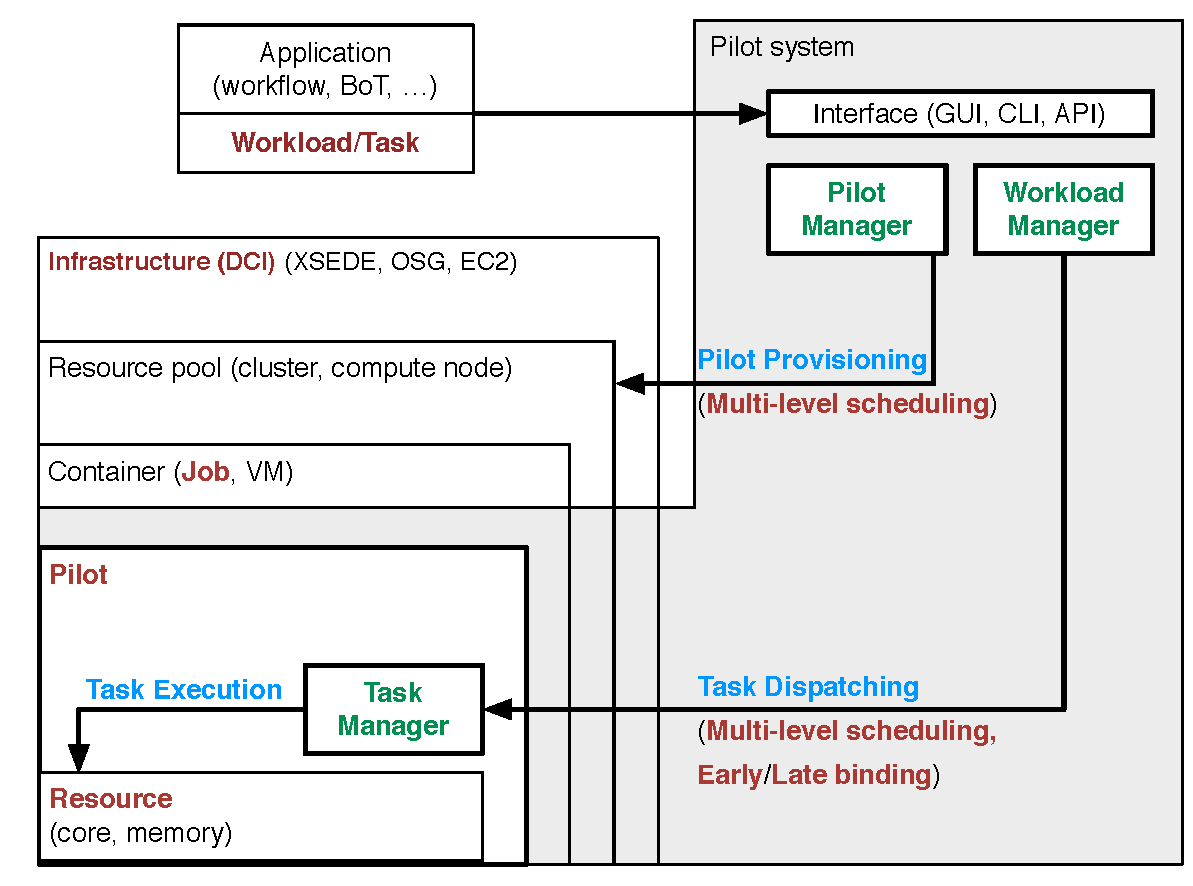
\includegraphics[width=.48\textwidth]{figures/core_vocabulary.pdf}
    \caption{Diagrammatic representation of the logical components,
    functionalities, and core vocabulary of a \pilot system. The terms of the
    core vocabulary are highlighted in red, those of the logical components of
    a \pilot system in green, and those of their functionalities in blue.}
    \label{fig:core_vocabulary}
\end{figure}

\mtnote{Lessons learned to be discussed before writing them down
  here.}\jhanote{do you mean ``here''?} \mtnote{As in: at this point of the
  subsection. Reading the whole Section in a go I am wondering whether we need
  to add more. The paragraph describing Figure~\ref{fig:core_vocabulary} seems
  to offer a summary of the main contributions and we have discussed
  contentious points along the way. }

The wide spectrum of available implementations of the logical components of a
\pilot system is explored in the next section.

% \mtnote{For S3, the TODO list is: 1. Argue explicitly that the offered `model'
% is sufficient and necessary in order to discriminate between \pilot and
% not-\pilot systems;} \mtnote{This is still somewhat an open issue.}


%------------------------------------------------------------------------------
% SECTION 4
%------------------------------------------------------------------------------
\section{Pilot Systems: Analysis and Implementations}
\label{sec:analysis}

Section \S\ref{sec:understanding} offered two main contributions: (i) the
minimal sets of logical components and functionalities of \pilot systems; and
(ii) a well-defined core terminology to support reasoning about such systems.
The former defines the necessary and sufficient requirements for a software
system to be a \pilot system, while the latter enables consistency when
referring to different \pilot systems. Both these contributions are used in this
section to analyze a selection of \pilot systems.

%that have seen significant
%implemented to execute real-life scientific workloads.

The goal of this section is twofold. Initially, the \pilot functionalities
presented in~\S\ref{sec:compsandfuncs} are used as the basis to infer core and
auxiliary \pilot implementation properties. Subsequently, a selection of \pilot
systems are analyzed and then clustered around the properties previously
defined. In this way, insight is offered about how \pilot systems are designed
and engineered, and the design principles that underly such systems.

% how to choose a \pilot system based on functional requirements,

\mtnote{The promises made at the end of these paragraph need to the fulfilled by
  offering remarks about: (i) choosing a pilot system; (ii) critical notes on
  the design and engineering of pilot systems; (iii) shared design
  principles. Should we do at the end of 4.2 or in 5?} \jhanote{I propose
  5. We'll also need to weaken the claims made at the end of the previous
  section.}

% -----------------------------------------------------------------------------
% 4.1
%
\subsection{Core and Auxiliary Properties}
\label{sec:properties}

This subsection analyzes the properties of diverse implementations of a \pilot
system. Two sets of properties are introduced: core and auxiliary (see
Table~\ref{table:property_component_mapping}). Both sets of properties are
chosen by considering the implementation requirements of the \pilot capabilities
as defined in~\S\ref{sec:history}. Core properties are necessary for every
\pilot system implementation to provide the minimal set of functionalities as
described in~\S\ref{sec:compsandfuncs}. Auxiliary properties are instead
required only as a support to the implementation of core properties. For
example, while every \pilot system has to implement a mechanism for pilot
instantiation, a specific authentication and authorization protocol may be
required to support the instantiation of pilots for a particular middleware of
a DCR. As such, auxiliary properties are not necessarily shared among all \pilot
systems.

% \jhanote{removed table reference..as a consequence of changes in 3, broken
%   reference here}

% \jhanote{there is a potential problem here: we define core property based upon
%   its requirement by a \pilot functionality. we define auxiliary based upon
%   its requirement by a \pilot system. can we not define core simply as, ``...
%   necessary for any \pilot system''?} \mtnote{Better? I see the link between
%   properties and functionalities as representing the connection between
%   Section 3 and 4, namely the connection between an abstract description of
%   every \pilot system functionalities and the properties of specific \pilot
%   system implementations. Does it make sense?}\jhanote{Yes. I also agree. the
%   linkage is between property and functionality.}

% \jhanote{how about traditional meaning of auxiliary: ``in support of'' and add
%   to the definition of auxiliary properties: those that help implement/support
%   core properties?} \mtnote{Done. Any better?}

% \jhanote{In general, I think some more discussion about the classification of
%   ``core'' and ``auxiliary'' will help readability and prevent complications
%   of the type ``why is X auxiliary and not core?''.} \mtnote{I will wait to
%   address this once the sets of core and auxiliary properties will be
%   definitive.}

Table~\ref{table:property_component_mapping} offers a brief description for each
core and auxiliary property alongside their mapping to the required components
and functionalities of a \pilot system as described
in~\S\ref{sec:compsandfuncs}.

% \jhanote{the table structure is different to the order presented here. See
%   comments at the end of next paragraph.} \mtnote{Done.}

% \jhanote{the contents of this section are fine. my observation is that of style:
%   both internal to the text, and text vis-a-vis the table. Could we not (i)
%   identify and describe the properties, (ii) then mention the components and
%   functionality associated with the property. If we did so, then the
%   ``description'' column would move to be after the property, followed by
%   component and functionality. This is section on properties.  But the
%   properties are presented as subsidiary/secondary in importance to the
%   components. Also, i think current style makes is a tad bit harder to read as
%   one looks at the table.} \mtnote{Done in the table, more loosely done in the
%   text. In my opinion, rigidly enforcing your suggestion in the text would
%   weaken the connection between Section 3 and Section 4. I think we may want to
%   strike a balance between consistency with the table and letting the reader
%   that comes straight from 3 to move smoothly on into 4.}

The core properties `Pilot Resources' and `Pilot Deployment' characterize the
implementation of a Pilot Manager and its Pilot Provisioning functionality.
Pilot Resources identifies the type of resources that the \pilot system exposes,
e.g. compute, data, or networking while Pilot Deployment describes the
modalities of scheduling, utilization, and aggregation of pilots. For example,
to schedule a pilot onto a specific DCR, \pilot systems need to acquire and
process information about what type of container to use (e.g. job, virtual
machine), what type of scheduler the resource exposes, the amount of cores and
duration they can be requisitioned for, what filesystems can be accessed, or how
to contact the remote resource.

% \jhanote{the way we discuss resource interaction, it appears that the
%   interaction is really information about the resources, that could be provided
%   by say an information service. calling this a property of the pilot system
%   doesn't seem very useful.} \mtnote{Interaction has been removed as it is not
%   part of core properties anymore.}

% \jhanote{In general, greater the information available, the better the use of
%   the DCR the \pilot system can make, e.g., information about the type of cores,
%   the amount of available memory and storage and whether a low-latency
%   interconnect is available.} \mtnote{Agreed. Does the revised version
%   incorporate this comment or should we make it more explicit?}

The core properties `Workload Semantics' and `Workload Binding' characterize the
implementation of a Workload Manager and its Task Dispatching functionality.
Semantically, a workload description contains all the information necessary for
it to be dispatched to an appropriate resource.  For example, type, number,
size, and duration of tasks alongside their grouping into stages or their data
dependences need to be known when deciding how many resources of a specific type
should be used to execute the given workload but also for how long such
resources should be available.

Executing a workload requires for its tasks to be bound to the resources. Both
the temporal and spatial dimensions of the binding operations are relevant for
the implementation of Task Dispatching. Depending on the concurrency of a given
workload, tasks could be dispatched to one or more pilots for an efficient
execution. Furthermore, tasks could be bound to pilots before or after its
instantiation, depending on resource availability and scheduling decisions.

Finally, the core property `Workload Execution' characterizes the implementation
of a Task Manager and its Task Execution functionality. Workload Execution
identifies the process of task dispatching and the modalities with which the
execution environment is set up for each task. The dispatching process may also
depend on the capabilities exposed by the target DCR and its policies. As such,
the execution of the workload may depend on how the \pilot systems implement
their interactions with the remote DCR.

% \jhanote{DCR Interaction has been discussed 3 paragraphs earlier.}
% \mtnote{Interaction has been removed as a core property. The word interaction is
% still used in the last sentence. Should we try to eliminate it?}

% \jhanote{I propose to remove multi-tenancy from the list. Only to avoid possible
%   confusion arising from the fact that it was referred to as a functional
%   underpinning in section 2.} \mtnote{Better? I am worried about acknowledging
%   for the reviewers that multitenancy is one of the main/distinctive features of
%   OSG pilots.}

\begin{table*}
\centering
\begin{tabular}{c|p{3.6cm}|p{5cm}|p{2.7cm}|p{2.7cm}|}
% header
\cline{2-5}
                       &
\textbf{Property}      &
\textbf{Description}   &
\textbf{Component}     &
\textbf{Functionality} \\
\hline
% Core
\multirow{6}{*}{\textit{Core}}  &
Pilot Resources                 &
Types and capabilities of the resources held by the pilot &
Pilot Manager                   &
Pilot Provisioning              \\
\cline{2-5}
                                &
Pilot Deployment                &
Modalities and protocols for pilot scheduling, utilization, and aggregation &
Pilot Manager                   &
Pilot Provisioning \\
\cline{2-5}
                                &
Workload Semantics              &
The specification of the semantics among tasks captured in the workload
description &
Workload Manager                &
Task Dispatching \\
\cline{2-5}
                                &
Workload Binding                &
Modalities and policies for binding tasks to pilots &
Workload Manager                &
Task Dispatching \\
\cline{2-5}
                                &
Workload Execution              &
Types of tasks and the mechanisms to execute tasks &
Task Manager                    &
Task Execution \\
\hline
% Auxiliary
\multirow{10}{*}{\textit{Auxiliary}} &
Architecture                         &
Frameworks and architecture that the components and their whole are build
with &
Pilot Manager      \newline
  Workload Manager \newline
  Task Manager                       &
Pilot Provisioning \newline
  Task Dispatching \newline
  Task Execution \\
\cline{2-5}
                                     &
Coordination~and   \newline
  Communication                      &
The interaction between the components of the system &
Pilot Manager      \newline
  Workload Manager \newline
  Task Manager                       &
Pilot Provisioning \newline
  Task Dispatching \newline
  Task Execution \\
\cline{2-5}
                                     &
Interface                            &
Interface that the user can use to interact with the system &
Pilot Manager      \newline
  Workload Manager                   &
Pilot Provisioning \newline
  Task Dispatching \\
\cline{2-5}
                                     &
Interoperability                     &
Interoperability between \pilots on multiple DCIs &
Pilot Manager      \newline
  Workload Manager \newline
  Task Manager                       &
Pilot Provisioning \newline
  Task Dispatching \newline
  Task Execution \\
\cline{2-5}
                                     &
Multitenancy                         &
The use of components by multiple (simultaneous) users &
Pilot Manager      \newline
  Workload Manager \newline
  Task Manager                       &
Pilot Provisioning \newline
  Task Dispatching \newline
  Task Execution \\
\cline{2-5}
                                     &
Resource Overlay                     &
The aggregation of resources from multiple pilots into overlays &
Pilot Manager      \newline
  Workload Manager                   &
Pilot Provisioning \newline
  Task Dispatching \\
\cline{2-5}
                                     &
Robustness                           &
The measures in place to increase the robustness of the components and the
whole &
Pilot Manager      \newline
  Workload Manager \newline
  Task Manager                       &
Pilot Provisioning \newline
  Task Dispatching \newline
  Task Execution \\
\cline{2-5}
                                     &
Security                             &
AAA considerations for the components and the whole &
Pilot Manager      \newline
  Workload Manager \newline
  Task Manager                       &
Pilot Provisioning \newline
  Task Dispatching \newline
  Task Execution \\
\cline{2-5}
                                     &
Files and Data                       &
The mechanisms that the system offers to explicitly deal with files and data &
Pilot Manager      \newline
   Workload Manager                  &
Pilot Provisioning \newline
  Task Dispatching \\
\cline{2-5}
                                     &
Performance~and    \newline
  Scalability                        &
A description of scale and limitations and measures to reach that &
Pilot Manager      \newline
  Workload Manager \newline
  Task Manager                       &
Pilot Provisioning \newline
  Task Dispatching \newline
  Task Execution \\
\cline{2-5}
                                     &
Development Model                    &
The development and support model for the software &
Pilot Manager      \newline
  Workload Manager \newline
  Task Manager                       &
Pilot Provisioning \newline
  Task Dispatching \newline
  Task Execution \\
\cline{2-5}
                                &
DCR Interaction                 &
Modalities and protocols used to coordinate the pilot system/DCR interaction &
Pilot Manager      \newline
  Task Manager                  &
Pilot Provisioning \newline
  Task Execution \\
\hline
\end{tabular}
\caption{\textbf{Mapping of the Properties of \pilot system implementations
    onto the components described in \S\ref{sec:compsandfuncs}.} \jhanote{Given that
    we have reduced our discussion of auxiliary properties, I think the binding them to
    ``components'' and ``functionality'' is a bit constraining if not misleading. We
    could remove the last two columns, and where needed in the core properties
    introduce a mention of relevant components/functionality into the
    description. This has a major advantage of making this table more space
    efficient, i.e., by reduce to 3 formal columns: core/aux,
    property and description, and using the description more flexibly. thoughts?}}
\label{table:property_component_mapping}
\end{table*}

\subsubsection{Core properties}
\label{sec:coreprops}

Following is an in depth description of core properties characterizing each
implementation of a \pilot system. This list of properties is minimal and
complete. Note that these are the properties of \pilot implementations, and not
of individual instantiations of pilots.

\begin{itemize}

%core because: it says something elementary about the principle element
\item \textbf{Pilot Resources}. Usually, pilots expose compute resources but,
  depending on the capabilities offered by the DCR and the middleware used,
  pilots might also expose data and network resources. Some of the typical
  characteristics of pilots resources are: size (e.g. number of cores),
  lifespan, intercommunication (e.g. low-latency or inter-domain), computing
  platforms (e.g. x86, or GPU), file systems (e.g. local, shared, or
  distributed). The coupling between pilot and the resources that it holds may
  vary depending on the architecture of the resources in which it is
  instantiated. For example, a pilot may bind to multiple compute nodes, single
  nodes, or portion of the cores of each node. The same applies to file systems
  and its partitions, or to software defined or physical network resources.

  % \jhanote{how about the following for the first sentence: ``depending on the
  % capabilities offered by the DCR and the middleware used, pilots might
  % also..''} \mtnote{Done.}

% core because: its fundamental to our model
\item \textbf{Pilot Deployment}. Pilots are scheduled and then bootstrapped on
  a DCR. The characteristic of both operations varies depending on the
  implementation details of the \pilot systems and on the architecture,
  interfaces, and capabilities offered by the remote DCR. For example, pilot
  scheduling may be fully automated or directly controlled by applications and
  end-users. The bootstrapping can offer explicit or implicit localization by
  allowing to load specific libraries, compilers, and support software. Both
  scheduling and bootstrapping varies depending on whether the remote DCR expose
  HPC, grid, or cloud interfaces. \jhanote{in general, a dependency on DCR
  properties suggests a non-core pilot property to me. pilot deployment shares
  this feature with DCR interaction. I'm not advocating to remove deployment
  from a core property, but suggest we address this possible weakness. In the
  case of the pilot deployment we can constraint the discussion to the modes of
  deployment that a pilot supports?} \mtnote{We may want to discuss this off
  comments. I am not sure I see your point.}

% core because: both tasks and workload are core components
\item \textbf{Workload Semantics}. The tasks of a workload are dispatched to
  pilots depending on the workload semantics. Specifically, dispatching
  decisions depends on the temporal and spatial relationships among tasks, the
  affinity between data and compute resources required by the tasks, and the
  type of capabilities needed for their execution. \pilot systems support a
  varying degree of semantic richness for the workload and its tasks. The
  (standard) format or language in which the workloads are described may also be
  relevant.

  % \jhanote{moved comment sequence to end of file, after end{document}}

  % \msnote{I get the feeling you are talking about different things. My
  % perception is that the miscommunication is caused by the ambiguous core/aux
  % distinction. More pragmatically I changed the "depending on task semantics"
  % into "depending on workload semantics".}

% core because: this is of the heart of pilot systems
\item \textbf{Task Binding}. The Task Dispatching functionality implies the
  capability of binding tasks to pilots. Without such a capability, it would
  not be possible to know where to dispatch tasks, pilots could not be used to
  execute tasks and, as such, the whole \pilot system would not be usable. As
  seen in \S\ref{sec:understanding}, \pilot systems may allow for two types of
  binding between tasks and pilots: early binding and late binding. \pilot
  system implementations differ in whether and how they support these two types
  of binding. Specifically, while there might be implementations that only
  support a single type of binding, they might also differ in whether they allow
  for the users to control directly what type of binding is performed, and in
  whether both types of binding are available on an heterogeneous pool of
  resources. Besides the binary decision between early and late binding, the
  \pilot system can expose, for example, more detailed application-level
  scheduling decisions, dispatch policies, or even include more levels of
  scheduling.

% core because: its the only property of the task executor
% component/functionality
\item \textbf{Task Execution}. Once the tasks are dispatched to a pilot, their
  execution may require for a specific runtime environment to be set up (e.g.
  MPI). \pilot systems differ in whether and how they offer such a capability.
  \pilot systems may adopt dedicated components for managing execution
  environments, or they may rely on ad hoc configuration of the pilots.
  Furthermore, execution environments can be of varying complexity, depending on
  whether the \pilot system allows for data retrieval, software and library
  installations, communication and coordination among execution environments and
  pilots.

  % \msnote{This should not overlap with Task Execution Modes} \mtnote{Is this
  %   still valid?}  \msnote{I'm still not comfortable with the overlap of this
  %   with Task Execution and Pilot Deployment} \mtnote{I am OK with it but if
  %   you offer an alternative I will see how to integrate it into the existing
  %   text.}
  % \jhanote{In my opinion, at least as currently written, infrastructure
  %   interaction is NOT a core property but artifact of other decisions and
  %   factors. Thus, possibly a candidate for movement into auxiliary
  %   properties?}

  % \mtnote{IMHO, a \pilot system \textbf{implementation} that cannot interact
  %   with a DCR should not be considered a ``viable'' implementation of the
  %   \pilot paradigm. It might be possible to find corner cases for which such
  %   a system is a ``valid'' implementation of the ``model'' offered in Section
  %   3.1, maybe even of P*. Nonetheless, I feel uncomfortable to call `\pilot
  %   system implementation' a system that runs only on non-DCR localhost.
  %   Especially in a section where the goal is to analyze the properties of
  %   \pilot systems implementations used to serve real-life scientific use
  %   cases.}  \jhanote{I am not saying the DCR interaction is an avoidable or
  %   unnecessary feature. I view DCR interaction arising as a consequence when
  %   a pilot system is compatible with a DCR, not as a fundamental property of
  %   the pilot itself. Just like how two people interact is a function of the
  %   who/what they are, as opposed to the interaction itself being a
  %   fundamental property of one of the people. Make sense?} \mtnote{Moved to auxiliary as per discussion.}

\end{itemize}

Several auxiliary properties play a fundamental role in supporting the
implementation and usability of the core properties. Programming and user
interfaces; interoperability across differing middleware and other \pilot
systems; multitenancy of pilots as opposed to that of DCRs; strategies and
abstractions for data management; security including authentication,
authorization, and accounting; support for multiple usage modes like HPC or HTC;
or robustness in terms of fault-tolerance and high-availability; are all
examples of properties that might be necessary for a \pilot implementation but
that, in of themselves, would not distinguish a \pilot as a unique system.

\subsubsection{Auxiliary properties}
\label{sec:auxprops}

\begin{itemize}

% aux because: its an "implementation" detail
\item \textbf{Architecture}. \pilot systems may be implemented by means of
  different type of architectures (e.g service-oriented, client-server, or
  peer-to-peer). Architectural choices may depend on multiple factors,
  including application use cases, deployment strategies, or interoperability
  requirements.  The analysis and comparison of architectural choices is here
  limited to the trade-offs implied by such a choice, especially when
  considering how they affect the Core Properties.

% aux because: its an implementation detail not directly coupled to one of the
% components or functions
\item \textbf{Communication and Coordination}. Communication and coordination
  are features of every distributed system. In \ref{sec:compsandfuncs} it was
  suggested that \pilot systems are not defined by any specific communication
  and coordination pattern or protocol. The details of communication and
  coordination among the \pilot system components are distinguishing
  implementation properties.

% These comments were originally in section 3.
% \msnote{The paragraph above is more ammunition for the argument that the
% division between core and aux props is at least fuzzy, or potentially
% arbitrary, or C\&C is just a core prop. This needs further discussion.}
% \mtnote{In the agenda for next Tuesday? Otherwise, please feel free to propose
% the changes in 4.1 and we can discuss via comments.}

% aux because: its an implementation detail
\item \textbf{Interface}. \pilot systems may present several types of private
  and public interfaces: among the components of the \pilot system, between the
  application and the \pilot system, or between end users and one or more
  programming language interfaces for the \pilot system.

% aux because: its not directly coupled to one of the components/functions
\item \textbf{Interoperability}. Interoperability is defined as the capability
  to deploy pilots on heterogeneous DCRs. It allows for a \pilot
  system to provision pilots and execute workloads on different types of
  DCR middleware (e.g. HTC, HPC, Cloud but also Condor, LSF, Slurm, or Torque).

% aux because: its not directly coupled to one of the components/functions
\item \textbf{Multitenancy}. \pilot systems may offer multitenancy at both
  system and local level. When offered at system level, multiple users are allow
  to utilize the same instance of a \pilot system. When available at local
  level, multiple users may share the same pilot.

% aux because: not all the pilot systems offer an abstraction for multiple (at least two) pilots.
\item \textbf{Resource Overlay}. The resources of multiple pilots may be
  aggregated into a resource overlay. Overlays may be directly exposed to the
  application layer and to the end-users depending on the public interfaces and
  usability models. Overlays may abstract away the notion of pilot or offer an
  explicit semantic for their aggregation, selection, and management.

% aux because: its not directly coupled to one of the components/functions
\item \textbf{Robustness}. Used to identify those properties that contribute
  towards the resilience and the reliability of a \pilot system. In this
  section, the analysis focuses on fault-tolerance, high-availability, and state
  persistence. These properties are considered indicators of both the maturity
  of the development stage of the \pilot system implementation, and the type of
  support offered to the relevant use cases.

  % introduced in~\S\ref{sec:intro}.
  % \mtnote{I do not think use cases are presented in Section 2 anymore. I think
  % we should have a high level review of the paradigmatic use cases for pilot
  % systems in the introduction.}

% aux because: its not directly coupled to one of the components/functions
\item \textbf{Security}. The properties of \pilot systems related to
  security would require a dedicated analysis. The analysis here is limited to
  authentication, authorization paradigms. The scope of the analysis is further
  constrained by focusing only on those elements that impact the Core
  Functionalities as defined in \S\ref{sec:compsandfuncs}.

% aux because: its not directly coupled to one of the components/functions
\item \textbf{Data}. As discussed in Section~\ref{sec:compsandfuncs}, only
  basic data reading/writing functionalities are minimally necessary for a
  \pilot system.  Nonetheless, most of the use cases [ref] require more
  advanced data management functionalities that can be implemented within the
  \pilot system or delegated to third party tools.

% aux because: its not directly coupled to one of the components/functions
\item \textbf{Performance and scalability}. \pilot systems vary both in
  terms of overheads they add to the execution of a given workload, and of the
  size and duration of the workloads a user can expect to be supported.
  Furthermore, \pilot systems can be designed to optimize one or more
  performance metrics, depending on the targeted use cases.

% aux because: its not directly coupled to one of the components/functions
\item \textbf{Development Model}. The model used to develop \pilot systems is a
  distinguishing element, especially when considering whether the development
  is supported by a open community or by a specific project. Different
  development models have an impact on the life span of the \pilot system, its
  maintainability and, in case, evolution path.

% core because: its a must-have to do pilot provision
% (alternative view: aux because its an implementation detail \ldots)
\item \textbf{DCR Interaction}. \pilot systems interact with DCRs at multiple
  levels. The degree of coupling between the \pilot system and the DCR can vary
  as much as the information shared between them. Depending on the capabilities
  implemented, \pilot systems have to negotiate the scheduling on pilots, may be
  staging data in and out of the DCR, and may have to mediate task binding and
  execution by means of remote interfaces and protocols.

  \jhanote{I think remote DCR is redundant. Just DCR -- whether logically or
    physically separate is enough, IMO..} \mtnote{Done.}

\end{itemize}

Both core and auxiliary properties have a direct impact on the use cases for
which \pilot systems are engineered and deployed. For example, while every
\pilot system offers the opportunity to schedule the tasks of a workload on a
pilot, the degree of support of specific workloads vastly varies across
implementations. Furthermore, some \pilot systems support Virtual Organizations
(VO)~\cite{foster2001} and running tasks from multiple users on a single pilot
while others support jobs using a Message Passing Interface (MPI). Analogously,
all \pilot systems support the execution of one or more type of workload but
they differ when considering execution modalities that maximize application
throughput (HTC), task computing performance (HPC), or container-based high
scalability (Cloud).

\mtnote{Add something to connect to 4.2. Something that indicates why we move now to the analysis of specific implementations.}


% -----------------------------------------------------------------------------
% 4.2
%
\subsection{\pilot System Implementations}
\label{sec:implementations}

A set of \pilot systems has been chosen for further analysis to show how the
core properties just described are implemented under different requirements both
in terms of target DCRs and application workloads. Examining these \pilot
systems using the common vocabulary defined in~\S\ref{sec:termsdefs} exposes
similarities and differences allowing a detailed analysis. Critically assessing
these differences will bring to the fore the generality of the pilot
abstraction, its independence from specific software systems and technological
environments, and the more relevant challenges of \pilot systems implementation.
Table~\ref{table:implementations-properties} offers a summary of the core
properties for each analyzed \pilot system.

\begin{table*}[t]
 \up
 \centering
 \begin{tabular}{|p{2cm}||p{2cm}|p{2cm}|p{2cm}|p{2cm}|p{2cm}|p{2cm}|}
  \hline
    \textbf{Pilot\newline System} &
    \textit{Pilot\newline Resources} &
    %\textit{DCR\newline Interaction} &
    \textit{Pilot\newline Deployment} &
    \textit{Workload\newline Semantics} &
    \textit{Workload\newline Binding} &
    \textit{Workload\newline Execution} \\
  \hline
  \hline
    DIANE &
    HTC &
    %GANGA &
    Out-of-Band / explicit &
    Programmable &
    Late &
    Serial \\
  \hline
    DIRAC &
    HTC &
    %Custom &
    Community Service / implicit &
    None (Data dependencies?) &
    Late &
    Serial, some MPI \\
  \hline
    Falkon &
    HPC &
    %Unspecified &
    Web Service &
    None &
    Late (mixed push/pull) &
    Serial \\
  \hline
    HTCondor &
    HTC (and to some degree HPC) &
    %Condor-G &
    Explicit in Glidein case &
    Graph &
    Late &
    All \\
  \hline
    MyCluster &
    HPC &
    %Custom (SGE / PBS / HTCondor) &
    CLI tools from respective LRMS &
    Workload semantics from respective LRMS &
    Agnostic &
    All \\
  \hline
    \panda &
    HTC &
    %Custom, SAGA &
    Community Service / implicit &
    Task type, priority &
    Late &
    Serial, some MPI \\
  \hline
    RADICAL-Pilot &
    HPC &
    %SAGA &
    Programmable / explicit &
    Programmable &
    Early \& Late &
    Serial \& MPI \\
 \hline
 \end{tabular}
 \caption{\textbf{Overview of \pilot systems and a summary their core properties.}}
 \label{table:implementations-properties}
\end{table*}

% In the following analysis, \pilot systems are ordered alphabetically and
% syntactic conventions are used to support the reader. The \vocab{Logical
% Components}, the \vocab{Functionalities}, and the \vocab{Terms and
% Definitions} introduced in~\S\ref{sec:understanding} are highlighted in
% \vocab{Bold}.  \prop{Italic} is used to refer to the core \prop{Properties}
% just described and, when necessary, the specific terminology used in the
% documentation of the \pilot systems under analysis is distinguished by using
% the \impterm{Typewriter} font.

\mtnote{Do we need this formatting devices? They are not always added to every
use of the terms and they make the text a bit `heavy' for me.} \mtnote{At the moment we are not using them but please let me know whether you think we should go back to them.}

\mtnote{Pilot systems analyzed: DIANE, HTCONDOR, PANDA, RADICAL Pilot. Explain
  why so few: we now introduce 4 examplar cases showing how systems developed to
  execute different types of application on diverse DCRs... Different
  capabilities... Same core components/functionalities/properties -> Therefore:
  general paradigm, best practices for the implementation, choosing criteria.}


% ------------------------------------------------------------------------------
% DIANE
%
\subsubsection{DIANE\protect\footnote{Pilot systems are ordered alphabetically.}}
\label{sec:diane}

% Who did it and for what scientific domains.
DIANE~\cite{Moscicki:908910} (DIstributed ANalysis Environment) has been
developed at CERN to support the execution of workloads on both local and
EGI/WLCG Grid DCRs. DIANE has since been used also in the Life
Sciences~\cite{moscicki2004biomedical,jacq2007virtual,moscicki2003} and in few
other scientific domains~\cite{bacu2011gswat,mantero2003simulation}.

% Architecture.
DIANE is an application task coordination framework for distributed applications
that can be executed by means of the \MW pattern~\cite{Moscicki:908910}. DIANE
consists of four \jhanote{logical?} \mtnote{I am not sure we need to distinguish
among types of component as we do not use this differentiation in the \pilot
system descriptions. Said that, I think we mean logical components.} components:
a TaskScheduler, an ApplicationManager, a SubmitterScript, and a set of
ApplicationWorkers~\cite{diane_url}. The first two components -- TaskScheduler
and the ApplicationManager, are implemented as a RunMaster service, while the
ApplicationWorkers as a WorkerAgent service. Submitter Scripts deploy
ApplicationWorkers on DCRs.

% Why it is a pilot system.
Figure~\ref{fig:diane_comparison} shows how DIANE implements the components and
functionalities of a pilot system as described in~\S\ref{sec:understanding}: the
RunMaster service is a Workload Manager, the SubmitterScript is a Pilot Manager,
and the ApplicationWorker of each WorkerAgent service is a Task Manager.
Accordingly, the \pilot provisioning functionality is implemented by the
SubmitterScript, Task Dispatching by the RunMaster, and Task Execution by the
WorkerAgent. In DIANE, Pilots are called WorkerAgents.

\begin{figure}[t]
    \centering
        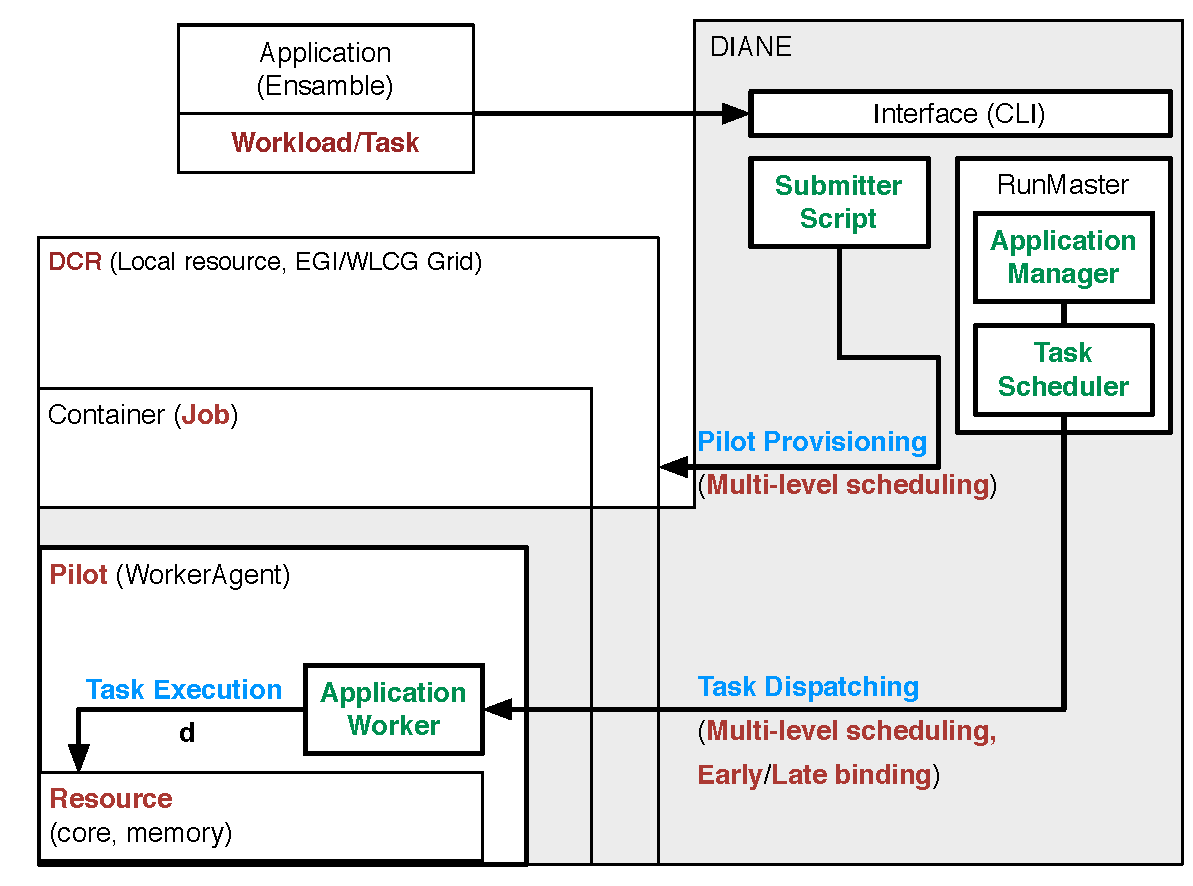
\includegraphics[width=.48\textwidth]{figures/diane_comparison.pdf}
    \caption{Diagrammatic representation of DIANE components,
    functionalities, and core vocabulary mapped on
    Figure~\ref{fig:core_vocabulary}.}
    \label{fig:diane_comparison}
\end{figure}

% Execution model.
The execution model of DAINE can be summarized in four
steps~\cite{moscicki2011understanding}: 1. the user submits one or more jobs to
DCR by means of SubmitScript(s) to bootstrap one or more WorkerAgent; 2. When
ready, the WorkAgent(s) reports back to the ApplicationManager; 3. tasks are
scheduled by the TaskScheduler on the available WorkerAgent(s); 4. after
execution, WorkerAgents send the output of the computation back to the
ApplicationManager.

%% 5 core properties

% Pilot Resources
The pilots used by DIANE bind compute resources on the target DCRs.
ApplicationAgents are executed by the DCR middleware as jobs with mostly one
core but possibly more. DIANE offers also a data service with a dedicated API
and CLI that allows for staging files in and out of ApplicationAgents. This
service represents an abstraction of the data resources and capabilities offered
by the DCR and it is designed to handle data only in the form of files stored
into a file system. Network resources are assumed to be available and no
abstractions are offered.

% Pilot Deployment
DIANE leaves the user free to develop deployment mechanisms tailored to specific
resources. The RunMaster service assumes to have pilots available to schedule
the tasks of the workload. Deployment mechanisms can range from direct manual
execution of jobs on remote resources to deployment scripts or full-fledged
factory systems to support the sustained provisioning of pilots over extended
periods of time.

A computational task-management tool called
GANGA~\cite{moscicki2009ganga,ganga_url} is available to support the development
of SubmitterScripts. GANGA offers a unified interface for job submission to DCRs
with Globus, Condor, UNICORE, or gLite middleware. The main goal of GANGA is to
facilitate the submission of WorkerAgents (i.e. pilots) to diverse DCRs by means
of a uniform interface and abstraction.

% Workload Semantics
DIANE has been designed to execute workloads that can be partitioned into
ensembles of parametric tasks on multiple ApplicationAgents. Each task can
consist of an executable invocation but also of a set of instructions, OpenMP
threads, or MPI processes~\ref{moscicki2011b}. Relations among tasks and group
of tasks can be specified before or during runtime enabling DIANE to execute
articulated workflows. Plugins have been written to manage
DAGs~\cite{grzeslo2009} and data-oriented workflows~\cite{glatard2008}.

% workload binding
DIANE is primarily designed for HTC/Grid environments and to execute pilots with
a single core. Nonetheless, the notion of ``capacity'' is exposed to the user to
allow for the specification of pilots with multiple cores. Although the workload
binding is controllable by the user-programmable TaskScheduler, the general
architecture is consistent with a pull model. The pull model naturally
implements the late-binding paradigm where every ApplicationAgent pulls a new
task once it is available and has free resources.

% ------------------------------------------------------------------------------
% Glidein
%
\subsubsection{HTCondor Glidein and GlideinWMS}
\label{sec:glidein}

% Who did it and for what scientific domains.
The HTCondor Glidein system has been designed as part of the software ecosystem
of HTCondor. The HTCondor Glidein system implements pilots within regular Condor
pools.  Developed by by the Center for High Throughput Computing at the
University of Wisconsin-Madison (UW-Madison), HTCondor Glidein's main goal was
originally to include DCRs exposing grid middleware, into Condor
pools~\cite{glidein_manual_url}.
\jhanote{I'm not sure the meaning of the previous sentence is clear: does it
mean (a) DCRs that expose grid middleware into a pool, (b) although we don't
define/use federate, does ``include'' actually refer to federate?} \mtnote{I
would not think so. A condor pool is a list of DCRs with a set of properties for
each item of the list. I added a comma, better? That sentence needs to convey
the following: there is a condor pool, there are DCRs with a grid middleware
(i.e. Globus), these DCRs need to be added to the condor pool; The HTCondor
Glidein system does that.}

 \mtnote{Find out metrics on usage and target scientific communities}

% Architecture.
The HTCondor components relevant to the Glidein system are: a set of Schedd and
Startd daemons, a Collector, and a Negotiator~\cite{glidein_presentation_url}.
Schedd is a queuing system that holds workload tasks and Startd handles the DCR
resources. The Collector holds references to all the active Schedd/Startd
daemons, and the Negotiator matches tasks queued in a Schedd to resources
handled by a Startd.

HTCondor Glidein has been complemented by
GlideinWMS~\cite{sfiligoi2008glideinwms}, a Glidein-based workload management
system that automates deployment and management of glideins on multiple types of
DCR middleware. GlideinWMS builds upon the HTCondor Glidein system by adding the
following components: a set of Glidein Factory daemons, a set of VO Frontend
daemons, and a Collector dedicated to the
WMS~\cite{glideinwms_url,glideinwms_manual_url}. Glidein Factories submits tasks
to the DCRs middleware, each VO Frontend matches the tasks on one or more Schedd
to the resource attributes advertised by a specific Glidein Factory, and the WMS
Collector holds references to all the active Glidein Factories and VO Frontend
daemons.

% \jhanote{I have the original text commented below. I reorganized a bit so as
%   to help the flow better. Also, we were introducing too many concepts in the
%   first couple of paragraphs which was getting difficult to parse. HTCondor,
%   glidein, glideninWMS, etc. This is a bit more gradual in terms of the rate
%   at which concepts are introduced}

% Why it is a pilot system.
Figure~\ref{fig:glidein_comparison} shows the mapping of the HTCondor Glidein
Service and GlideinWMS elements to the components and functionalities of a pilot
system as described in~\S\ref{sec:understanding}. The set of VO Frontends and
Glidein Factories alongside the WMS collector implement a Pilot Manager and its
pilot provisioning functionality. The set of Schedds, the Collector, and the
Negotiator implement a Workload Manager and its task dispatching functionality.
The Startd daemon implements a Task Manager alongside its task execution
functionality. A glidein is a job submitted to a DCR middleware that, once
instantiated, configures and executes a Startd daemon. As such, a glidein is a
pilot.

\begin{figure}[t]
    \centering
        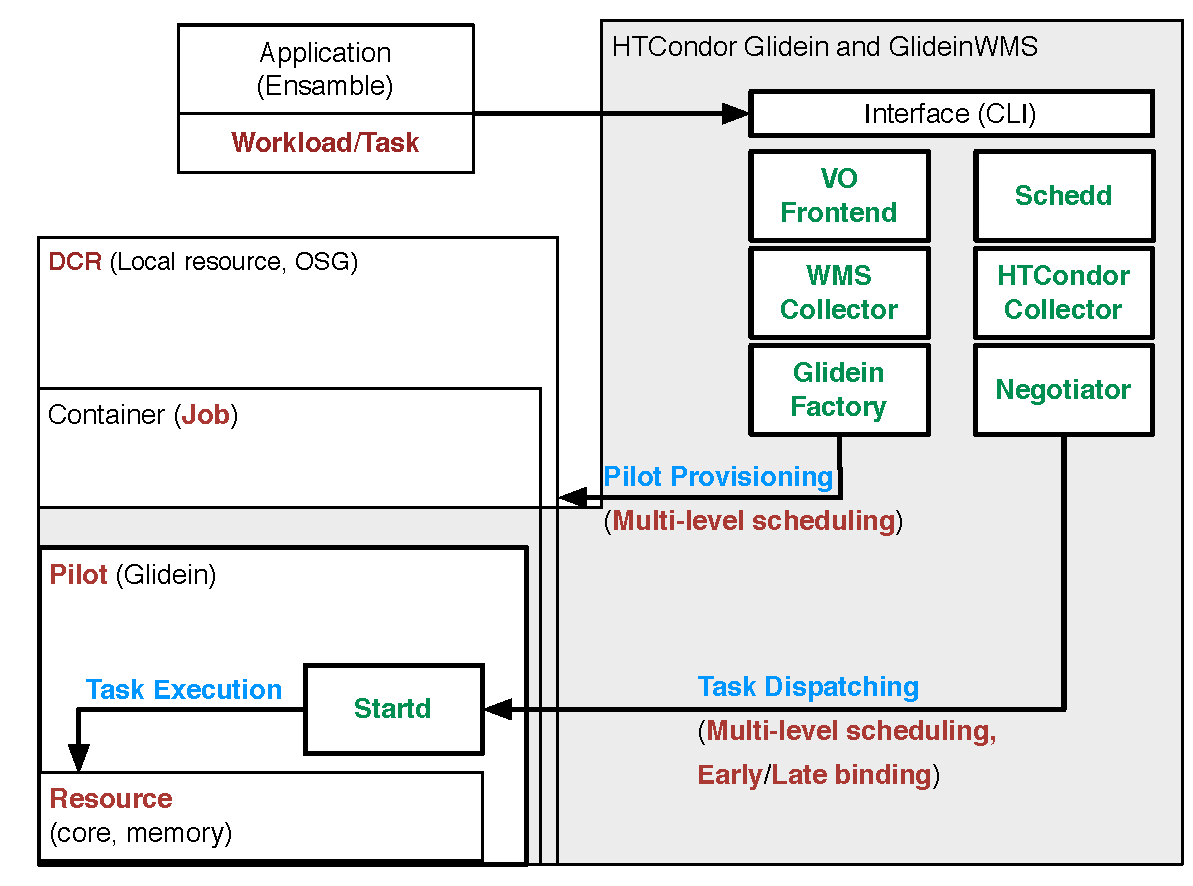
\includegraphics[width=.48\textwidth]{figures/glidein_comparison.pdf}
        \caption{Diagrammatic representation of Glidein components,
          functionalities, and core vocabulary mapped on
          Figure~\ref{fig:core_vocabulary}. \jhanote{minor typo: gladein factory
            needs to be replaced with glidein factory, and stard with startd}\mtnote{Done.}}
    \label{fig:glidein_comparison}
\end{figure}

% Execution model.
The execution model of the HTCondor Glidein system can be summarized in eight
steps: 1. the user submits a glidein (i.e. a job) to a DCR batch scheduler; 2.
once executed, this glidein bootstraps a Startd daemon; 3. the Startd daemon
advertises itself with the Collector; 4. the user submits the tasks of the
workload to the Schedd daemon; 5. the Schedd advertises these tasks to the
Collector; 6. the Negotiator matches the requirements of the tasks to the
properties of one of the available Startd daemon (i.e. a glidein); 7. the
Negotiator communicates the match to the Schedd; 8. the schedd submits the tasks
to the Startd daemon indicated by the Negotiator.

GlideinWMS extends the execution model of the HTCondor Glidein system by
automating the glideins provision. The user does not have to submit glidein
directly but only tasks to Schedd. From there: 1. every Schedd advertises its
tasks with the VO Frontend; 2. the VO Frontend matches the tasks' requirements
to the resource properties advertised by the WMS Connector; 3. the VO Frontend
places requests for glideins instantiation to the WMS Collector; 4. the WMS
Collector contacts the appropriate Glidein Factory to execute the requested
glideins; 5. the requested glideins become active on the DCRs; and 6. the
glideins advertise their availability to the (HTCondor) Collector. From there
on the execution model is the same as described for the HTCondor Glidein
Service.

%% 5 core properties.

% Pilot Resources.
The resources managed by a single glidein (i.e. pilot) are limited to compute
resources. Glideins may bind one or more cores, depending on the target DCRs.
For example, heterogeneous HTCondor pools with resources for desktops,
workstations, small campus clusters, and some larger clusters will run mostly
single core glideins. More specialized pools that hold, for example, only DCRs
with HTC/grid/cloud middleware may instantiate glideins with a larger number of
cores. Both HTCondor Glidein and GlideinWMS provide abstractions for file
staging but no pilot abstraction is offered for data or network resources.

% Pilot Deployment.
The process of pilot deployment is the main difference between HTCondor Glidein
and GlideinWMS. While the HTCondor Glidein system requires users to submit the
pilots to the DCRs, GlideinWMS automates and optimizes pilot provisioning.
GlideinWMS minimizes resource utilization and maximizes the throughput of task
execution by continuously instantiating glideins until the queue of the
available Schedds are emptied. Once all the tasks have been executed, the
remaining glideins are terminated.\jhanote{not sure what ``minimizes the amount
of resource utilization'' means?} \mtnote{That uses as little resources as
possible to execute the given tasks. Better?}

% Workload Semantics.
HTCondor Glidein and GlideWMS expose the interfaces of HTCondor to the
application layer and no theoretical limitations are posed on the type and
complexity of the workloads that can be executed. For example, DAGman (Directed
Acyclic Graph Manager)~\jhanote{reference needed}\mtnote{I still have to add all
the references.} has been designed to execute workflows by submitting tasks to
Schedds, and a \MW tool is available to design applications with a \MW execution
pattern. \jhanote{the second ``d'' in schedd is the daemon..} \mtnote{The word
is capitalized so the `d' is part of the name of the component, not an
abbreviation or a letter of an acronym.}
\jhanote{what is the name of the master-worker tool?} \mtnote{It is called like
that: `\MW tool'.}

In practice, as HTCondor has been originally designed for resource scavenging
and opportunistic computing, single or low-core, independent tasks are more
commonly executed than multi-core, possibly parallel tasks. For example, this is
the case for OSG, the largest HTCondor and GlideinWMS deployment. Nonetheless,
it should be noted that specific projects may use dedicated installation and
resources to execute tasks with larger core requirements both for distributed
and parallel applications, including MPI applications. \jhanote{I'm not sure I
understand the rationale of the last sentence?} \mtnote{Get a cluster with
multi-core compute nodes and fast interconnect (and possibly add a bunch of
separate machines/VMs); install all the HTCondor stack + the GlideinWMS and the
headnode (and possibly on the separate machines); now you can run your
distribute, parallel, MPI applications on that cluster via glideins. As far as I
understand, there is no intrinsic limitation built within HTCondor or GlideinWMS
to the execution of distributed, parallel, and MPI applications. Executing only
distributed applications, mostly with single-core tasks is a consequence of the
type of resources that are added to a Condor pool.}

% workload binding.
Both HTCondor Glidein and GlideWMS rely on one or more HTCondor Collectors to
match task requirements and resource properties. This matching can be evaluated
right before the execution of the task. \jhanote{is this match-maker the
ClassAds, or is there another level of match-makeing for the glideins?} \mtnote{
There is lack of documentation but I assume the Collector is the component where
the matchmaking function is implemented. ClassAds should be the name given to
the entries published by the Glidein Factories within the WMS collector (in the
case of GlideinWMS but it should be the same with the old HTCondor Glidein)} As
such, both pilot systems allow for late binding. Early binding is not available.

% ------------------------------------------------------------------------------
% PANDA
%
\subsubsection{PANDA}
\label{sec:panda}


\mtnote{NOTE: references needs to be added to the whole subsection.}

% Who did it and for what scientific domains.
\panda (Production and Distributed Analysis)~\cite{1742-6596-331-7-072069} was
developed to provide a multi-user workload management system (WMS) for
ATLAS~\cite{aad2008atlas}. ATLAS is a particle detector at the Large Hadron
Collider (LHC) at CERN that requires a WMS to handle large numbers of tasks for
their data-driven processing workloads. In addition to the logistics of handling
large-scale task execution, ATLAS also needs integrated monitoring for analysis
of system state and a high degree of automation to reduce user and
administrative intervention.

\panda has been initially deployed as an HTC-oriented, multi-user WMS system for
ATLAS, consisting of ~100 heterogeneous computing sites~\cite{maeno_pd2p:_2012}.
Recent improvements to \panda have extended the range of deployment scenarios to
HPC and Cloud-based DCRs making \panda a general-purpose \pilot
system~\cite{nilsson2012recent}.

% Architecture.
\panda architecture consists of a Grid Scheduler and a \panda Server. The Grid
Scheduler is implemented by a component called `AutoPilot' that submits jobs to
diverse DCRs. The \panda server is implemented by four main components: a Task
Buffer, a Broker, a Job Dispatcher, and a Data Service. The Task Buffer collects
all the submitted tasks into a global queue and the Broker prioritizes and binds
those tasks to DCRs on the basis of multiple criteria. The Data Service stages
the tasks' input file(s) to the DCR to which the tasks have been bound using the
data transfer technologies exposed by the DCR middleware (e.g. uberftp, gridftp,
or lcg-cp). The Job Dispatcher delivers the tasks to the RunJob(s) running on
the bound DCR.

% Why it is a pilot system.
Figure~\ref{fig:panda_comparison} shows how PANDA implements the components and
functionalities of a pilot system as described in~\S\ref{sec:understanding}: the
Grid Scheduler is a Workload Manager implementing Pilot Provision while the
\panda Server is a Task Manager implementing Task Dispatching. The jobs
submitted by the Grid Scheduler are called `Pilots' and act as pilots once
instantiated on the DCR by contacting the Job Dispatcher component to request
for tasks to execute.

\begin{figure}[t]
    \centering
        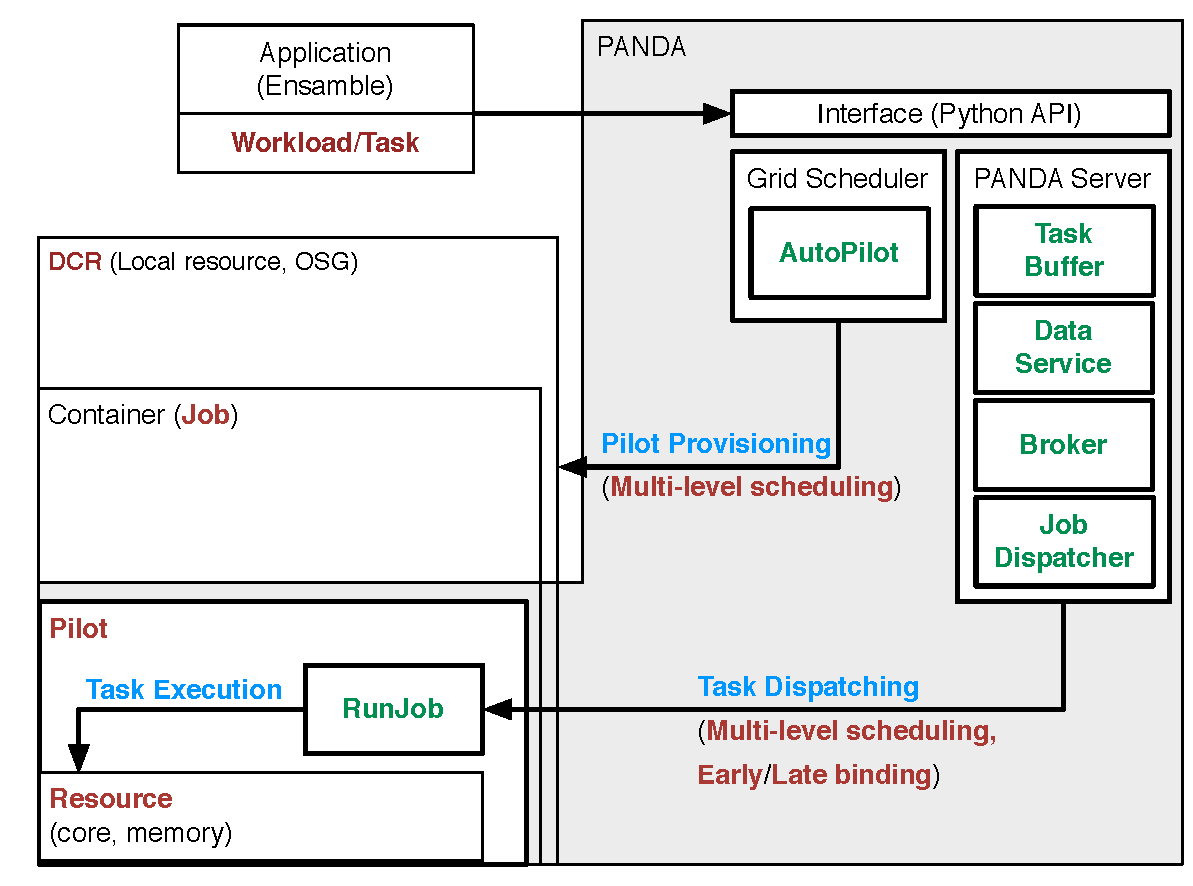
\includegraphics[width=.48\textwidth]{figures/panda_comparison.pdf}
    \caption{Diagrammatic representation of PANDA components, functionalities,
    and core vocabulary mapped on Figure~\ref{fig:core_vocabulary}.}
    \label{fig:panda_comparison}
\end{figure}

% Execution model.
The execution model of PANDA can be summarized in seven steps: 1. the user
submits tasks to the \panda server; 2. the tasks are queued within the Task
Buffer; 3. the tasks requirements are evaluated by the Broker and bound to a
DCR; 4. the tasks' input files are staged to the bound DCR by the Data Service;
5. the required pilot(s) are submitted as jobs to the target DCR; 6. the
submitted pilot(s) becomes available and reports back to the Job Dispatcher;
7. tasks are dispatched to the available pilots for execution.

%% 5 core properties.

% Pilot Resources.
\panda pilots expose computational resources. Pilots are designed to expose
mainly a single core but extensions have been developed to instantiate pilots
with multiple cores. The Data Service of \panda allows to integrate and automate
data staging within the task execution process but no pilot-based data
abstractions are offered. Network resources are assumed to be available but no
network-specific abstractions are made available.

% Pilot Deployment.
The AutoPilot component of \panda's Grid Scheduler has been designed to use
multiple methods to submit pilots to DCRs. The \panda installations of the US
ATLAS infrastructure uses the HTCondor-G system to submit pilots to the US
production sites. Other schedulers enable AutoPilot to submit to local and
remote batch systems or to the GlideinWMS frontend. Submissions via the
canonical tools offered by HTCondor have also been used to submit tasks to cloud
resources via
\panda.

% Workload Semantics.
\panda was initially designed to serve specifically the ATLAS use case and, as
such, to execute mostly single-core tasks with input and output files. Since its
initial design, the ATLAS analysis and simulation tools have started to
investigate multi-core task execution with AthenaMP~\cite{crooks2012} and \panda
has been evolving towards a general purpose workload manager. As a consequence,
\panda is starting to offer experimental support for multi-core pilots and tasks
with or without data dependences. \panda also now supports applications from a
variety of science domains.\cite{x,y}.

% workload binding.
\panda offers late binding but not early binding capabilities. Workload jobs are
assigned to activated and validated pilots by the \panda server based on
brokerage criteria like data locality and resource characteristics.

% ------------------------------------------------------------------------------
% RADICAL PILOT
%
\subsubsection{RADICAL-Pilot}
\label{sec:radical_pilot}

% Who did it and for what scientific domains.
The authors of this paper have been engaged in theoretical and practical aspects
of \pilot systems for the past several years. In addition to formulating the P*
Model~\cite{luckow2012} which by most accounts is the first complete conceptual
model of a pilot system, the RADICAL group is responsible for the development
and maintenance of RADICAL-Pilot\cite{rp-paper2015,rp_url}. RADICAL-Pilot is the
group's long-term effort for creating a production level \pilot system. The
effort is built upon the experience gained from developing and deploying
BigJob~\cite{luckow2010}, and and integrating it with many applications on
different DCRs~\cite{x,y,z}.

% Architecture.
RADICAL-Pilot consists of three main components: a Pilot Manager, a Compute Unit
(CU) Manager, and a set of Agents. The Pilot Manager describes pilots and then
submit them to DCR, while the CU manager describes tasks (i.e. CU) and schedules
them to one or more pilots. Agents are instantiated on DCRs and execute the CUs
pushed by the CU manager.

% Why it is a pilot system.
RADICAL-Pilot has been specifically designed to be a \pilot system and, as seen
for example with DIANE, it closely resembles the description offered
in~\S\ref{sec:understanding} (see Figure~\ref{fig:panda_comparison}). The Pilot
Manager and the Workload Manager are implemented by the CU Manager. The Agent is
deployed on the DCR to expose its resources and execute the tasks pushed by the
CU Manager. As such, the Agent is a pilot.

\begin{figure}[t]
    \centering
        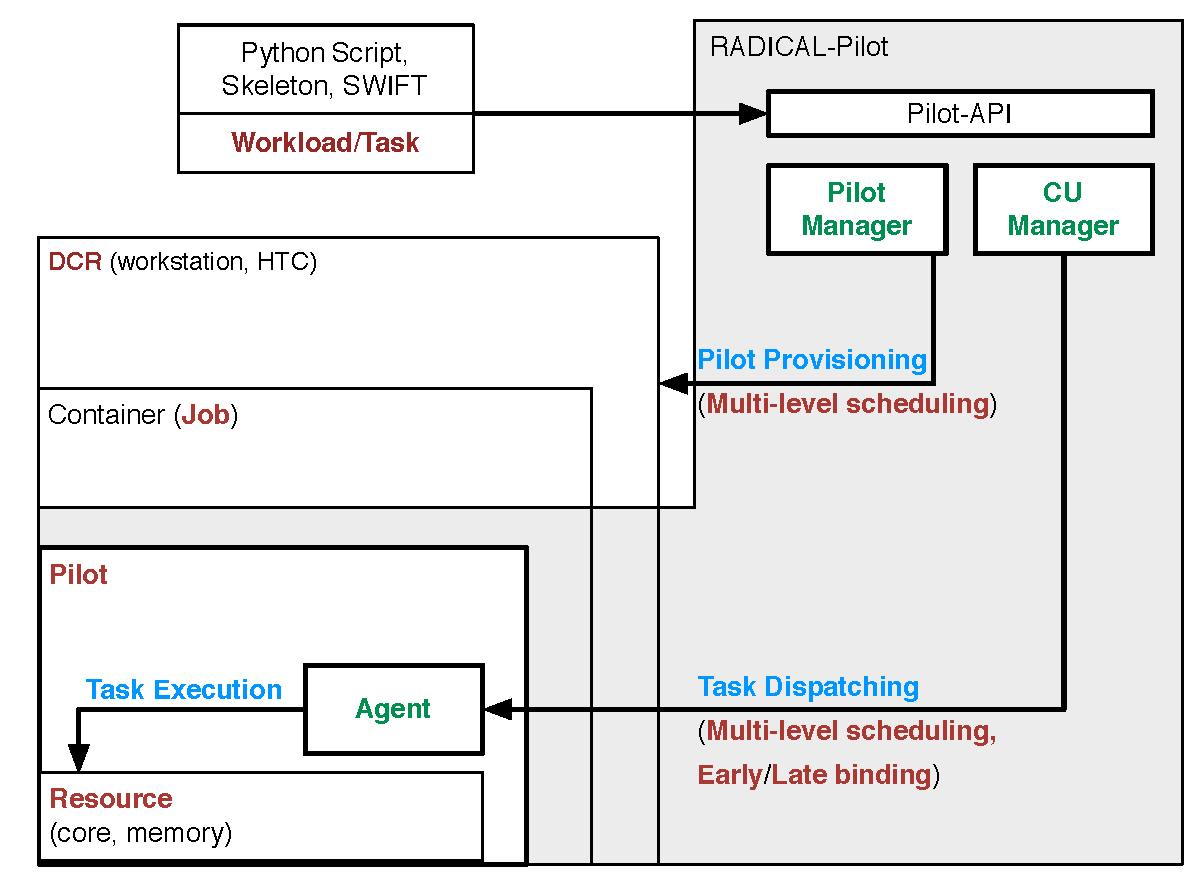
\includegraphics[width=.48\textwidth]{figures/radicalp_comparison.pdf}
    \caption{Diagrammatic representation of RADICAL Pilot components,
    functionalities, and core vocabulary mapped on
    Figure~\ref{fig:core_vocabulary}.}
    \label{fig:rp_comparison}
\end{figure}

% Execution model.
RADICAL-pilot is implemented as a python module that a user can use to design
and code a distributed application. The execution model of RADICAL-Pilot is as
follows: 1. the user describes tasks as a set of CUs with or without data and
DCR dependences; 2. the user also describes one or more pilots choosing the
DCR(s) where they should be submitted to; 3. The Pilot Manager submits each
pilot that has been described to the indicated DCR; 4. The CU Manager schedules
each CU either to the pilot indicated in the CU description or on the first
pilot with free and available resources; 5. when required, the CU Manager stages
also the CU's input file(s) to the target DCR; and 6. the Agent executes the CU.
Eventually, if needed the output files of the CU can be staged to a user-defined
destination. \jhanote{need to add reference to the figure..} \mtnote{Done.}

%% 5 core properties.

% Pilot Resources.
The Agent component of RADICAL-Pilot offers abstractions for both compute and
data resources. Every Agent can expose between one and all the cores of the
compute node where it is executed, and it can also expose a data handle that
abstracts away specific storage properties and capabilities~\cite{luckow2010}.
In this way, the CUs running on a Agent can benefit from unified interfaces both
to core and data resources. Network resources are assumed to be available and no
pilot abstraction is offered for their abstraction.

% Pilot Deployment.
The Pilot Manager deploys the Agents of RADICAL-Pilot by means of the
SAGA-python API~\cite{sagax}. SAGA provides access to diverse DCR middleware via
an unified and coherent API, and thus RADICAL-Pilot can submit pilots to all the
resources exposed by XSEDE, by the OSG HTCondor pools, and many ``leadership''
class systems like those managed by NERSC~\cite{nersc_url},
OLCF~\cite{olcf_url}, or NCSA~\cite{ncsa_url}. Adding support for a new DCR is
relatively simple, as proven for example with the ongoing inclusion of a
LRZ~\cite{lrz_url} petascale system and IaaS DCRs. \jhanote{not sure we want to
mention hopper, titan and bluewaters or supermuc as they are likely to become
``dated'' soon. thoughts?} \mtnote{Better?}



% Workload Semantics.
RADICAL-Pilot can execute tasks with varying degree of coupling and
communication requirements. Tasks can be completely independent, single or
multi-threaded; they may be loosely coupled requiring input and output files
dependences, or they might be tightly coupled requiring low-latency runtime
communication. As such, RADICAL-Pilot supports MPI applications, workflows, and
diverse execution patterns such as simulation/analysis, Replica Exchange
simulations, or pipelines~\cite{emdtoolkit_url}.

% workload binding.
CU descriptions may or may not contain a reference to the pilot to which the
user wants to bind the CU. When a reference is present, the scheduler of the CU
Manager waits for a slot to be available on the indicated pilot. When a target
pilot is not specified and more pilots are available, the CU Manager schedules
the CU on the first pilot available. As such, RADICAL-Pilot supports both early
and late binding, depending on the use case and the user specifications.

% -----------------------------------------------------------------------------
% 4.3
%
\subsection{Implementation Differences and Overall observations}
\label{sec:context}

\mtnote{Some of the auxiliary properties are missing from the following
analysis. More discussion about whether we have something relevant to say about
them is needed.}

% \paragraph*{HTC and HPC}

The analysis offered in the previous subsection shows how diverse \pilot system
implementations conform to the set of components and functionalities defined
in~\S\ref{sec:understanding}. These sets are therefore minimal but also
necessary, as the implementation descriptions showed that \pilot deployment,
task submission, and task execution functionalities have to be implemented in
order to enable the execution of task-based workloads by means of multi-level
scheduling.

The analysis of DIANE, HTCondor Glidein, GlideinWMS, PANDA, and RADICAL-Pilot
highlighted also implementation differences, especially concerning the auxiliary
properties of these \pilot systems. For example, based on the description of the
auxiliary properties offered in~\S\ref{sec:auxprops}, the described \pilot
systems showed not only evident variations in their architectures and data
management capabilities, but also in their DCR interaction model, their
interfaces, and interoperability. Here these differences are described widening
the scope of the analysis also to other relevant auxiliary properties.

The goal is not only to highlight the differences among \pilot systems but also
to show their implementation challenges. In this way, the following analysis can
contribute clarity and useful indications to the evolution process the \pilot
systems implementations are undergoing. Furthermore, clarifying the differences
among \pilot systems implementations could also offer relevant indications on
how and when a specific implementation should be adopted.

% Architecture (DONE in previous subsection)

% Coordination and communication

% Interoperability
The \pilot systems described in the previous subsection offer a varying degree
of interoperability across diverse DCRs. For example, DIANE and PANDA were
initially designed to support mostly the Grid-based DCRs used by the LHC
experiments, while HTCondor Glidein and GlideinWMS to execute tasks on the
Condor-based DCRs. With the progressive development of both the \pilot systems
and the DCR middleware, more types of DCR are being supported, highlighting the
relevance of task execution localization.

The notion of task as defined in~\S\ref{sec:understanding} and then utilized
in~\S\ref{sec:implementations} shapes both the design and implementation of
\pilot systems. Design-wise, adding a wrapper to the executables of a
distributed or parallel application means creating a well-defined space for
their localization. This may involve not only the specification of program
switches, data locations, or library dependences but also loading modules,
downloading supporting code, or on-the-fly compilations and execution of
supporting applications. Implementation-wise, localization requires tight
coupling with the target DCR, its capabilities, policies, and specific
configurations.

The implementation of the localization process becomes more challenging in the
presence of heterogeneous DCRs. The same executable may require different
localization procedures depending on where it will be executed. More
importantly, different types of localizations may or may not be available or
allowed on all the target DCRs. This imposes decision capabilities on the task
scheduler and the development of a robust interoperability layer between the
\pilot system and heterogeneous target DCRs.

% Resource Overlay

Interoperability across DCRs is a necessary preconditions to utilize multiple
pilots across diverse DCRs. In a multi-pilot, multi-DCR scenario, the relations
among resources and task requirements increase in number and complexity. Data
not only needs to be replicated and made available across different locations
but the applications and protocols used to move data may change across target
DCRs. DCR with specialized data capabilities may have to be prioritized
depending on the data requirements of the tasks or, analogously, DCR supporting
specific types of compute resources may have to be chosen when, for example,
applications require GPU compute cards.

In this context, \pilot systems need to support higher level abstractions such
as resource affinity~\cite{luckow2014pilot,neumeyer2010s4} or multidimensional
scheduling~\cite{zhu2008multi}. The correlation among data, compute, and network
resources needs to be assessed for every execution and carefully leveraged to
optimize not only time to completion but also resource utilization. These
optimizations may be the determining factor to enable the execution of
applications with stringent data, compute, or networking requirements.

Given these requirements, it is not surprising that GlideinWMS and PANDA have
began to support multi-pilot, multi-DCRs executions. These \pilot systems
implement articulated workload management components with well-isolated
scheduling elements and robust communication and coordination infrastructures.
Without such an architecture, a robust implementation of the higher-level
capabilities required by multi-pilot, multi-DCR task executions would be very
challenging.

% Files and Data

The relevance of both compute and data resources is shown by the implementation
of dedicated capabilities in all the \pilot systems described in the previous
subsection. Along the use of pilots to expose compute resources, \pilot systems
utilize dedicated subsystems to manage data staging. Data staging is coordinated
with task executions and implemented by utilizing the file-transfer capabilities
exposed by the DCR middleware.

The data abstraction utilized by all the reviewed \pilot systems is
file-centric. Data are expected to be aggregated into input/output files that
need to be transferred between workstations, data repository, or DCR filesystems
across the networking infrastructure. This assumptions may be limiting,
especially when considering data-intensive applications.

Support for diverse technologies and higher-level abstractions is likely to
become a requirement for the development of general purpose \pilot systems. For
example, transparent support for distributed filesystems like
HDFS~\cite{borthakur2008}, opportunistic creations of data clusters like those
utilized by YARN~\cite{vavilapalli2013}, transparent integration of databases or
storage services are likely to play a relevant role in the efficient execution
of data-oriented, distributed
applications~\cite{rey2015open,sboner2015primer,zhang2010}.

% Robustness
% Performance and Scalability
% Development Model

% DCR Interaction

The \pilot systems described in the previous subsection present differences also
in the two auxiliary properties DCR Interaction and Interface. GlideWMS, PANDA,
and RADICAL-Pilot support diverse DCR middleware including typical HPC, Grid,
and Cloud batch systems. As seen in~\S\ref{fig:core_vocabulary}, this
flexibility is possible due to the generality of the notion of resource
placeholder and its independence from the specificities of the target
infrastructures and their middleware. Placeholders abstract the notions of
resources, scheduling, and task execution, creating a well-defined and isolated
logical space for the management of task execution. It remains to be understood
in what conditions and for what type of application each implementation of a
placeholder is more appropriate.

% Interfaces

Each \pilot system described in the previous subsection exposes a different
interface. DIANE, HTCondor Glidein, GlideinWMS, and PANDA offer command line
tools tailored to specific use cases, applications, and DCRs. RADICAL-Pilot
exposes instead an API but both the DIANE and PANDA command line tools are built
on API that users may directly access and use to develop distributed
applications. This degree of heterogeneity can be justified with special-purpose
\pilot systems but it may lead to fragmentation and duplication of effort with
general-purpose systems.

The current state of the workflow systems~\cite{taylor2014} is a paradigmatic
example of this risk. Many workflow systems have been implemented with
significant duplication of effort and limited means for extensibility and
interoperability. One important contributing factor to these limitations is the
lack of suitable, open, and possibly standard-based interfaces for the resource
layer. Most workflow engines are developed with proprietary solutions to access
the resource layer; solutions that cannot be shared with other engines and that
often serve specific requirements, use cases, and infrastructures.

Open APIs like the one specified in~\cite{luckow2012b} and implemented by
RADICAL-Pilot offer the missing layer on which workflow and, more generally,
distributed applications could be built upon. As with the resource layer, \pilot
systems offers a well-defined and well-isolated layer between applications and
resources. This fosters extensibility, interoperability, and modularity by
separating the application description and logic from the management of its
execution, and from the provisioning and aggregation of resources. In turn, this
avoids the need to develop special-purpose, vertical, and end-to-end
applications, the main source of duplication and fragmentation in the current
distributed application and tooling landscape.

% Security and multitenancy

Finally, DIANE, HTCondor Glidein, GlideinWMS, PANDA, and RADICAL-Pilot implement
different types of authentication, authorization, and accounting processes
(AAA). Nonetheless, the AAA requirements specific to \pilot system
implementations can be limited to: (i) the single or multitenancy of the
instantiated pilots; and (ii) the credentials used to submit pilots to the DCRs.

The AAA required by the user to access her own pilots varies depending on the
pilot's tenancy. With single tenancy, the pilot can be accessed only by the user
that submitted it. As such, AAA can be based on inherited privileges. With
multitenancy, the \pilot system has to evaluate whether a user requesting access
to a pilot is part of the group of allowed users. Among the described \pilot
systems, HTCondor Glidein and GlideinWMS are the only two implementing pilot
multitenancy and using advanced abstractions like VOs and federated certificate
authorities~\cite{horwitz2002}.

The credential used for pilot deployment depends on the target DCR. The AAA
requirements of DCRs are a diverse and often inconsistent array of mechanisms
and policies. \pilot systems are gregarious in the face of such a diversity as
they only need to present the credentials provided by the application layer (or
directly by the user) to the DCR. As such, the requirements for AAA
implementation within \pilot systems are minimal.


% ------------------------------------------------------------------------------
% Section 4's concluding remarks
%
% \subsection{Overall observations}

% The descriptions and analyses offered in Subsections~\ref{sec:implementations}
% and~\ref{sec:context} shows the relevance of at least three characteristics of
% \pilot system implementations: interoperability layers, automation of pilot
% provision, and type of implemented architecture.

% The interoperability layer enables the implementations of a Pilot Manager to
% submit pilots to diverse DCRs. As such general-purpose \pilot systems depend
% upon this layer and the capabilities that exposes.

% \begin{itemize}

% \item Importance on interoperability layers/libraries over DCRs' middleware
% (e.g. GANGA, SAGA)

% \item Importance of automating pilot provisioning as opposed to leave the task
% tot he user to develop deployment scripts.

% \item Remark consistency of implementation architectures with the one given in
% 3.

% \item Use three dimensions (D (dependency) C (coupling) and H (heterogeneity)
%   ) (D I H) to analyze types of workloads. \jhanote{Is ``I'' independent?.
%   Also we might want to add ``N'' -- cardinality, which captures the number of
%   tasks in the workload.}

% \item Accessory properties is what determine whether potential capabilities
% can be translate into practical executions. E.g. while Condor allows for
% execution of parallel applications, in practice the requirements in terms of
% software and configuration imposed on the DCR make very difficult or
% undesirable to expose resources from DCR with HTC-size compute nodes.

% \item Analyze different implementation methods underlying the differences in
% usability and requirements between frameworks and full-fledged applications.
% ``Some of systems we have discussed, like DIRAC, X, are inherently service
% oriented, or exposed as a service. On the other side of the spectrum, systems
% like DIANE and RADICAL-Pilot take the form of a library or a framework. From a
% formal standpoint, services can be abstracted by a library and a library can
% be abstracted by a service, so the main distinction between these
% architectures if the default form they come in and how they are meant to be
% deployed.''

% \item Other Pilot Systems: We have discussed only a limited number of
% \pilots systems that exist; this is purely a reflection of the limitations of
% space. We eschewed coverage in favour of favour of completeness of a the few
% \pilot systems. \jhanote{As discussed we'll have a closing paragraph or two,
%   about all the pilot systems that we don't discuss}


% \end{itemize}


% -----------------------------------------------------------------------------
% SECTION 5
% -----------------------------------------------------------------------------
%
\section{Discussion and Conclusion}
\label{sec:discussion}

\jhanote{General note: (i) needs major reduction, (ii) needs 4.2 to be complete
  before this section will get desired/needed punch, (iii) needs elaboration of
  P*.}


% \jhanote{the structure of section 5 is: (i) revisit the myths. (ii)
% state clearly how section 3 and 4 help us define what a pilot is,
% the necessary and sufficient conditions (if possible), discuss the
% classifiers and apply/discuss them to the set of pilot systems here.
% (iii) then we go on to say motivate P*/pilot for data, (iv) discuss
% implications for WF systems and conclude with a summary for
% tools/sustainability/etc. At some point, we discuss how/why pilots
% are more than just pilots, eg can be RM layer for middleware,
% runtime framework etc}\mtnote{I have organized the following items on
% the lines you have traced, with some changes in the order and number
% of the items.}

% \mtnote{In Section 3 we use pilotjob. We will have to move to \pilot or decide
% to use the less correct pilotjob here too.}\mtnote{Following discussion, we
% decided to use \pilot. Section 3 has been updated, the other Sections will
% have to follow.}

Section~\ref{sec:understanding} offered a description of the minimal
capabilities and properties of a \pilot system alongside a vocabulary defining
`\pilot' and its cognate concepts. Section~\ref{sec:analysis} offered a
classification of the core and auxiliary properties of \pilot system
implementations, and the analysis of an exemplar set of \pilot system
implementations. Considered altogether, these contributions outline the
characteristics and properties of a paradigm for the execution of tasks on
distributed resources by means of resource placeholders. This is here referred
to as `\pilot paradigm'.

In this section, the properties of the \pilot paradigm are critically assessed.
The goal is to show the generality of this paradigm and how \pilot systems go
beyond the implementation of a special purpose solutions to speed up the
execution of a certain type of workload.
% Once the breadth of the \pilot paradigm has been understood, it is
% contextualized by describing its relation with relevant domains such as
% middleware, applications, security, and the enterprise.  Finally,
The section closes with a look into the future of \pilot systems moving from the
current state of the art and discussing the sociotechnical and engineering
challenges that are being faced both by developers and target users.

\jhanote{A suggestion for the organization of S5: Establish the generality of
  the concept in 5.1 via a discussion of ``internal'' core properties (task
  binding, execution...)  of the pilot (c.f. section 4.1). We move to 5.2 and
  discuss the generality with respect to ``external'' core properties. (I am not
  advocating for a formal bloat of terminology, but just as an internal
  organizational principle). 5.2 than speaks to the resource types, possibly
  workload semantics (might require shifting text around from 5.1) etc.. Also, I
  know in 5.2 we are trying to highlight that the paradigm remains the same, but
  the implementation of and application of the pilot paradigm differs.  It can
  speak to auxiliary properties such as AAA, but we know they are already fairly
  specific to an implementation, so we don't need to spend much real estate on
  specific auxiliary properties, but possibly generalize the challenges/reasons
  to the set of auxiliary properties.}

% \mtnote{Just an idea: Section 2 -- pilot abstraction; Section 3 --- pilot
% system; Section 4 --- Pilot implementation; Section 5 --- pilot paradigm.
% Abstraction: the conceptualization of pilot; system: the modeling of pilot
% conceptualization; implementation: the implementation of the model; paradigm:
% methods, tools, and procedures pertaining to/enabled by the use of pilots.
% What do you think? Happy to refine/change/abandon if you think it does not
% work.}

% -----------------------------------------------------------------------------
% 5.1
%
% The \pilot paradigm has been successfully integrated within workflow systems
% to support execution of workloads with articulated data and task dependencies.
% Furthermore, both single and multi-core tasks can be executed by many existing
% \pilot systems, with some of them also offering resource-specific MPI support.
% As such, depending on the type of the given workload, the \pilot paradigm can
% be implemented to optimize different metrics of task execution other than
% throughput. \

\subsection{The Pilot Paradigm}
\label{sec:paradigm}

% The \pilot paradigm is characterized and defined primarily by resource
% placeholding, multi-level scheduling, and late binding.

\pilot systems represents a category of software in itself.  Appreciating the
generality of the \pilot paradigm and the independence of its implementations
from other types of software, helps also to avoid a potential misunderstanding
that \pilots are not just an alternative implementation of a scheduler, of a
workload manager, of a batch system, or of any other special-purpose software
component. \jhanote{This paragraph could be transposed with the last paragraph
  in 5.1. Thoughts?}

%and how multi-level scheduling works. % \pilot systems do not
% circumvent the infrastructure middleware but abstract away some of its
% properties in order to optimize one or more user-defined (performance) metrics.
% Multi-level scheduling does not replace the infrastructure-level scheduler
% either. As clearly illustrated in~\S\ref{sec:understanding}, resource containers
% are still created on the target infrastructure by means of that infrastructure's
% capabilities and the second level of scheduling is completely contained within
% the boundaries of the resource container.
%\pilot systems are

The \pilot paradigm identifies a type of software system with both general and
unique characteristics. This paradigm is general because it does not strictly
depend on a single type of workload, a specific DCR, or a unique performance
metric. In principle, systems implementing the \pilot paradigm can execute
workloads composed by an arbitrary number of tasks with disparate requirements.
For example, as seen in~\S\ref{sec:analysis}, \pilot systems can execute
homogeneous or heterogeneous bags of independent or intercommunicating tasks
with arbitrary duration, data, or computation requirements.

The same generality applies to both the type of resource and of infrastructure
on which a \pilot system can execute workloads. As seen in
\S\ref{sec:understanding}, the \pilot paradigm demands resource placeholders but
does not specify the type of resource that the placeholder should expose.
% Nonetheless, most of the \pilot systems illustrated in \S\ref{sec:analysis}
% are designed to expose only compute resources, i.e. the cores of the compute
% nodes for which the pilot is a placeholder. Tasks executed on these \pilots
% may also use data or network resources but mostly as accessories to their
% execution on computational resources.  It is important to note that the focus
% on computational resources is not mandated by the \pilot paradigm.
In principle, pilots can be placeholders also and exclusively for data or
network resources, depending on the capabilities exposed by the middleware of
the target infrastructure.  For example, in Ref.~[pilot data] the concept of
\pilotdata was conceived to be fundamental to dynamic data placement and
scheduling as \pilot is to computational tasks.

\pilot systems already operate on multiple DCR. Originally devised for HTC
grid infrastructures, \pilot systems have been (re-)engineered to operate also
on HPC and Cloud infrastructures.
% It is important to note that many of the \pilot systems described in
% \S\ref{sec:analysis} have been adapted to work with different infrastructures
% without undergoing major re-architecturing. This is a further indication of the
% independence of the \pilot paradigm from infrastructural details, especially
% those concerning the type of container used to instantiate a placeholder.
Traditionally, \pilots have been thought of as a means to optimize the
throughput of single-core (or at least single-node), short-lived, uncoupled
tasks execution ~\cite{pordes2007,sfiligoi2009,juve2010}. The analysis presented
in~\S\ref{sec:analysis} showed that such a view is restrictive.  The \pilot
paradigm has been successfully integrated within workflow systems to support
execution of workloads with articulated data and single or multi-core task
dependencies.
% Furthermore, workload with multiple, possibly tightly-coupled components may use
% a \pilot system to provide not only a single entry point to the DCR scheduler,
% but also a dynamic resource allocation that grows or shrinks depending on the
% required resources.
As such, depending on the type of the given workload, the \pilot paradigm can be
implemented to optimize different metrics of task execution other than
throughput.

The generality of the \pilot paradigm may come as a surprise when considering
the requirement that has motivated most implementations, viz., leveraging
multi-level scheduling so as to increase the execution throughput of large
workloads made qof short running tasks.  For example, as seen
in~\S\ref{sec:analysis} \panda, Falkon, or DIRAC were initially developed as
single-point solutions, focusing on either a type of workload, a specific
infrastructure, or the optimization of a single performance metric.

Appreciating the properties of the \pilot paradigm becomes necessary once
requirements of infrastructure interoperability, support for multiple types of
workloads, or flexibility in the optimization of execution are introduced.
Satisfying those requirements requires abstracting the specificity of
middleware, infrastructure architectures, and application patterns. As shown in
this paper, this process of abstraction mandates the development of an
understanding of the \pilot paradigm.


% \mtnote{To be expanded with better/further examples of why we want to run MPI
% with pilots.}\jhanote{multiple possibly tight-coupled components use a pilot to
% provide (i) single point of entry to the scheduler for multiple components, (ii)
% growing/shrinking of resources needed for (interacting) components i.e., a
% different type of dynamic resource allocation} \jhanote{move to previous section
% where generality of workload is discussed} \mtnote{Done.}


% This specific system is used when abstracting one or more type of physical
% resources with well-defined spatial and time properties can lead to the
% optimization of one or more parameters of the workload execution. \jhanote{last
%   sentence can be deleted or needs attention to make straight and simple.}



% Optimizing the usage of the resource containers, for example by minimizing
% idling time, is an implementation issue, not an intrinsic limitation of the
% \pilot paradigm.  Shifting the control over tasks scheduling away from the
% infrastructure middleware does not imply that the end-user will become
% necessarily responsible for an efficient resource utilization. A \pilot system
% can be implemented as a middleware component, as seen with HTCondor and its role
% as an integral part of the infrastructure middleware stack on some DCIs.


\jhanote{We need 1-2 paragraphs describing the relationship of Section 3 to the
  P* model/paper. Else we are going to get dinged by reviewer or cause confusion
  to the reader. Where this paragraph goes is open for discussion, but please
  draft a paragraph.} \mtnote{OK. I need to think/discuss about
  this.}\jhanote{Sorry, that is a note-to-myself}


% The \pilot paradigm... Why it is a independent distributed system
% abstraction? Independent = unique characteristics and properties when
% compared to other distributed system paradigms. What `other' paradigms
% should we consider? In what sense the pilot paradigm is distributed?
% Why should we define the \pilot paradigm an abstraction?

% -----------------------------------------------------------------------------
% 5.2
%

% Because the \pilot can run as a different ``user'' than the ``owner'' of the
% \vocab{Task} there are challenges for many aspects of Authentication,
% Authorization, and Accounting (AAA). The issue mainly arises because
% multi-level scheduling decouples the DCI user from the task} owner. While
% technically one could make the choice not to be concerned about this
% decoupling and only be concerned with the DCI credential of the Pilot, in
% practice this does not hold true. [ref glexec].\mtnote{Need to be discussed
% and then extended.}

% \paragraph*{Pilot and the Enterprise}



% -----------------------------------------------------------------------------
% 5.3
%
\subsection{Future Directions and Challenges}
\label{sec:future}

The \pilot landscape is currently fragmented with a high degree of duplicated
effort and capabilities. The reasons for such balkanization can be traced
back mainly to two factors: (i) the relatively recent discovery of the
importance of the \pilot paradigm; and (ii) the development model fostered
within academic institutions.

As seen in~\S\ref{sec:history} and~\S\ref{sec:analysis}, \pilot systems emerged
as a pragmatic solution for improving the throughput of distributed
applications, and designed as local and point solution.  \pilot systems were not
thought from their inception as an independent class of middleware but, at best,
as a module within a specific framework.  This not only promoted duplication of
development effort across frameworks and projects but also hindered the
appreciation for the generality of the \pilot abstraction, the theoretical
framework underlying the \pilot systems, and the application execution paradigm
they enable. \jhanote{need consistency about whether we want to refer to pilots
  as a system or type/class of middleware}

\pilot systems inherited the development model of the scientific projects
within which they were initially developed. Most of the early \pilot systems
were developed to serve a specific use case, often within the remit of a
specific research project. As a consequence, these systems were not engineered
to promote (re)usability, modularity, well-defined interfaces, or long-term
sustainability. Furthermore, for the most part code was not build around a
wider community, following recognized and widely-accepted coding standards.

\jhanote{tentative location} Currently, no \pilot system exposes networking
resources by means of placeholders but there is no theoretical limitation to the
implementation of what may be called `\pilot networks'. With the advent of
Software-Defined Networking and User-Schedulable Network paths in mind, the
concept was already hinted at in \cite{santcroos2012}.

% All this is likely to change with the progressive appreciation of the
% generality, richness, and versatility of the \pilot paradigm. The ongoing
% re-engineering of PANDA and DIRAC and the development of RADICAL-Pilot indicate
% that the \pilot paradigm is becoming the leading approach for large scale
% scientific applications. For example, PANDA supports the execution of 5 million
% jobs weekly for the ATLAS project~\cite{Aad2008} and in the past year
% RADICAL-pilot has be used to execute [...]\mtnote{TODO: Ask Shantenu reference
% about RP usage on XSEDE} million jobs on XSEDE. \msnote{This sounds biased. I
% would think there are better examples of production usage than that of RP ...}
% \mtnote{This is based on Shantenu's report about RP-based experiments being the
% biggest user of XSEDE in the past year. If you have better examples, I would be
% happy to follow pointers to them.}

% \mtnote{we may want to add some data here, showing the staggering amount of
% resources consumed by means of these two pilot systems.}

% It should be noted that `large scale scientific applications' includes both
% distributed and parallel applications executed on diverse types of
% infrastructure.

\jhanote{important point about removing artificial distinction between HPC and
  HTC and why.. but can we integrate the next two paragraphs with discussion in
  5.1?} As argued in the previous section, \pilot systems are agnostic towards
the type of application that is executed. They need to be engineered so to
support different types of applications but the \pilot paradigm and its
underlying notions of resource placeholder and multi-level scheduling do not
require for the application to be distributed, parallel, MPI, closed-coupled, or
communication independent. This shows how historical distinctions between, for
example, HPC and HTC are progressively loosing their meaning when considering
resource provisioning and application execution by means of \pilot systems.

\pilots holds resources and the properties of such resources can be arbitrarily
specified. Analogously, \pilots allow for tasks to be scheduled but the type of
matching between the requirements of these tasks and the capabilities offered by
the resources held by the pilot is not mandated by the \pilot paradigm itself.
For this reason, adopting the \pilot paradigm for the execution of increasingly
diverse applications should be seen as a set of often challenging implementation
details more than a foundational issue requiring new middleware paradigms.

% It is relevant to stress how \pilot systems allow for the unification of the
% execution process of diverse type of applications outside the remit of the
% middleware of target resources. This offers the opportunity to overcome one
% of the main limitations encountered when developing other types of
% middleware, especially those supporting grid computing [cit].

% \paragraph*{Performance and Scalability}

% Scalability and performance are two important elements that should see further
% development in the \pilot system landscape. The ongoing increase of the scale
% required by scientific applications [cit] poses new challenges to the
% development of effective \pilot systems. Increase in scale brings the need to
% focus on federation of resources, integration of leadership machines, and
% scaling-out to cloud infrastructures. Furthermore, large scale executions make
% fault-tolerance and advanced mechanisms for fault-recovery essential. For
% example, \pilot systems need to support the rerun of those few tasks that failed
% among the millions that have been successfully executed.\msnote{How do we want
% to draw the line between pilot systems and WMS? The restart of task can be done
% on multiple levels.} \mtnote{You can read this as `the \pilot system needs to
% support fault-tolerance either directly or indirectly'. At 30 pages, I would
% avoid further distinctions.} Analogously, the failure of a \pilot among the many
% instantiated must not be an unrecoverable event. In this context, resource
% discovery and dynamic handling of application execution will probably play an
% increasingly important role.

% With scale, performance becomes an increasingly relevant issue. Performance not
% only as in overall application throughput but, more subtly and yet not less
% relevant, also as in overheads imposed by the \pilot system on the application
% execution. Such overheads need to be quantifiable and accountable for.
% Especially in a context of heterogeneous types of applications, \pilot overheads
% may be relevant to decide what type of resource to target, how many pilots to
% instantiate, or whether a \pilot system should be used at all.

% \paragraph*{Generality or Optimization} The existence of many \pilot systems
% is tempting to frown at from a perspective of Not-Invented-Here-Syndrome.
% Workload management. [this has a clear link to the pilot and application
% layer paragraph]\mtnote{Happy to write this after discussing what was the
% original idea. Should we move this to future trends?}

The analysis offered in this paper indicates that the number of \pilot systems
actively developed should be reduced so to avoid duplication while promoting
consolidation, robustness, and overall capabilities. Nonetheless, this
conclusion should not be taken to an extreme. A single \pilot system should not
be elected as the only implementation worthy of development effort or
adoption. As with other software systems and middleware~\cite{bernstein1996} the
problem is not to eliminate special purpose systems in favor of a single
encompassing solution but it is, instead, having both of them, depending on the
application and use case requirements. A multi-purpose, functionally
encompassing \pilot system is desirable for all those use cases in which
applications are heterogeneous in the type of computation, time, or space. For
specific applications designed to run on a single type of infrastructure with an
unique performance objective, a special purpose system might be warranted, but
otherwise a conservative approach is warranted.  Another rationale against rigid
consolidation is the diversity in programming languages used, the different
deployment models required, and what that means for the interaction with
existing applications.

\mtnote{Consider whether to add a paragraph about interoperability among \pilot
  systems. I would probably not do it as it does not seem of primary relevance
  to me.}\jhanote{I might add: we are not advocating interoperability of
  pilot. if there is a compelling reason for the community, then they will
  self-organize. What we're saying is that any attempt at interoperability will
  be successful/should be taken only after adequate advances in conceptual
  understanding exists. This paper is arguably the most comprehensive paper
  towards that end goal.}

\jhanote{I will move/integrate in right place..} Moving away from the
relationship between the \pilot paradigm and critical implementation details
associated with its use in a scientific, production-grade computing environment,
the \pilot paradigm has relevant implications also for the enterprise sector,
which has seen an increased adoption of distributed computing.

Over the past years, Hadoop~\cite{hadoop} emerged as distributed computing for
data-intensive tasks in the enterprise sector. While early versions of Hadoop
were monolithic, tightly coupling the Map Reduce programming framework to the
underlying infrastructure resource management, Hadoop~2 introduced the
YARN~\cite{yarn-paper} resource manager to support not only Map Reduce but also
heterogeneous workloads.

YARN supports multi-level scheduling enabling the application to deploy their
own application-level scheduling routines on top of Hadoop-managed storage and
compute resources. With YARN managing the lower resources, the higher-level
runtimes typically use an application-level scheduler to optimize resource usage
for the application. Applications need to initialize their so-called
Application-Master via YARN; the Application Master is then responsible for
allocating resources in form of so called containers for the applications. YARN
then can execute tasks in these containers.

As with the HPC environment, the support for different application workloads and
job types as long-lived vs. short-lived applications, or homogeneous vs.
heterogeneous tasks is challenging. \pilot-like frameworks are emerging for YARN
to address such a challenge. Llama~\cite{llama} offers a long-running
application master for YARN designed for the Impala SQL engine. TEZ~\cite{tez}
is a DAG processing engine primarily designed to support the Hive SQL engine
allowing the application to hold containers across multiple phases of the DAG
execution without the need to de/reallocate resources.
REEF~\cite{Chun:2013:RRE:2536274.2536318} is a similar runtime environment that
provides applications a higher-level abstractions to YARN resources allowing it
to retain memory and cores supporting heterogeneous workloads.

\jhanote{We should briefly discuss cluster management and container advances
(e.g. Docker) and their relation to pilots} \mtnote{Is this still valid?
Apologies but I am not sure what comments are old and what are new. If so, I
will have a go at it with a paragraph but I am by no means an expert of these
technologies.}
\msnote{I'll write up a bit about Google's Kubernetes, which not completely
coincidently is Greek for Pilot}

% \paragraph*{Sociotechnical} \jhanote{What is the future of PJ?};
% \jhanote{\pilotjobs have potential, but it is not being realized due to
% ad hoc nature of theory and practise,}; Fragmentation/balkanization of the
% pilot landscape. While in this paper we also talk about HTC and HPC and their
% differences and commonalities, we have referred to an existing and growing
% demand for convergence between the two from an application perspective. [ref
% MTC?] HPC users are no longer exclusively interested in running one large
% job, but applications become more versatile and dynamic and are conflicting
% with the conventional thougths and operational realities on how to ``use''
% HPC resources. [ref cray, cram, etc.] If the HPC world is going to accept
% this mode of operation, then recognizing, embracing and investing in the
% \pilot Paradigm is inevatable.

% \paragraph*{Engineering} \jhanote{Why should we do to enhance the
% usability?}; \aznote{I would argue that our work is important to
% \pilotjobs because by expressing a common model, we enable researchers
% to 1) understand the commonalities between existing \pilotjob approaches
% in order to 2) motivate innovation + construction of ``next-gen''
% \pilotjob systems. E.G., implement the basics (or work from an existing
% system) + understand where the boundaries/unexplored territory is
% without having to first completely understand all 15+ existing \pilotjob
% systems and their unique vocabulary.}

% While we are in no way to argue for a one-size-fits-all \pilot we do believe
% that our work has shown that there is enough common ground that establishing
% a new recognized layer in the stack would not only help conceptually, but
% would also pay-off from a practical engineering standpoint. There are many
% intricate details for example in the runtime environment, that sharing
% efforts on that layer would allow the various systems to focus their
% attention where there is less overlap and more tailored to their own
% communities. [ref Open RunTime Environment] Standardisation?

% -----------------------------------------------------------------------------
% 5.4
%
\subsection{Contributions}
\label{sec:contributions}

\paragraph*{Contributions} \jhanote{(i) we provide first comprehensive
historical and technical analysis, (ii) set the stage for a common conceptual
model and implementation framework, and (iii) provide insight and lessons for
other tools and higher-level frameworks, such as Workflow systems possibly}
\mtnote{Here the first crack at it. (i) Done. (ii) Done. (iii) Not sure. Added also contributions of 4 and 5. }

This paper offers several contributions to support the understanding, design,
and adoption of \pilot systems. \S\ref{sec:history} provided an overview of both
the motivations that led to the development of the \pilot abstractions and its
early implementations, and an analysis of the many \pilot systems that have been
and still are used to support scientific computing. These systems were clustered
on the base of their capabilities to show the progressive process of
implementations of the \pilot abstraction.

The analysis provided in \S\ref{sec:history} also showed the heterogeneity of
the \pilot landscape and the need for a clarification of the basic components
and functionalities that distinguish a \pilot system. These were described in
\S\ref{sec:understanding} offering a way to identify \pilot systems and
discriminate them from other type of middleware. \S\ref{sec:understanding}
contributed also a well-defined vocabulary that can be used to reason
consistently about different implementation of the \pilot abstraction.

Both contributions offered in \S\ref{sec:understanding} were then leveraged in
\S\ref{sec:analysis} to analyze a set of paradigmatic \pilot system
implementations. The shift from understanding the minimal set of components and
functionalities characterizing the \pilot abstraction to the comparison of
actual \pilot implementations required to outline core and auxiliary
implementation properties. Table~\ref{table:property_component_mapping}
summarize these contributions by mapping both types of property into the \pilot
system components and functionalities. This table can be used to analyze any
middleware software, decide whether it is a \pilot system, and assess the
richness of its functionalities.

The work done in \S\ref{sec:history}, \S\ref{sec:understanding}, and
\S\ref{sec:properties} supported the comparative analysis of \pilot system
implementations offered in \S\ref{sec:implementations}. This contribution
outlined differences and similarities among implementations, showing how they
impact on the overall \pilot systems capabilities and their target use cases.
Thanks to these insights, it was possible in \S\ref{sec:discussion} to highlight
the properties of the \pilot paradigm.

Generality along the types of workload, resource, and performance indicates the
fundamental role that the \pilot paradigm can play to support distributed
computing to higher scales and on diverse infrastructures. Among all the
contributions of this paper, this indication is one of the most important. When
understood, it would show to the user communities, DCIs managers, and developers
that converging towards a robust, interoperable, openly available, community
developed and maintained \pilot system is a privileged way to progress the
computational-intense research of many scientific fields.


% -----------------------------------------------------------------------------
% \item \textbf{Pilot abstraction} as a well-defined, independent
% distributed system abstraction. \jhanote{state clearly how section 3
% and 4 help us define what a pilot is, the necessary and sufficient
% conditions (if possible), discuss the classifiers and apply/discuss
% them to the set of pilot systems here.} ``pilot-abstractions works!''
% , p* as a model ok. Our initial investigation~\cite{Luckow:2008la}
% into \pilot- Abstractions was motivated by the desire to provide a
% single conceptual framework --- referred to as the P* Model, that
% would be used to understand and reason the plethora and myriad
% \pilotjob implementations that exist.

% \item \textbf{Generality of the pilot abstraction} when compared to
% different types of resources. Is pilot useful only for compute
% resources? What about pilot data? Pilot network? Other types but
% compute, data, network?

% \item \textbf{Revisit the myths about pilot abstraction}: how they
% evolve from being a simple hack to get around queuing/scheduling
% policies to become a first class citizen of the abstractions for
% distrubuted systems. What are the characteristics/properties that make
% the pilot abstract a first class citizen? Do we notice a progressive
% evolution in the multiple implementations we introduced and described
% in Section 4?

% \item \textbf{Relationship between pilot abstraction and different
% types of middleware}: grids, cloud, HPC.

% \item \textbf{Pilot abstraction and `lessons for the workflow
% systems'}.

% \mtnote{Do we want to put this at the end of S4, in the analysis that
% we will have to write in 4.3?}

% \section*{Notes - to be commented out by their authors}

% \jhanote{The question is what are the fundamental ``concepts''. It is
%   not necessary that the concepts have a specific implementation or
%   map to a component in \pilotjob system. As we know there are
%   different ways in which tasks get committed to the \pilotjob
%   system. One possible primary concept is that of logical grouping;
%   all tasks are committed to a logical grouping -- where the grouping
%   is such that all entities in this group will be executed
%   (disregrarding details of how this grouping will happen, or who will
%   perform the execution).  It appears that the concept of logical
%   grouping of tasks is a fundamental one, and avoids a requirement of
%   any further specification of of details of who/where/when; if so,
%   then the notion of a pool can be dispensed with, which will have the
%   advantage of liberating us from the requirement of imposing on the
%   the manager the need to push/pulling tasks from a pool.}

% \mtnote{The paragraph relative to this comment is gone --- no more
% pool concept. I do like the idea of grouping though so I would suggest
% to wait for the entire Section to stabilize further and then see
% whether we can add/extend a paragraph by introducing the concept of
% grouping.}

% \jhanote{AppLeS is not strictly \pilotjob based?  but \pilotjob like
%   capabilities?} \alnote{The question is: when is a \pilot a \pilot?
%   When the use the term \pilot and when \pilot-like? Apples has a
%   component -- the Actuator (Quote from paper: "... handles task
%   launching, polling, and cancellation ..."), which is quite similar
%   to a \pilot. But maybe AppLeS is something for the history section
%   or a separate category for Master/Worker frameworks...  PJ evolved
%   from the need to map master/worker style computations to
%   heterogeneous, dynamic distributed grid environments. Added a
%   pre-\pilot category to the history sub-section.}

% \jhanote{I think all the functionality of PJs is predicated on the
%   following core capability: enable the decoupling between assigning a
%   workload from the spatial/temporal execution properties of its
%   execution. In condor, this is mentioned as ``separating between job
%   scheduling and resource''. This get mentioned somewhere in core
%   functionality?}

% \jhanote{deployment and provisioning are not the same in my
%   opinion: provisioning is about resources, i.e., provisioning is not
%   the same as scheduling, it is more like arranging. Deployment is
%   about ``setting up T=0 requirements, which could be software
%   environment, input/data dependencies, as well as resources.''}

% \aznote{Some additional thoughts for this section... 1) The early
% history of \pilotjobs seems to have a few ``independent'' \pilotjob
% approaches, where systems (eg MyCluster/AppLeS) incorporate \pilotjob
% techniques with sometimes wildly differing implementations/vocabulary
% but when boiled down, offering the same attempts at base/minimal
% functionality.  This helps push the value of the approach (multiple
% groups working on it independently helps imply its value), with
% increasingly complex \pilotjob systems coming out as time pushes on.
% Our review aids both in the construction of these increasingly complex
% systems by exposing their core functionality + allowing researchers/etc
% to push the field forward by reducing the apparent complexity to a set
% of common terms/comparisons/classifiers/etc.  I don't know if this is
% too prescriptive/hand-wavey -- feel free to ignore if so, but I feel
% that the essence of this is one potential contribution of our work.}

\section*{Acknowledgements} {\footnotesize{This work is funded by the Department
    of Energy Award (ASCR) DE-FG02-12ER26115 and NSF CAREER ACI-1253644. We
    thank the many members of the RADICAL group -- former and current, for
    helpful discussions, comments and criticisms.}}

% \bibliographystyle{IEEEtran}
\bibliographystyle{abbrv}
\bibliography{pilotreview,literatur,saga,saga-related,urls,hadoop,pilotjob}


\end{document}


  \amnote{why are task dependencies (which seems to be what you call
  'workload semantics') a core property?  A pilot system is still a pilot
  system if it does not implement task dependencies (ahem! ;-).}

  \mtnote{A pilot system implementation without tasks is a useless pilot
  system. In this section we are not modeling (that was done in 3) but
  reviewing/analyzing existing, real world implementations designed and used to
  run tasks.}

  \amnote{sure, tasks are necessary.  But the paragraph explicitly
      refers to 'relationships among tasks'.  More to the point, the
      paragraph says: 'tasks ... are dispatched to pilots depending on
      their semantics' -- I disagree with that: a pilot system does
      not care about task semantics, ie. does not care if the task is
      /bin/sleep or mdrun.  One \textit{can} implement schedulers
      which respect task dependencies (which are part of the workload
      semantics, but I don't see that as a core property: a stupid
      round-robin scheduler (which does not care about any workload
      semantics, neither in tasks not task dependencies) is perfectly
      viable for a pilot system...}

  \mtnote{I agree. Indeed the kernel of the task is not mentioned among the
  semantic properties taken into consideration for the scheduling decision.
  Pilot systems that are not capable of ``dispatching decisions
  depends on the temporal and spatial relationships among tasks'', or ``the
  affinity between data and compute resources required by the tasks'', or ``and
  the type of capabilities needed for their execution'' are toy systems or mere
  conceptual possibilities that are not relevant in a section dedicated to pilot
  systems used to run real-life scientific workloads. Do you feel we should add
  a sentence specifying that we are not speaking about the intrinsic properties
  of the kernel of a task? Consider that we do not have the word `kernel'
  defined in 3, so in case of affirmative answer I may have to add that too.
  Not a problem if you consider this necessary.}




% \jhanote{Need thinking: Following on from discussion yesterday, is early/late
% binding a logical consequence of multi-level scheduling? Can we absorb the
% latter into the former?}\mtnote{Following the revision of S3, early/late
% binding seems to be related to having resource placeholder while multi-level
% scheduling seems to be the means to have placeholders. Both early and late
% binding refers to the same entities: tasks bound to pilots, i.e. place
% holders. Multi-level scheduling refers to two pairs of entities: container
% (i.e. jobs) scheduled to DCIs, and tasks scheduled to placeholders. This
% opens the issue of whether binding is a form of scheduling, whether binding
% and scheduling are the same. We may want to discuss about it.}

% \mtnote{The following paragraphs address: PJs have well defined semantics and
% model. PJs dont help with data intensive applications.}

% The scope of the \pilot paradigm encompasses multiple types of resource.

% Usually, the tasks executed on pilots leverage mainly the cores of the
% compute nodes for which the pilot is a placeholder. Tasks may also use
% data or network resources but mostly as accessories to their execution
% on computational resources.

% Local or shared filesystems may be used to
% read input and write output data while network connectivity may be
% required to download, for example, the code of the task executor.

% The elements of generality of the \pilot paradigm have been modeled in
% Ref.~\cite{Luckow:2008la}. This investigation was motivated by the desire to
% provide a single conceptual framework -- the so called \pstar Model -- that
% would be used to subsume the design characteristics of the various \pilot
% system implementations, a sample of which have been analyzed in detail in
% Section~\ref{sec:analysis}. \mtnote{Is this still the case? I think this has
% become one of the goals of this paper. How do you want to mention P* here?
% What do you want to say about it? Is the paragraph above sufficient?}
% Interestingly, the \pstar model was amenable and easily extensible to
% \pilotdata.  The consistent and symmetrical treatment of data and compute in
% the model led to the generalization of the model as the {\it P* Model of
% Pilot Abstractions}.

% \mtnote{The following paragraphs address: (i) PJs are just for HTC and they
% just circumvent job queuing delays; PJs unfairly game HPC queuing system;
% (ii) PJs have to be tied to specific infrastructure and infrastructures have
% to be tied to specific pjs; (iii) PJs are such a simple concept, it doesn't
% need more attention: Conversely, everyone should write their own PJ just
% because they can; Note: the second part of this statement is better addressed
% when discussing the fragmentation of the pilot landscape. (iv) PJs are
% stand-alone tools passive (system) tools, as opposed to user-space, active
% and extensible components of a CI;}





% These differences are well illustrated by looking at how \pilot systems support
% the execution of parallel and distributed applications.

% Both types of applications may have similar \pilot and task durations but their
% spatial dimension varies sensibly. Typically, parallel applications require
% tightly coupled computations [ref] that, in turn, need \pilots to be
% instantiated on infrastructures offering potentially large-core, large-memory
% compute nodes. These pilots are usually submitted by means of the infrastructure
% headnode, each pilot having at least as many core as those offered by a node of
% the target infrastructure.

% Different to parallel applications, distributed applications usually require
% loosely coupled or fully independent computations. Consequently, \pilots
% supporting their execution depend less on the size of the nodes of the target
% infrastructure and more on the overall number of possibly independent cores that
% they can hold. These \pilots can be instantiated also by means of decentralized
% services (e.g. WMS) aggregating resources from possibly heterogeneous
% infrastructures.

% to HPC and HTC presents practical differences. The ratio of tasks and \pilots
% might be similar for both type of infrastructures in the temporal dimension
% (i.e., the walltime of the \pilots and the duration of tasks execution) but
% the spatial dimension varies sensibly. Consider HPC as a system with $O(10)$
% tightly coupled sites. Typically, this system has a head/login/service node
% where the \pilot will operate from. For one site, the ratio of \pilots vs
% compute resources will typically be $O(1):O(Nodes)$ and therefore the ratio of
% \pilots vs tasks will be $O(1):O(Tasks)$. With the given $O(10)$ sites this
% leaves us with a \pilot:tasks ratio of at most $O(10):O(Tasks)$. When HTC is
% defined as a system with O(100) loosely coupled sites without a central node
% to foster these resources, the ratio of \pilots to compute resources will
% typically be closer to $O(1):O(Cores)$. These differences have not only
% implications on the type of applications that can be run, but also on the
% nature of the multi-level scheduling. In the HPC case there is a large degree
% of freedom for the \pilot layer scheduling while in HTC the scheduling on that
% level is much more predetermined.

% \paragraph*{MPI, OpenMP, etc.}



% As seen in~\S\ref{sec:history}, the abstraction
% of \pilot was progressively developed in a distributed context leaving
% under-explored the execution of parallel applications by means of \pilot
% systems. This is merely a historical byproduct, not an intrinsic limitation of
% the \pilot paradigm. For example, by leveraging localization, different flavors
% of MPI libraries can be loaded and specific execution commands may be used to
% run MPI applications via a task wrapper and a \pilot agent.


% In the \pstar model and in the discussion so far we have mainly been
% concerned about the abstract notion of task, i.e., the application payload to
% be run on the DCI. While this abstraction is very natural, it does pose
% challenges in practice when we are operating in a real-life heterogeneous
% environment, i.e. what does ``run'' mean \ldots. And if we are able to define
% what it means, how do we pass that information down the stack?\mtnote{How
% this relate to MPI, OpenMP?}

% \paragraph*{Pilot and Middleware Layer}

% \jhanote{In support of generality of workload, we should mention multiple
% tightly-coupled workloads cf next section} \mtnote{Done}
% The benefits of executing tightly-coupled parallel code via \pilot systems are
% especially evident when considering workloads involving homogeneous tasks and
% possibly diverse computational phases. For example, applications with
% separated simulation and analysis phases [ref], or applications integrating
% multiple types of analysis [ref], \ldots.

